% Mambo ToSC 2026 submission
% "Mambo: A Coupled-Quadratic ZK-Friendly Permutation with Proven 4^n Degree
%  Growth and Closed-Form Groebner Regularity"
%
% Targeting IACR Transactions on Symmetric Cryptology
% Using standard article class with crypto-standard formatting

\documentclass[11pt,a4paper]{article}

% === Packages ===
\usepackage[utf8]{inputenc}
\usepackage[T1]{fontenc}
\usepackage{lmodern}
\usepackage{microtype}
\usepackage{amsmath,amssymb,amsthm}
\usepackage{mathtools}
\usepackage{booktabs}
\usepackage{array}
\usepackage{multirow}
\usepackage{float}
\usepackage{placeins}
\usepackage[hidelinks]{hyperref}
\usepackage[margin=2.5cm]{geometry}
\usepackage{enumitem}
\usepackage{xcolor}
\usepackage{caption}
\usepackage{tikz}
\usetikzlibrary{arrows.meta,positioning}

% === Theorem Environments ===
\newtheorem{theorem}{Theorem}[section]
\newtheorem{lemma}[theorem]{Lemma}
\newtheorem{corollary}[theorem]{Corollary}
\newtheorem{proposition}[theorem]{Proposition}
\newtheorem{conjecture}[theorem]{Conjecture}
\newtheorem{designclaim}[theorem]{Design Claim}
\theoremstyle{definition}
\newtheorem{definition}[theorem]{Definition}
\newtheorem{remark}[theorem]{Remark}

% === Notation shortcuts ===
\newcommand{\F}{\mathbb{F}}
\newcommand{\Fp}{\mathbb{F}_p}

% === Title ===
\title{Mambo: Degree-Two Hashing for Zero-Knowledge Proof Systems}

\author{%
  Manuel Jordan Basso\\
  \texttt{m.jordan.basso@gmail.com}%
}

\date{}

\begin{document}

\maketitle

\begin{abstract}
We introduce Mambo, a coupled-quadratic permutation family over prime
fields: at state width $t=2$, $\theta' = \varphi\cdot\theta + \psi^2 +
c_i$ and $\psi' = \varphi\cdot\psi + (\theta')^2 + d_i$, with per-round
constants derived from SHA-256. Its central security-relevant algebraic
quantities are exact theorems rather than estimates. We prove that the
algebraic degree after $n$~rounds is exactly $4^n$ at an R1CS cost of
$2n$ nonlinear constraints, that the CICO ideal admits an explicit
Gr\"obner basis with closed-form Hilbert series $(1+z)^{2n-1}$ and
regularity degree $d_{\mathrm{reg}} = 2n$, and that the maximum
differential probability per round is exactly~$1/p$. The $t=2$ degree
and regularity theorems are machine-checked in Lean~4; the
formalisation verifies the mathematics, not the attack-cost model. As
a corollary, Mambo attains the Algebraic Figure of Merit bound
$\eta = 1.0$ of Boeuf and Perrin~\cite{ALFOMs}. Because the Gr\"obner
basis is explicit, algebraic attack cost reduces to a single
quantity---the eliminant degree, $D_I = 2^{t(n-1)}$ at rate~1, and
$D_{\mathrm{eff}} = 2^{t(n-1)-(t-2)}$ on the capacity-1 hash surface
after a rate-specialization attack that we disclose against our own
construction---and we size all parameters by the conservative
requirement $D_{\mathrm{eff}} \ge 2^{\lambda}$ at the minimum round
count, with recommended round counts adding a further $25\%$ round
margin against model risk. Assuming the CICO-hardness conjecture
stated in the paper, the resulting recommended 128-bit 2-to-1 sponge
hash costs $165$ nonlinear constraints, against $240$ for Poseidon at
its own margined parameters. A self-cryptanalysis is included: the
$(t-2)$-bit specialization attack above, a polynomial-time attack on
additive PRNG extraction at $k=1$, small-field distinguishers, and an
explicit maturity caveat; the unmargined minimum-round cells are
stated explicitly as falsification targets.
\end{abstract}

\medskip
\noindent\textbf{Artifact.} The Lean~4 development, reference
implementation, reproduction scripts, and Galois certificates are
available at \url{https://github.com/mjbasso7/mambo-artifacts}
(commit \texttt{0a4297f}) under the Business Source License~1.1 with a
research, verification, and audit use grant.

\medskip
\noindent\textbf{Keywords:} ZK-friendly permutation, algebraic degree growth,
R1CS, ALFOM, coupled quadratic map, Gr\"obner basis, sponge
indifferentiability, zero-knowledge proofs.

%=============================================================================
\section{Introduction}\label{sec:intro}
%=============================================================================

\subsection{The Algebraic Efficiency Gap}\label{sec:intro:gap}

The design of arithmetization-oriented (AO) symmetric primitives has
proceeded largely by empirical methods: candidate constructions are proposed,
constraint counts are measured, and security is argued via a combination of
heuristic Gr\"obner basis estimates and classical differential/linear
analysis. This approach has produced designs with widely varying ratios of
algebraic degree to arithmetic cost, yet no formal metric existed to compare
these ratios---until the ALFOMs framework of Boeuf and
Perrin~\cite{ALFOMs} introduced the Algebraic Figure of Merit.

Ongoing cryptanalytic progress---for example improved resultant
techniques~\cite{Griffin_break} and Gr\"obner-basis analyses of
coupled-variable designs~\cite{Anemoi_attack}---highlights the value of
constructions whose algebraic cost is matched tightly to the degree they
produce. Motivated by these developments, we propose Mambo: a
coupled-quadratic permutation family that attains the ALFOM upper bound
of~$1.0$, and study its security in the standard attack catalogue.

This paper is best read as two coupled artifacts: an exact algebraic
characterization of a coupled-quadratic chain---degree, Gr\"obner
basis, Hilbert series, regularity, and differential profile as
closed-form theorems rather than estimates---and an explicit
cryptanalysis challenge built on that characterization, with named
falsification targets: the minimum-round cells of
Table~\ref{tab:tiers}, Conjecture~\ref{conj:cico}, and the
functional-indecomposability hypothesis of
Section~\ref{sec:security:evidence}. It is not a claim that Mambo
should replace deployed hashes today; the maturity caveat of
Remark~\ref{rem:maturity} governs that question. The efficiency
results stand independently as measured facts.


\subsection{The ALFOMs Framework and the R1CS Upper Bound}\label{sec:intro:alfoms}

Boeuf and Perrin define the Algebraic Figure of Merit for a symmetric
primitive as:
\[
  \eta = \frac{\log_2 D}{C}\,,
\]
where $D$ is the algebraic degree of the round function after $C$ nonlinear
constraints in R1CS. Each nonlinear constraint computes one product
$a \cdot b = c$; if $\deg(a) \le d_1$ and $\deg(b) \le d_2$, then
$\deg(c) \le d_1 + d_2 \le 2\max(d_1, d_2)$. By induction, $C$~constraints
yield $D \le 2^C$, hence:
\[
  \eta \le 1.0\,.
\]

This bound is tight: any design achieving $\eta = 1.0$ extracts the maximum
possible algebraic degree from every nonlinear constraint. The ALFOMs
paper introduced Clotho ($\beta=2$) as a theoretical instance attaining
the bound; the present work contributes an alternative family with
concrete implementations and a security study.

\subsection{Contributions}\label{sec:intro:contributions}

This paper makes four contributions:

\paragraph{(A) An exact, machine-checked algebraic characterization.}
The security-relevant algebraic quantities of the Mambo map are proven
theorems, not estimates. We prove that the algebraic degree after
$n$~rounds is exactly $d_\psi(n) = 4^n$ at R1CS cost $C = 2n$
(Theorem~\ref{thm:degree}; constructive, no leading-degree
cancellation, valid over every prime field with $p > 2$ and every
$\varphi \ge 2$); that the CICO ideal admits an explicit Gr\"obner
basis with closed-form Hilbert series $(1+z)^{2n-1}$ and regularity
degree $d_{\mathrm{reg}} = 2n$ for all $n \ge 2$
(Theorem~\ref{thm:hilb_closed}, Appendix~\ref{app:dreg_proof}); and
that the maximum differential probability per round is exactly $1/p$
(Proposition~\ref{prop:mdp}). The $t=2$ closed form and the degree
theorem are machine-checked in Lean~4, as is the eliminant-degree
closed form $D_I = 2^{t(n-1)}$ for the capacity-fixed hash attack
surface (Section~\ref{sec:security:groebner}); the parameter-tier
Macaulay floors are kernel-verified arithmetic at all nine minimum
(analysis-equality) cells of Table~\ref{tab:tiers}, conditional on
the measured $d_{\mathrm{reg}}$ at $t \in \{3, 4\}$; the
development uses only the
three standard axioms, and the production floors none. The
formalisation verifies the mathematics, not the attack-cost model.
The ALFOM value $\eta = 1.0$~\cite{ALFOMs} follows from the degree
theorem as a corollary (Corollary~\ref{cor:alfom}).

\paragraph{(B) A security analysis with explicit conditionality.}
Mode-level security (sponge collision and indifferentiability, PRNG
indistinguishability) is proven in the ideal-permutation model
(Proposition~\ref{prop:sponge_sec}, Lemma~\ref{lem:hcp_from_prp}).
What remains assumed is stated once, explicitly: a non-falsifiable
design claim (Design Claim~\ref{claim:structural}) and a single
falsifiable CICO-hardness conjecture parameterized over $(t, n, p)$
(Conjecture~\ref{conj:cico}), with the supporting evidence collected
in Section~\ref{sec:security:evidence}. Attack costs are priced under
an explicit two-tier cost model
(Section~\ref{sec:security:costmodel}); all parameters are sized
under the conservative tier,
$D_{\mathrm{eff}} = 2^{t(n-1)-\max(t-2,0)} \ge 2^{\lambda}$ at the
minimum round count, which already prices in the capacity-1
specialization attack of
Section~\ref{sec:security:specialization}; every recommended round
count adds a $25\%$ round margin on top of the minimum
(Section~\ref{sec:security:parameters}).

\paragraph{(C) Efficient instantiations and implementations.}
At 128-bit security under the conservative cost model with the
recommended $25\%$ round margin, the 2-to-1 sponge hash costs $165$
nonlinear constraints ($t=3$, $n=55$; the $t=4$, $n=43$ variant costs
$172$), against $240$ for Poseidon at matched security---a
margined-against-margined comparison; the permutation costs $164$~NL
($t=2$, $n=82$) and the ZK-private PRNG $2$~NL per output element.
Cross-verified reference implementations are provided across multiple
R1CS and STARK back-ends and five prime fields; permutation
constraint counts match the theoretical $2n$ exactly, and the
sponge-hash count matches modulo exactly one compiler-folded
$0\!\cdot\!0$ squaring (259 measured versus 260 predicted at the
$t=2$ minimum cell $n=65$;
Section~\ref{sec:impl:constraints}).

\paragraph{(D) Self-cryptanalysis.}
We attack our own construction and disclose the results: a
rate-specialization attack on the capacity-1 hash surface at
$t \ge 3$ that improves the best known CICO cost by exactly
$t - 2$ bits and is priced into every parameter set
(Section~\ref{sec:security:specialization}); a polynomial-time attack
on additive PRNG extraction at $k=1$, stated under a precise attack
model (Proposition~\ref{thm:k1attack}) with its mitigation; the small-field
distinguishers of Section~\ref{sec:security:smallfield}; the
self-exclusion of $t=2$ on 31-bit fields
(Section~\ref{sec:security:parameters}); and an explicit maturity
caveat (Remark~\ref{rem:maturity}).


%=============================================================================
\subsection{Comparison with Existing ZK-friendly Permutations}\label{sec:intro:comparison}
%=============================================================================

Table~\ref{tab:landscape} reports the algebraic efficiency and nonlinear-constraint
cost of the main ZK-friendly permutations at matched 128-bit security, alongside
Mambo at its three recommended 128-bit operating points. Mambo parameters are
sized under the conservative cost model of
Section~\ref{sec:security:costmodel},
$D_{\mathrm{eff}} = 2^{t(n-1)-\max(t-2,0)} \ge 2^{128}$ at the
minimum round count---which prices in the self-disclosed
specialization attack of
Section~\ref{sec:security:specialization}---plus the recommended
$25\%$ round margin of Section~\ref{sec:security:parameters}.
Competitor figures are their published margined recommendations, so
the headline ratio ($240/165 \approx 1.45\times$ versus Poseidon at
$t=3$) is a margined-versus-margined comparison. Normalizing both
designs to a uniform $+25\%$-over-best-attack policy gives
$\approx 1.38\times$ (Mambo $165$ versus a re-derived Poseidon2 $228$
at BN254, $t=3$, where the best 128-bit attack equality sits at
$180$~NL per the ToSC~2025(2) reevaluation~\cite{Poseidon2Reeval}); the
two published margins differ by only $\approx 4$~bits.
Competitor constraint and
degree figures are from the cited specifications; the $\eta$ values
are our own computations (see table footnotes).

\begin{table}[t]
\centering
\caption{Algebraic figure of merit and constraint costs at matched 128-bit
security across existing ZK-friendly permutations. Mambo is shown at its
three recommended 128-bit operating points under the conservative cost
model (Section~\ref{sec:security:costmodel}): two wider-state rows
(matched state width and rate against Poseidon $t\!=\!3$) and one
narrow-state rate-1 row. The Sec.\ column reports permutation-CICO~/
sponge-collision security in bits.}
\label{tab:landscape}
{\setlength{\tabcolsep}{3pt}\footnotesize%
\begin{tabular}{@{}lrrrrccl@{}}
\toprule
Design & NL/P & NL/H & NL/PRNG & Deg & $\eta^{e}$ & Sec. & Cryptanalytic record \\
\midrule
Mambo $t\!=\!3$, $n\!=\!55^{a}$ & 165 & 165 & 164$^*$ & 2 & 1.0 & 128/127$^{c}$ & this work$^{f}$ \\
Mambo $t\!=\!4$, $n\!=\!43^{a}$ & 172 & 172 & 164$^*$ & 2 & 1.0 & 128/127$^{c}$ & this work$^{f}$ \\
Mambo $t\!=\!2$, $n\!=\!82$ & 164 & 328 & 164$^*$ & 2 & 1.0 & 128/127$^{c}$ & this work$^{f}$ \\
Clotho ($\beta\!=\!2$)~\cite{ALFOMs} & --- & --- & --- & 2 & 1.0 & --- & theoretical only \\
Poseidon $t\!=\!3$~\cite{Poseidon,Poseidon2}$^\dagger$ & 240 & 240 & ${\sim}240$ & 5 & $\le 0.71$ & 128/128 & 7~yrs public analysis \\
Anemoi~\cite{Anemoi}      & 120 & ${\sim}120$ & ${\sim}120$ & 3 & $\le 0.58$ & 128/128 & full-round breaks~\cite{FreeLunch,Anemoi_attack} \\
Griffin~\cite{Griffin}    &  96 &  96 & ${\sim}96$ & 5 & N/A$^{d}$ & 128/128 & full-round breaks~\cite{FreeLunch,Griffin_break} \\
Rescue-Prime~\cite{Rescue} & 264 & 264 & --- & 3 & $\le 0.39$ & 128/128 & 6~yrs, no full break \\
MiMC~\cite{MiMC}      & 324 & 324 & ${\sim}324$ & 3 & $\le 0.79$ & 128/128 & $\F_{2^m}$ broken~\cite{MiMC_fulldegree}; prime field unbroken \\
\bottomrule
\end{tabular}}%
\smallskip

\footnotesize
$^*$Public-output PRNG cost at the recommended $k = 82$ ($2k$~NL per
output element; the analysis-equality minimum is $k = 65$). The
in-circuit private-witness PRNG costs $2$~NL per output at $k = 1$;
$k = 1$ with public output is broken (footnote~$f$).
Competitor PRNG figures are hash-based DRBG costs over public outputs;
the modes are not like-for-like and the column is indicative only.
$^\dagger$Poseidon and the faster-linear-layer variant Poseidon2 have
identical NL counts and algebraic degree at matched $(t, \mathrm{rate})$;
both \cite{Poseidon,Poseidon2} apply to this row.
$^{a}$The $t=2$ row's algebraic quantities (degree, Hilbert series,
$d_{\mathrm{reg}}$) are proven theorems; the $t \in \{3,4\}$ rows rest
on the empirical regularity measurements of
Remark~\ref{rem:dreg_wider} and the proven specialization floor of
Section~\ref{sec:security:specialization}
(Proposition~\ref{prop:deff_floor}). All three Mambo rows are
the recommended (margin-inclusive) L1 cells of Table~\ref{tab:tiers};
the corresponding analysis-minimum cells are $n = 65/44/34$.
$^{c}$Mambo collision figures are for capacity~1 over BN254
($p \approx 2^{254}$, birthday bound $2^{127}$); competitors are
quoted at their published 128-bit hash configurations.
$^{d}$Griffin's round mixes the power maps $x^d$, $x^{1/d}$, and the
multiplicative Horst layer; its maximal coordinate degree is
field-sized ($\approx p$) while the attack-relevant dual
representation is low-degree, so no single $\eta$ value is meaningful.
$^{e}$All $\eta$ entries are our own computations from the cited
specifications via Definition~\ref{def:alfom}; they do not appear in
the design papers. MiMC: $324$~NL $=$ $162$ cube rounds at $2$~NL
each, degree $\min(3^{162}, {\sim}p)$, hence $\eta \le \log_2 3 / 2
\approx 0.79$.
$^{f}$Self-disclosed cryptanalytic record: the $(t-2)$-bit capacity-1
rate-specialization attack
(Section~\ref{sec:security:specialization}, priced into every Mambo
row) and the polynomial-time seed recovery from $k=1$ additive PRNG
extraction (Proposition~\ref{thm:k1attack}), which is why the PRNG
column quotes the $k = 82$ public-output cost.
\end{table}

\paragraph{Lookup-based designs.}
A parallel line of work obtains fast native hashing from table
lookups rather than from low-degree algebra. Reinforced
Concrete~\cite{ReinforcedConcrete} introduced the approach for
256-bit primes; Tip5~\cite{Tip5} combines power maps with lookups
over the 64-bit Goldilocks field; Monolith~\cite{Monolith} extends it
to constant-time lookups over 31- and 64-bit fields; and
Skyscraper~\cite{Skyscraper} applies it to arbitrary large primes
inside a Feistel structure (discussed in
Section~\ref{sec:map:feistel}). These designs are the native-speed
leaders in proof systems equipped with lookup arguments, and
Table~\ref{tab:landscape} deliberately excludes them: their nonlinear
layers have no meaningful R1CS representation, so neither the
nonlinear-constraint counts nor the ALFOM metric --- which is defined
per R1CS constraint --- transfers. Mambo does not compete in that
regime; it targets the purely algebraic setting (R1CS and low-degree
AIR), where no lookup argument is assumed. We note that the lookup
line has accumulated a nontrivial cryptanalytic record, including
collision attacks on round-reduced Tip5, Tip4, and
Monolith~\cite{Tip5_Monolith_collisions} and statistical-plus-algebraic
attacks on split-and-lookup constructions up to full-round
Skyscraper~\cite{Skyscraper_dist,Skyscraper_break}; the revised
Skyscraper-v2~\cite{Skyscraper} adds rounds at both ends of the
permutation in response. Within the algebraic line itself, Rescue-Prime
Optimized~\cite{RPO} is the deployed descendant of
Rescue-Prime~\cite{Aly_Poseidon,Rescue} and inherits its cost
profile, and
Arion~\cite{Arion}, built from generalized triangular dynamical
systems~\cite{GTDS}, is the published framework closest in spirit to
Mambo's width-$t$ triangular coupling
(Section~\ref{sec:inst:wider}); full-round ArionHash instances were
broken by the FreeLunch attack discussed below.

\paragraph{Gr\"obner-basis attacks and FreeLunch systems.}
The modern algebraic attack methodology for AO permutations was set
out by Bariant, Bouvier, Leurent, and Perrin~\cite{Bariant_CICO}, who
reduced the security of sponge instances to CICO and introduced
trivariate/bypass modelings of the resulting systems. Bariant et
al.~\cite{FreeLunch} subsequently observed that for many designs the
monomial order can be chosen so that the natural CICO encoding
\emph{already is} a Gr\"obner basis --- a \emph{FreeLunch system} ---
making the basis computation free and leaving the change of ordering
(FGLM-type) and eliminant steps as the entire attack cost; this broke
full-round instances of Anemoi, Arion, and Griffin. Two follow-ups
sharpen the resolution step: an improved resultant-based
solver~\cite{Griffin_break} and the CheapLunch
extension~\cite{CheapLunch}, which carries the FreeLunch approach
beyond single-output CICO via weighted orders and tightened
ideal-degree bounds. Mambo's position with respect to this literature
is stated explicitly rather than left for cryptanalysts to discover:
the CICO system of $P_{\varphi,n}$ is a FreeLunch-type system by
construction --- Appendix~\ref{app:dreg_proof} exhibits its degrevlex
Gr\"obner basis in closed form --- so we assign \emph{zero} cost to
the basis computation, and the security accounting in
Section~\ref{sec:security} rests entirely on the eliminant degree,
which Theorem~\ref{thm:degree} and the closed-form Hilbert series
make exact. The Macaulay-bound figures reported for the original
generators serve only to rule out blind $F_4$/$F_5$ computation on
the raw system~\cite{Faugere_F4,Faugere_F5}; they are not part of the
security claim.


\subsection{Paper Organization}\label{sec:intro:organization}

Section~\ref{sec:prelim} establishes notation, the R1CS cost model, and the
ALFOMs metric. Section~\ref{sec:map} defines the Mambo map, its R1CS
representation, and the round constant derivation.
Section~\ref{sec:degree} contains the main algebraic result.
Section~\ref{sec:security} provides security analysis.
Section~\ref{sec:sponge} covers sponge indifferentiability.
Section~\ref{sec:instantiations} describes the three instantiations.
Section~\ref{sec:implementation} covers implementations and benchmarks.
Section~\ref{sec:conclusion} concludes.


%=============================================================================
\section{Preliminaries}\label{sec:prelim}
%=============================================================================

\subsection{Notation}\label{sec:prelim:notation}

Throughout, $p$ denotes an odd prime and $\Fp$ the prime field of order~$p$.
The state space is $\Fp^2$. For a polynomial
$f \in \Fp[\theta_0, \psi_0]$, $\deg(f)$ denotes its total degree.
Unless stated otherwise, all arithmetic is modular. We write $[n]$ for the
set $\{1, 2, \ldots, n\}$ and $\lambda$ for the target security
level; the parameter tiers instantiate $\lambda \in \{128, 192,
256\}$, with $\lambda = 128$ the default when unstated. The
multiplier $\varphi$ is an integer with $2 \le \varphi \le p - 2$,
identified with its image in~$\Fp$.


\subsection{Rank-1 Constraint Systems (R1CS)}\label{sec:prelim:r1cs}

\begin{definition}[R1CS]\label{def:r1cs}
A Rank-1 Constraint System over~$\Fp$ consists of matrices
$A, B, C \in \Fp^{m \times n}$ and a satisfying assignment
$\mathbf{w} \in \Fp^n$ such that
$(A\mathbf{w}) \circ (B\mathbf{w}) = C\mathbf{w}$, where $\circ$ denotes
the Hadamard (entrywise) product. A constraint is \emph{nonlinear} if both
$A\mathbf{w}$ and $B\mathbf{w}$ in the corresponding row depend on
non-constant entries of~$\mathbf{w}$.
\end{definition}

The R1CS cost of a computation is the number of nonlinear constraints
required to express it, denoted~$C$. A squaring $x^2$ requires
exactly one nonlinear constraint.


\subsection{The ALFOMs Metric}\label{sec:prelim:alfom}

\begin{definition}[ALFOM {\cite{ALFOMs}}]\label{def:alfom}
For a permutation $\pi\colon \Fp^t \to \Fp^t$ expressed as an $n$-fold
composition $\pi = f^n$ with R1CS cost~$C$, the Algebraic Figure of Merit
is
\[
  \eta = \frac{\log_2 D}{C}\,,
\]
where $D = \max_j \deg(\pi_j)$ is the maximum total degree of any output
coordinate.
\end{definition}

\begin{proposition}[R1CS upper bound {\cite[Prop.~3.2]{ALFOMs}}]\label{prop:upper}
For any computation expressed in R1CS over~$\Fp$ with $C$ nonlinear
constraints, $D \le 2^C$. Consequently, $\eta \le 1.0$.
\end{proposition}


\subsection{The Constrained-Input Constrained-Output (CICO) Problem}\label{sec:prelim:cico}

\begin{definition}[CICO {\cite{Anemoi}}]\label{def:cico}
Let $P\colon \Fp^t \to \Fp^t$ be a permutation. The
Constrained-Input Constrained-Output problem for~$P$ with input constraints
$\mathcal{C}_{\mathrm{in}}$ and output constraints
$\mathcal{C}_{\mathrm{out}}$ is: find $\mathbf{x} \in \Fp^t$ satisfying
$\mathcal{C}_{\mathrm{in}}$ such that $P(\mathbf{x})$ satisfies
$\mathcal{C}_{\mathrm{out}}$.
\end{definition}

\begin{definition}[CICO security, concrete]\label{def:cico_sec}
Fix a cost model $\mathcal{M}$ assigning to each algorithm a cost in
field operations. $P$ is $(\lambda, \mathcal{M})$-CICO-secure if every
algorithm solving the CICO problem for~$P$ with constant success
probability has $\mathcal{M}$-cost at least $2^{\lambda}$. Throughout
this paper $\mathcal{M}$ counts field operations, with attacker
memory priced separately where stated
(Section~\ref{sec:security:costmodel}). Since $P$ is a fixed public
permutation, asymptotic (probabilistic polynomial-time) language is
not meaningful for it and is not used.
\end{definition}

The logical relation between CICO and hash security runs in one
proven direction: a hash adversary is already a CICO solver, so CICO
hardness is a \emph{necessary} condition.

\begin{lemma}[CICO hardness is necessary]\label{lem:cico_necessary}
Let $H$ be the Mambo sponge hash built from $P_{\varphi,n}$ with rate
$r$ and capacity $c$ over~$\Fp$. An adversary that finds a
single-block preimage of a target digest $\tau$ at cost $T$ yields a
CICO solver for $P_{\varphi,n}$ (input constraint: the $c$ capacity
cells are zero; output constraint: the first rate cell
equals~$\tau$) at cost $T + O(1)$.
\end{lemma}

\begin{proof}
For a single-block message $\mathbf{m} \in \Fp^{r}$, the sponge
computes $H(\mathbf{m})$ as the first rate cell of
$P_{\varphi,n}(\mathbf{m}, 0^c)$. A preimage $\mathbf{m}$ of $\tau$
is therefore, verbatim, a solution of the stated CICO instance.
\end{proof}

CICO hardness is not known to be \emph{sufficient} for hash
security; sufficiency of the mode bounds is obtained in the
ideal-permutation model (Section~\ref{sec:sponge}), calibrated by the
design claim of Section~\ref{sec:security:framework}. The paper's
parameter sizing enforces the necessary condition quantitatively
under the explicit cost model of
Section~\ref{sec:security:costmodel}.


%=============================================================================
\section{The Mambo Map}\label{sec:map}
%=============================================================================

\subsection{Definition}\label{sec:map:def}

\begin{definition}[Mambo map]\label{def:mambo}
Let $p$ be an odd prime and let $\varphi$ be an integer with
$2 \le \varphi \le p - 2$, identified with its image in~$\Fp$ (in
particular $\varphi \not\equiv 0, \pm 1 \bmod p$; cf.\
Remark~\ref{rem:phi7}). For
round~$i$, let $(c_i, d_i) \in \Fp^2$ be the round constants
(Section~\ref{sec:map:constants}). The Mambo map
$M_{\varphi,i}\colon \Fp^2 \to \Fp^2$ at round~$i$ is defined by
$M_{\varphi,i}(\theta, \psi) = (\theta', \psi')$, where
\begin{align}
  \theta' &= \varphi\cdot\theta + \psi^2 + c_i\,,  \label{eq:theta} \\
  \psi'   &= \varphi\cdot\psi + (\theta')^2 + d_i\,.  \label{eq:psi}
\end{align}
The sequential coupling is the defining structural feature: $\psi'$ depends
on the \emph{updated} value $\theta'$, not on the original~$\theta$. The
round constants $(c_i, d_i)$ are distinct for each round, eliminating
round symmetry.
\end{definition}

\begin{remark}[Invertibility]\label{rem:invert}
For $\varphi \ne 0$, each round map $M_{\varphi,i}$ is a bijection
on~$\Fp^2$. Given $(\theta', \psi')$ and the round constants $(c_i, d_i)$,
one recovers
$\psi = \varphi^{-1}(\psi' - (\theta')^2 - d_i)$ and
$\theta = \varphi^{-1}(\theta' - \psi^2 - c_i)$. The Jacobian determinant
is $\varphi^2 \ne 0$.
\end{remark}

\begin{definition}[$n$-fold Mambo permutation]\label{def:mambo_n}
$P_{\varphi,n} = M_{\varphi,n-1} \circ \cdots \circ M_{\varphi,1} \circ
M_{\varphi,0}$. We write
$(\theta_n, \psi_n) = P_{\varphi,n}(\theta_0, \psi_0)$.
Default parameters: $n = 82$, $\varphi = 7$ (the recommended 128-bit
cell at $t = 2$; the analysis-minimum cell is $n = 65$; see
Table~\ref{tab:tiers} for all tiers).
\end{definition}

\begin{figure}[t]
\centering
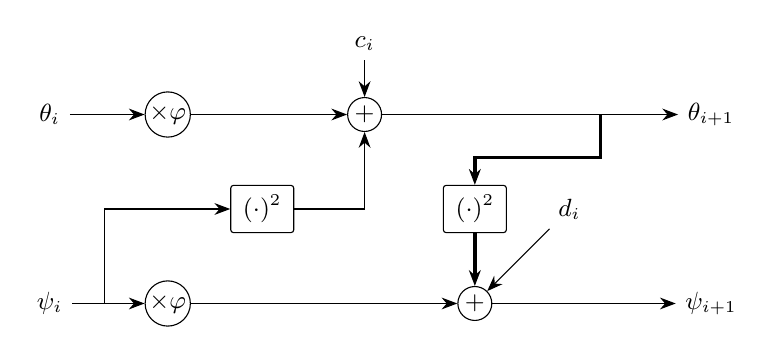
\begin{tikzpicture}[>={Stealth[length=2mm]}, font=\small,
  sq/.style={draw, rounded corners=1pt, minimum width=8mm, minimum height=6mm},
  add/.style={draw, circle, inner sep=1pt},
  mul/.style={draw, circle, inner sep=0.5pt}]
  % top rail (theta)
  \node (thin) at (0, 2.4) {$\theta_i$};
  \node[mul] (m1) at (1.5, 2.4) {$\times\varphi$};
  \node[add] (a1) at (4.0, 2.4) {$+$};
  \node (thout) at (8.4, 2.4) {$\theta_{i+1}$};
  % bottom rail (psi)
  \node (psin) at (0, 0) {$\psi_i$};
  \node[mul] (m2) at (1.5, 0) {$\times\varphi$};
  \node[add] (a2) at (5.4, 0) {$+$};
  \node (psout) at (8.4, 0) {$\psi_{i+1}$};
  % squarings
  \node[sq] (s1) at (2.7, 1.2) {$(\cdot)^2$};
  \node[sq] (s2) at (5.4, 1.2) {$(\cdot)^2$};
  % constants
  \node (ci) at (4.0, 3.3) {$c_i$};
  \node (di) at (6.6, 1.2) {$d_i$};
  % wires, top rail
  \draw[->] (thin) -- (m1);
  \draw[->] (m1) -- (a1);
  \draw[->] (a1) -- (thout);
  \draw[->] (ci) -- (a1);
  % psi squaring into top adder
  \draw[->] (0.7, 0) |- (s1.west);
  \draw[->] (s1.east) -| (a1.south);
  % wires, bottom rail
  \draw[->] (psin) -- (m2);
  \draw[->] (m2) -- (a2);
  \draw[->] (a2) -- (psout);
  \draw[->] (di) -- (a2);
  % coupling: tap AFTER the top adder
  \draw[->, very thick] (7.0, 2.4) |- (6.3, 1.85) -| (s2.north);
  \draw[->, very thick] (s2.south) -- (a2.north);
\end{tikzpicture}
\caption{Dataflow of one Mambo round
(Definition~\ref{def:mambo}). Each round costs exactly two nonlinear
constraints (the two squarings). The thick wire is the sequential
coupling: the second squaring consumes the \emph{updated} value
$\theta_{i+1}$, tapped after the first adder, not the input
$\theta_i$. The width-$t$ generalization
(Section~\ref{sec:inst:wider}) chains $t$ such squarings, each
feeding the next update in the same way.}
\label{fig:round}
\end{figure}

\paragraph{State width and the $t$-branch family.}
The definition above is the standard state-width-$2$ instance
($t = 2$) of a triangular-coupling family indexed by the state
width~$t \ge 2$. The generalization $M_{\varphi,i}\colon \Fp^{t} \to
\Fp^{t}$, in which $t$ sequential squarings each feed into the next,
is specified in Section~\ref{sec:inst:wider}. Every member of the
family preserves ALFOM~$\eta = 1.0$
(Proposition~\ref{prop:wider_alfom}). State width is an
instantiation parameter: selected jointly with the base field~$\Fp$
and the number of rounds~$n$ to meet a target security level
(Section~\ref{sec:security:parameters},
Table~\ref{tab:field-applicability}).


\subsection{R1CS Representation}\label{sec:map:r1cs}

Each application of $M_{\varphi,i}$ requires exactly two nonlinear constraints:
\begin{enumerate}[nosep]
  \item $\psi_i \cdot \psi_i = u_i$ (computes $u_i = \psi_i^2$), then
        $\theta_{i+1} = \varphi\cdot\theta_i + u_i + c_i$ is linear.
  \item $\theta_{i+1} \cdot \theta_{i+1} = v_i$ (computes
        $v_i = \theta_{i+1}^2$), then
        $\psi_{i+1} = \varphi\cdot\psi_i + v_i + d_i$ is linear.
\end{enumerate}
(The auxiliary witness symbols $u_i, v_i$ are chosen to avoid
collision with the state width~$t$.)
The round constants $c_i$ and $d_i$ enter only the linear constraints and
therefore do not contribute any additional nonlinear constraints.

\begin{proposition}[R1CS cost]\label{prop:cost}
The $n$-fold Mambo permutation $P_{\varphi,n}$ has R1CS cost $C = 2n$
nonlinear constraints.
\end{proposition}

\paragraph{MPC online cost.}
In the standard collaborative-SNARK / secret-shared-witness setting,
where each non-linear gate over a secret-shared field element costs one
online multiplication round and linear operations are local, the
per-permutation online MPC cost of $P_{\varphi,n}$ is exactly~$2n$
multiplication rounds ($164$ online multiplications at the
recommended $n = 82$).


\subsection{Design Rationale}\label{sec:map:rationale}

Three design choices are critical:

\paragraph{Coupled quadratics.}
A single iterated squaring $\theta_{i+1} = \theta_i^2 + c$ achieves degree
$2^n$ at cost~$n$, giving $\eta = 1.0$. However, this univariate map admits
efficient algebraic attacks. Coupling two variables forces each squaring to
amplify the degree of both components.

\paragraph{Sequential dependency.}
In a parallel coupling (using the old~$\theta$), the degree growth is
$d(n) = 2^n$, yielding $\eta = 0.5$. The sequential coupling---$\psi'$
depending on $\theta'$---doubles the effective degree per step from $2^n$ to
$4^n$ at no additional constraint cost, pushing $\eta$ from $0.5$ to~$1.0$.

\paragraph{Field independence.}
The map uses only field multiplication, field addition, the
constant~$\varphi$, and per-round constants $(c_i, d_i)$. No S-boxes, no
MDS matrices. The same definition works on any prime field with
$p \ge 2^{31}$.


\subsection{Round Constants}\label{sec:map:constants}

The Mambo permutation uses distinct round constants $(c_i, d_i) \in \Fp^2$
for each round $i \in \{0, \ldots, n-1\}$. These constants serve three
purposes:
\begin{enumerate}[nosep]
  \item \textbf{Fixed-point elimination.} Without round constants, $M_\varphi(0,0) = (0,0)$: the origin is a fixed point. Round constants ensure that the all-zero state is mapped to a nonzero output at every round.
  \item \textbf{Invariant subspace destruction.} Without constants, certain diagonal inputs $(\alpha,\alpha)$ map to diagonal outputs $(\beta,\beta)$, preserving a one-dimensional subspace. Distinct per-round constants break this symmetry.
  \item \textbf{Slide attack prevention.} Round constants destroy the shift invariance that otherwise permits slide attacks (Section~\ref{sec:security:slide}).
\end{enumerate}

\paragraph{Derivation.}
The $2n$ constants are derived deterministically from SHA-256 in
counter mode with the seed string \texttt{"Mambo\_round\_constants"}.
Specifically, for $j = 0, 1, \ldots, 2n-1$:
\[
  h_j = \mathrm{SHA\text{-}256}\bigl(\texttt{"Mambo\_round\_constants"} \,\|\, \mathrm{BE}_{32}(j)\bigr)\,,
\]
where $\mathrm{BE}_{32}(j)$ is the 32-bit big-endian encoding of~$j$.
Each $h_j$ is interpreted as a 256-bit unsigned integer and reduced
modulo~$p$; if the result is zero it is replaced with~$1$.
The round constants are then
$c_i = h_i \bmod p$ for $i \in \{0, \ldots, n-1\}$ and
$d_i = h_{n+i} \bmod p$ for $i \in \{0, \ldots, n-1\}$.

\paragraph{Impact on algebraic degree.}
The round constants are degree-0 terms in $\Fp[\theta_0, \psi_0]$ and
therefore do not affect the leading monomial at any step. The degree
recurrence (Lemma~\ref{lem:recurrence}) and the ALFOM of~1.0
(Corollary~\ref{cor:alfom}) are preserved exactly.

\paragraph{Impact on R1CS cost.}
In the R1CS representation, round constants enter only the linear
constraints (additions to~$\theta_{i+1}$ and~$\psi_{i+1}$). Adding a
constant is a free linear combination in R1CS: the nonlinear constraint
count remains $C = 2n$.

\paragraph{Domain separation across state widths.}
Wider-state variants ($t \geq 3$) use a distinct seed string so that
round constants for the narrow ($t=2$) primitive cannot be re-used as
constants for a wider primitive (or vice versa). The $t=2$ seed is
\texttt{"Mambo\_round\_constants"} as above; the $t=4$ seed is
\texttt{"Mambo\_t4\_round\_constants"}. Higher widths follow the same
\texttt{Mambo\_t$\langle t\rangle$\_round\_constants} pattern. This
enforces cross-variant domain separation at the primitive level so that
a commitment produced under one state width cannot collide with a
commitment produced under a different width even at identical inputs.
Reference implementations verify consistency against these seeds at
build time.


\subsection{Relation to Feistel Networks and Existing Quadratic
Structures}\label{sec:map:feistel}

\paragraph{The Feistel reading.}
One Mambo round (Definition~\ref{def:mambo}) can be read as two
consecutive unbalanced Feistel steps with round function $f(x) = x^2$
and branch multiplier~$\varphi$: the first step updates $\theta$ in
place as $\theta \mapsto \varphi\theta + f(\psi) + c_i$, the second
updates $\psi$ in place as $\psi \mapsto \varphi\psi + f(\theta') +
d_i$. Up to the $\varphi$-scaling of the recycled branch and the
absence of a branch swap (the update is written in place; the swap is
absorbed into the alternation of the two steps), this is the oldest
skeleton in symmetric cryptography, instantiated with the lowest-degree
nonlinearity a prime field offers. We state this plainly because the
skeleton is also current: the algebraic rounds of
Skyscraper~\cite{Skyscraper} are exactly such steps, $(x_L, x_R)
\mapsto (x_R + x_L^2/\sigma + \gamma_i,\; x_L)$ with $\sigma$ a
Montgomery constant, and Feistel--MiMC~\cite{MiMC,Bariant_CICO} is the
same skeleton with $f(x) = x^3$. Mambo's contribution is not the
skeleton; it is the exact algebraic characterization that this
particular instantiation of the skeleton admits, which we make precise
below.

\paragraph{Composition versus parallel application.}
The Feistel reading makes the role of the sequential coupling exact.
Because $\psi'$ consumes the \emph{updated} value $\theta'$ within the
same round, the $2n$ squarings of $P_{\varphi,n}$ form a single
composition chain: every squaring acts on a state component carrying
the maximal degree produced so far, and the degree doubles at every
nonlinear constraint, giving total degree $4^n$ at cost $2n$
(Theorem~\ref{thm:degree}). The structural alternative --- applying the
two quadratics in parallel to the \emph{old} state, $\theta' =
\varphi\theta + \psi^2 + c_i$, $\psi' = \varphi\psi + \theta^2 + d_i$
--- is a two-branch SPN rather than a Feistel network; its degree
growth is $2^n$ at the same cost, i.e.\ $\eta = 0.5$. Squaring is the
unique round function for which this composition extracts the full
R1CS bound: a power map $x^{\alpha}$ costs $\lceil \log_2 \alpha
\rceil$ constraints but multiplies the degree by~$\alpha$, with
equality of the two only at $\alpha = 2$. The $\varphi$-scaling of the
recycled branch keeps each step invertible without a swap
(Remark~\ref{rem:invert}), breaks the branch-interchange and slide
symmetries of an unscaled Feistel chain, and is the hypothesis
($\varphi \ge 2$) under which the no-cancellation argument of
Theorem~\ref{thm:degree} holds for every prime $p > 2$.

\paragraph{Delineation from existing quadratic and Feistel-type AO designs.}
MiMC~\cite{MiMC} iterates the univariate cube: each round costs two
constraints and multiplies the degree by~$3$, so $n$ rounds give degree
$3^n$ at cost $2n$, i.e.\ $\eta = \log_2 3 / 2 \approx 0.79$; the same
accounting applies to its Feistel variant. The open
Flystel~\cite{Anemoi} (Anemoi's butterfly) deliberately splits the two
directions: the verification relation is quadratic while one
evaluation direction involves a high-degree power map $x^{1/\alpha}$,
so the security argument rests on the degree asymmetry between
CCZ-equivalent representations rather than on proven degree growth of
the iterated map --- and the published algebraic attacks on Anemoi
target precisely the low-degree representation~\cite{Anemoi_attack,FreeLunch}.
Horst~\cite{Griffin}, Griffin's nonlinear mode, replaces Feistel's
additive combination $L + f(R)$ by the multiplicative $L \cdot G(R)$:
degrees of distinct branches \emph{add}, which is efficient but does
not double the maximal degree per constraint, and the resulting
systems proved vulnerable to dedicated
solvers~\cite{FreeLunch,Griffin_break}. Skyscraper~\cite{Skyscraper}
is the closest published relative at the level of the round step, but
the design intent is orthogonal: of its ten Feistel rounds only six
are squarings (used for cheap native nonlinearity), the remaining four
are lookup-based ``Bars'' rounds carrying the statistical security,
and no exact algebraic claims are made for the composition. Its
cryptanalytic record --- a practical rebound distinguisher on the full
permutation~\cite{Skyscraper_dist} and full-round attacks combining
cheap polynomial solving across the quadratic rounds with statistical
properties of the lookup rounds~\cite{Skyscraper_break}, answered by
the revised Skyscraper-v2~\cite{Skyscraper} --- illustrates that a
\emph{short} quadratic Feistel chain is algebraically cheap to
traverse. Mambo draws the opposite conclusion from the same skeleton:
it uses \emph{only} the quadratic Feistel step, iterates it $2n$ times
with $n$ sized so that the eliminant degree meets the security
target, and prices the entire attack surface by the proven growth of
the algebraic invariants rather than by interleaved non-algebraic
components.

\paragraph{Prior exact-degree results, and what
Theorem~\ref{thm:degree} adds.}
The degree growth of iterated low-degree maps has been studied most
intensively for MiMC. Eichlseder et
al.~\cite{MiMC_fulldegree} proved a nontrivial \emph{upper} bound on
the growth of the $\mathbb{F}_2$-algebraic degree of MiMC-like
iterates over binary fields, yielding a higher-order distinguisher on
full MiMC; Bouvier, Canteaut, and Perrin~\cite{MiMC_exactdegree}
subsequently determined the \emph{exact} algebraic degree of iterated
$x^3$ for large round ranges, exhibiting plateaus where the degree
does not grow at all for consecutive rounds; and Cid et
al.~\cite{Cid_linlayer} showed that the linear layer can degrade the
growth from exponential to linear in SP-networks. Three features
distinguish those results from Theorem~\ref{thm:degree}. First, they
concern the $\mathbb{F}_2$-algebraic degree over binary extension
fields --- the invariant relevant to higher-order differential
attacks there --- whereas over a prime field the relevant invariant is
the total degree of the iterated polynomials, which is the one Mambo
characterizes. Second, they are obtained a posteriori, by intricate
exponent tracing applied to a fixed published design, and are exact
only for specific maps and round ranges; the plateau phenomenon they
uncover shows that maximal growth cannot be assumed in general.
Third, none of them yields the ideal-theoretic data that algebraic
attack costs are actually priced in. For Mambo the situation is
inverted by construction: the sequential quadratic coupling forces the
degree recurrence to meet its upper branch with equality at every
step, for every $p > 2$ and every $\varphi \ge 2$, and the same
triangular structure makes the CICO ideal explicit enough that its
Gr\"obner basis, Hilbert series, regularity degree $d_{\mathrm{reg}} =
2n$, and eliminant degree are closed-form theorems
(Section~\ref{sec:security:groebner},
Appendix~\ref{app:dreg_proof}) rather than empirical estimates. The
Feistel lineage is thus a feature of the design: the skeleton is what
makes the construction fully analyzable, and the analysis ---
including the resulting attack costs --- is carried out in this paper
rather than left to future cryptanalysis.


%=============================================================================
\section{Degree Growth Analysis}\label{sec:degree}
%=============================================================================

This section contains the main algebraic result.

\subsection{Degree Recurrence}\label{sec:degree:recurrence}

Let $d_\theta(n)$ and $d_\psi(n)$ denote the total degree of $\theta_n$ and
$\psi_n$ as polynomials in $\Fp[\theta_0, \psi_0]$.

\begin{lemma}[Degree recurrence]\label{lem:recurrence}
\begin{align}
  d_\theta(n) &= \max\bigl(d_\theta(n-1),\; 2\,d_\psi(n-1)\bigr)\,,
  \label{eq:rec_theta} \\
  d_\psi(n)   &= 2\,d_\theta(n)\,.  \label{eq:rec_psi}
\end{align}
\end{lemma}

\begin{proof}
From~\eqref{eq:theta}: $\theta_n = \varphi\cdot\theta_{n-1} + \psi_{n-1}^2 + c_{n-1}$.
The term $\varphi\cdot\theta_{n-1}$ has degree $d_\theta(n-1)$,
$\psi_{n-1}^2$ has degree $2\,d_\psi(n-1)$, and the round constant $c_{n-1}$
has degree~0. Their sum has degree
$\max(d_\theta(n-1), 2\,d_\psi(n-1))$, provided the leading-degree terms do
not cancel (see Theorem~\ref{thm:degree}).

From~\eqref{eq:psi}: $\psi_n = \varphi\cdot\psi_{n-1} + \theta_n^2 + d_{n-1}$.
Since $2\,d_\theta(n) > d_\psi(n-1)$ for $n \ge 1$, the squared term
dominates and the degree-0 constant $d_{n-1}$ is absorbed:
$d_\psi(n) = 2\,d_\theta(n)$.
\end{proof}


\subsection{Main Result: Exact Degree Growth}\label{sec:degree:main}

\begin{theorem}[Degree growth]\label{thm:degree}
For all $n \ge 1$,
\[
  d_\psi(n) = 4^n\,,\qquad d_\theta(n) = \tfrac{4^n}{2} = 2\cdot 4^{n-1}\,.
\]
Moreover, the leading-degree homogeneous components of $\theta_n$ and
$\psi_n$ are nonzero; no cancellation occurs at the top degree.
\end{theorem}

\begin{proof}
We proceed by strong induction on~$n$.

\emph{Base case ($n=1$).} Starting from $(\theta_0, \psi_0)$, both of
degree~1:
\begin{align*}
  \theta_1 &= \varphi\cdot\theta_0 + \psi_0^2 + c_0\,,\\
  \psi_1   &= \varphi\cdot\psi_0 + (\varphi\cdot\theta_0 + \psi_0^2 + c_0)^2 + d_0\,.
\end{align*}
Expanding, the leading term of~$\psi_1$ is $\psi_0^4$; the constants
$c_0, d_0$ contribute only degree-0 and lower-degree cross terms.
We have $d_\theta(1) = 2$ and $d_\psi(1) = 4 = 4^1$.

\emph{Inductive step.} Assume for all $k \le n-1$: $d_\psi(k) = 4^k$ and
$d_\theta(k) = 4^k/2$. By Lemma~\ref{lem:recurrence}:
\begin{align*}
  d_\theta(n) &= \max\!\left(\tfrac{4^{n-1}}{2},\; 2\cdot 4^{n-1}\right)
               = 2\cdot 4^{n-1} = \tfrac{4^n}{2}\,,\\
  d_\psi(n)   &= 2\,d_\theta(n) = 4^n\,.
\end{align*}

\emph{Non-cancellation argument.} Consider
$\theta_n = \varphi\cdot\theta_{n-1} + \psi_{n-1}^2 + c_{n-1}$. The degree of
$\varphi\cdot\theta_{n-1}$ is $4^{n-1}/2$, $\psi_{n-1}^2$ has degree
$2\cdot 4^{n-1}$, and $c_{n-1}$ has degree~0.
Since $2\cdot 4^{n-1} > 4^{n-1}/2$, the leading terms
come \emph{exclusively} from $\psi_{n-1}^2$---the square of the leading
homogeneous component of~$\psi_{n-1}$, which is nonzero by induction (the
square of a nonzero polynomial over a field of characteristic $p > 2$ is
nonzero). The constant $c_{n-1}$ cannot affect the leading monomial.

For $\psi_n = \varphi\cdot\psi_{n-1} + \theta_n^2 + d_{n-1}$: the degree of
$\varphi\cdot\psi_{n-1}$ is $4^{n-1}$, while $\theta_n^2$ has degree~$4^n$
and $d_{n-1}$ has degree~0.
Since $4^n > 4^{n-1}$, the leading terms come exclusively from~$\theta_n^2$.

At no step do leading-degree terms from different sources combine, so no
cancellation can occur.
\end{proof}

The non-cancellation argument is stronger than typical for iterated
polynomial maps: the strict degree separation between the linear term
and the quadratic term ensures single-source dominance at every
step---a structural consequence of the sequential coupling.


\subsection{Corollary: ALFOM = 1.0}\label{sec:degree:alfom}

\begin{corollary}[ALFOM = 1.0]\label{cor:alfom}
The Mambo permutation $P_{\varphi,n}$ has
\[
  \eta = \frac{\log_2(d_\psi(n))}{C}
       = \frac{\log_2(4^n)}{2n}
       = \frac{2n}{2n} = 1.0\,.
\]
This holds for all $n \ge 1$, independently of the field~$\Fp$ and the
parameter~$\varphi$.
\end{corollary}

The ALFOM of~1.0 is an unconditional algebraic fact: it does not
depend on any security assumption or heuristic, and round constants,
being degree-0 elements of $\Fp[\theta_0, \psi_0]$, cannot alter the
leading monomial or the degree count at any step. The metric should
also be deflated correctly: $\eta$ measures algebraic degree per
nonlinear constraint, not attack cost, and the trivial iterated
squaring chain $x \mapsto x^2 + c$ attains $\eta = 1.0$ while being
cryptographically worthless (univariate and invertible by repeated
square-root extraction; Section~\ref{sec:map:rationale}). Hence
$\eta = 1.0$ is necessary for constraint-optimal degree growth but
not sufficient for security, and the security content of this paper
lives in the exact characterization and the analysis of
Section~\ref{sec:security}, not in the metric.


\subsection{Comparison with Clotho}\label{sec:degree:clotho}

Clotho ($\beta = 2$), introduced in~\cite{ALFOMs}, also achieves
$\eta = 1.0$. The two constructions reach the bound by different mechanisms:
Clotho uses a power map $x \mapsto x^\beta$ with a carefully chosen linear
layer; Mambo uses two coupled quadratic equations with sequential
dependency. Whether all $\eta = 1.0$ R1CS constructions share a common
algebraic characterization is an open question.


\subsection{Non-Telescoping Property}\label{sec:degree:nontelescoping}

Throughout this subsection fix an odd prime~$p$, a parameter
$\varphi \in \Fp$, and round constants
$c_0, d_0, \ldots, c_{n-1}, d_{n-1} \in \Fp$, and write
$\Theta_i, \Psi_i \in \Fp[\theta_0, \psi_0]$ for the round-$i$ iterates
($\Theta_0 = \theta_0$, $\Psi_0 = \psi_0$). The sponge-CICO
specialisation sets $\psi_0 = 0$ and fixes the rate output
$\theta_n = \tau$; we write $F_i(a) := \Theta_i(a, 0)$,
$G_i(a) := \Psi_i(a, 0)$, and $f_n(a) := F_n(a) - \tau$.

For integer weights $w_x, w_y \ge 1$ let $\deg_w$ denote the weighted
degree on $\Fp[x, y]$ with $\deg_w x = w_x$, $\deg_w y = w_y$, and call
the sum of the terms of maximal weighted degree the \emph{top
$w$-component}. Top $w$-components are multiplicative over a field. Two
lemmas isolate the structure that prevents telescoping.

\begin{lemma}[Single-monomial dominance under substitution]\label{lem:dominance}
Let $K$ be a field and let $P \in K[x, y]$ have, for weights
$(w_x, w_y)$, top $w$-component equal to a single monomial
$\lambda y^{J}$ with $\lambda \ne 0$ and $J \ge 1$. Let $F, G \in K[a]$
satisfy $\deg F \le d\,w_x$ and $\deg G = d\,w_y$ exactly, for some
integer $d \ge 1$. Then
\[
  \deg_a P(F, G) \;=\; d\,J\,w_y,
  \qquad
  \operatorname{lc}\bigl(P(F, G)\bigr)
   \;=\; \lambda\,\operatorname{lc}(G)^{J}.
\]
The same statement holds with the roles of $x$ and $y$ exchanged.
\end{lemma}

\begin{proof}
A monomial $x^i y^j$ of $P$ contributes degree at most
$i \deg F + j \deg G \le d\,(i w_x + j w_y)$ to $P(F, G)$. Every
monomial of $P$ other than $y^{J}$ has weighted degree at most
$J w_y - 1$ (a monomial of weighted degree $J w_y$ would belong to the
top $w$-component), hence contributes degree at most
$d(J w_y - 1) < d J w_y$. The monomial $\lambda y^{J}$ contributes
$\lambda \operatorname{lc}(G)^{J} a^{d J w_y}$ plus lower-order terms,
and $\lambda \operatorname{lc}(G)^{J} \ne 0$ over a field.
\end{proof}

\begin{lemma}[Weighted structure of partial compositions]\label{lem:partial_weights}
Fix $r \ge 1$ and constants
$c'_0, d'_0, \ldots, c'_{r-1}, d'_{r-1} \in \Fp$, and let
$\Theta'_k, \Psi'_k \in \Fp[x, y]$ be the $k$-round iterates from a
free state $(x, y)$ under these constants. For each of the weightings
$(w_x, w_y) \in \{(1, 1),\, (1, 2)\}$ and every $1 \le k \le r$, the
top $w$-components of $\Theta'_k$ and $\Psi'_k$ are the single
monomials
\[
  \operatorname{top}_w \Theta'_k \;=\; y^{2 \cdot 4^{k-1}},
  \qquad
  \operatorname{top}_w \Psi'_k \;=\; y^{4^{k}},
\]
each with coefficient~$1$. The analogous statement holds for a chain
entered at the $\psi$-update (first map
$(u, v) \mapsto \varphi v + u^2 + d'$, then full rounds) with weights
$(w_u, w_v) = (2, 1)$: the dominant monomials are the corresponding
pure powers of~$u$, with coefficient~$1$. All statements hold in every
characteristic, for every $\varphi$, and for arbitrary constants.
\end{lemma}

\begin{proof}
Induction on~$k$; we write the case $(w_x, w_y) = (1, 2)$, the other
two being the same computation. For $k = 1$:
$\Theta'_1 = \varphi x + y^2 + c'_0$ has summands of $w$-degree
$1, 4, 0$, so $\operatorname{top}_w \Theta'_1 = y^2$;
$\Psi'_1 = \varphi y + (\Theta'_1)^2 + d'_0$, and
$\operatorname{top}_w (\Theta'_1)^2 = (y^2)^2 = y^4$ has $w$-degree
$8 > 2$, so $\operatorname{top}_w \Psi'_1 = y^4$. For the step:
in $\Theta'_{k+1} = \varphi \Theta'_k + (\Psi'_k)^2 + c'_k$ the square
has top $w$-component $(y^{4^k})^2 = y^{2 \cdot 4^k}$ of $w$-degree
$4^{k+1}$, strictly exceeding $\deg_w \Theta'_k = 4^k$; in
$\Psi'_{k+1} = \varphi \Psi'_k + (\Theta'_{k+1})^2 + d'_k$ the square
has top $w$-component $y^{4^{k+1}}$ of $w$-degree
$2 \cdot 4^{k+1} > 2 \cdot 4^k$. At every step the top $w$-component
comes from a single source and is the square of a single monomial with
coefficient~$1$.
\end{proof}

\begin{proposition}[Non-telescoping]\label{prop:nontelescoping}
Let
$S = \Fp[\theta_0, \psi_0, \theta_1, \psi_1, \ldots, \theta_n, \psi_n]$
and let $J_n \subset S$ be the ideal generated by the $2n$ round
relations $\theta_i - \varphi \theta_{i-1} - \psi_{i-1}^2 - c_{i-1}$
and $\psi_i - \varphi \psi_{i-1} - \theta_i^2 - d_{i-1}$,
$1 \le i \le n$.
\begin{enumerate}[nosep, label=(\roman*)]
\item \textbf{Free-input elimination floor.}
$\bigl(J_n + (\psi_n - \tau)\bigr) \cap \Fp[\theta_0, \psi_0]
 = \bigl(\Psi_n(\theta_0, \psi_0) - \tau\bigr)$ is principal,
generated by a polynomial of total degree exactly~$4^{n}$ whose
leading form is the single monomial $\psi_0^{4^{n}}$. Hence every
nonzero polynomial in $(\theta_0, \psi_0)$ alone lying in the ideal of
the round system has total degree at least~$4^{n}$: the intermediate
states cannot be algebraically eliminated below degree~$4^n$. This
holds over every field, for every~$\varphi$, and for every choice of
round constants.
\item \textbf{CICO elimination floor.} Assume $\varphi \ne 0$
in~$\Fp$. Then
$\bigl(J_n + (\psi_0,\, \theta_n - \tau)\bigr) \cap \Fp[\theta_0]
 = (f_n)$ with $\deg f_n = 4^{n-1} = D_I$ and
$\operatorname{lc}(f_n) = \varphi^{4^{n-1}} \ne 0$. Hence every
nonzero univariate consequence of the sponge-CICO system in the rate
input---the output of any elimination procedure whatsoever, including
iterated resultants and Gr\"obner bases, since both produce elements
of the ideal---has degree at least~$D_I$.
\item \textbf{Variety floor.} For every fixed round-constant tuple
(with $\varphi \ne 0$), $f_n$ is squarefree for all but at most
$D_I - 1$ targets $\tau \in \Fp$. For such~$\tau$ the CICO system has
exactly $D_I$ distinct solutions over~$\overline{\Fp}$, and
consequently \emph{any} polynomial reformulation of the system---in
particular any meet-in-the-middle organisation, one- or two-sided, at
any cut point---admits no nonzero $g \in \overline{\Fp}[\theta_0]$ of
degree $< D_I$ whose root set contains all solutions.
\item \textbf{Split exactness.} For every cut of the $2n$-equation
chain---after the $\psi$-update of round~$m$ (middle state
$(\theta_m, \psi_m)$, $1 \le m \le n-1$) or after the $\theta$-update
of round~$m$ (middle state $(\theta_m, \psi_{m-1})$,
$2 \le m \le n-1$)---the meeting polynomial obtained by substituting
the forward half-iterates into the backward half-constraint equals
$f_n$ identically: its degree is exactly~$4^{n-1}$ with leading
coefficient~$\varphi^{4^{n-1}}$, independent of the cut. No choice of
meeting point lowers the degree at which the two halves meet.
\end{enumerate}
\end{proposition}

\begin{proof}
\emph{(i)} Order the variables
$\theta_0 \prec \psi_0 \prec \theta_1 \prec \psi_1 \prec \cdots$; each
round relation rewrites one variable as a polynomial in strictly
earlier ones. Let $\epsilon : S \to \Fp[\theta_0, \psi_0]$ be the
evaluation homomorphism fixing $\theta_0, \psi_0$ and sending
$\theta_i \mapsto \Theta_i$, $\psi_i \mapsto \Psi_i$. By induction
along the order, $\theta_i \equiv \Theta_i$ and
$\psi_i \equiv \Psi_i \pmod{J_n}$, hence
$g \equiv \epsilon(g) \pmod{J_n}$ for every $g \in S$ (substituting
congruent elements into a polynomial preserves congruence). Write
$I = J_n + (\psi_n - \tau)$. Since $\epsilon$ kills every round
relation and $\epsilon(\psi_n - \tau) = \Psi_n - \tau$, and $\epsilon$
is a ring homomorphism into $\Fp[\theta_0, \psi_0]$, we get
$\epsilon(I) \subseteq (\Psi_n - \tau)$. If
$g \in I \cap \Fp[\theta_0, \psi_0]$ then
$g = \epsilon(g) \in (\Psi_n - \tau)$; conversely
$\Psi_n - \tau = (\psi_n - \tau) - (\psi_n - \Psi_n) \in I$. The
degree~$4^n$ and the monic leading form $\psi_0^{4^n}$ are
Theorem~\ref{thm:degree} together with the $(1,1)$-weighted case of
Lemma~\ref{lem:partial_weights} at $k = n$. Degrees add over a domain,
so every nonzero multiple of $\Psi_n - \tau$ in
$\Fp[\theta_0, \psi_0]$ has total degree at least~$4^n$.

\emph{(ii)} Identical, with the evaluation
$\epsilon^{\circ} : S \to \Fp[\theta_0]$ sending $\psi_0 \mapsto 0$,
$\theta_i \mapsto F_i$, $\psi_i \mapsto G_i$; the elimination ideal is
$(f_n)$. Degree and leading coefficient follow from the specialised
recursion $F_1 = \varphi \theta_0 + c_0$, $G_1 = F_1^2 + d_0$, and,
for $i \ge 1$, $F_{i+1} = \varphi F_i + G_i^2 + c_i$,
$G_{i+1} = \varphi G_i + F_{i+1}^2 + d_i$: since
$\deg G_i^2 = 4^{i} > 4^{i-1} = \deg F_i$ and
$\deg F_{i+1}^2 = 2 \cdot 4^{i} > 2 \cdot 4^{i-1} = \deg G_i$, the top
term comes from a single source at every step, giving by induction
\[
  \deg F_i = 4^{i-1}, \quad
  \operatorname{lc} F_i = \varphi^{4^{i-1}}, \quad
  \deg G_i = 2 \cdot 4^{i-1}, \quad
  \operatorname{lc} G_i = \varphi^{2 \cdot 4^{i-1}},
\]
all nonzero because $\varphi \ne 0$. (If $p \mid \varphi$ the system
degenerates---$F_1$ is constant---so the hypothesis is sharp.)

\emph{(iii)} Write $f_n = h - \tau$ with $h := F_n$. Since $p$ is odd
and $D_I = 2^{2(n-1)}$, we have $p \nmid D_I$; by the discriminant
formula for $h(x) - c$ already used in the proof of
Theorem~\ref{thm:generic_sqfree}
(Gelfand--Kapranov--Zelevinsky~\cite{GKZ1994}, Ch.~12),
$\operatorname{disc}(f_n)$ is a polynomial in~$\tau$ of degree exactly
$D_I - 1$ with leading coefficient
$\pm D_I^{D_I} \varphi^{D_I(D_I - 1)} \ne 0$, so it vanishes for at
most $D_I - 1$ values of~$\tau$. For all other~$\tau$, $f_n$ has $D_I$
distinct roots in~$\overline{\Fp}$, each a CICO solution, and any~$g$
vanishing on all of them is a multiple of~$f_n$ up to a scalar, hence
$\deg g \ge D_I$. This argument references only the solution set, not
the algebraic form in which an attacker carries the system; it
therefore applies to every sound reorganisation of the equations,
including meet-in-the-middle systems built from forward iterates,
from inverse-round iterates entering at the output side, or both.

\emph{(iv)} Cut after the $\psi$-update of round~$m$, middle state
$(x, y) = (\theta_m, \psi_m)$. The backward half-constraint is
$P_{n-m}(x, y) := \Theta'_{n-m}(x, y) - \tau$, where $\Theta'_{n-m}$
is the $(n-m)$-round iterate of Lemma~\ref{lem:partial_weights} under
the constants of rounds $m+1, \ldots, n$; the additive constant
$-\tau$ does not change the top $w$-component, which is
$y^{2 \cdot 4^{n-m-1}}$ with coefficient~$1$ for the weights
$(1, 2)$. The forward half-iterates satisfy
$\deg F_m = 4^{m-1} = d \cdot 1$ and
$\deg G_m = 2 \cdot 4^{m-1} = d \cdot 2$ exactly, with $d = 4^{m-1}$
and $\operatorname{lc}(G_m) = \varphi^{2 \cdot 4^{m-1}} \ne 0$, by the
recursion in~(ii). Lemma~\ref{lem:dominance} gives
\[
  \deg_a P_{n-m}(F_m, G_m)
   = 4^{m-1} \cdot 2 \cdot 4^{n-m-1} \cdot 2 = 4^{n-1},
  \qquad
  \operatorname{lc}
   = \bigl(\varphi^{2 \cdot 4^{m-1}}\bigr)^{2 \cdot 4^{n-m-1}}
   = \varphi^{4^{n-1}},
\]
and $P_{n-m}(F_m, G_m) = f_n$ identically by associativity of
composition. For a cut after the $\theta$-update of round~$m$
($m \ge 2$), the middle state is $(u, v) = (\theta_m, \psi_{m-1})$
with $\deg F_m = 4^{m-1} = d' \cdot 2$ and
$\deg G_{m-1} = 4^{m-1}/2 = d' \cdot 1$, $d' = 4^{m-1}/2$; the
backward chain is entered at the $\psi$-update, and by the last part
of Lemma~\ref{lem:partial_weights} its top $w$-component for the
weights $(2, 1)$ is the single monomial $u^{4^{n-m}}$ with
coefficient~$1$. Lemma~\ref{lem:dominance}, with the roles of the
variables exchanged, gives degree
$d' \cdot 4^{n-m} \cdot 2 = 4^{n-1}$ and leading coefficient
$\bigl(\varphi^{4^{m-1}}\bigr)^{4^{n-m}} = \varphi^{4^{n-1}}$, and the
meeting polynomial is again $f_n$ identically.
\end{proof}

\begin{corollary}[Middle-state eliminant]\label{cor:middle_eliminant}
Assume $\varphi \ne 0$, fix a cut after round~$m$, and let
$A := \Fp[a]/(f_n)$ and $\beta := F_m(a) \bmod f_n \in A$, the image
of the middle coordinate~$\theta_m$. The univariate consequences of
the CICO system in~$\theta_m$ form the principal ideal generated by
the minimal polynomial~$\mu_\beta$ of~$\beta$, and the canonical
eliminant computable from the half-systems,
\[
  E_m(x)
   \;=\; \det\bigl(x \cdot \mathrm{Id} - M_\beta\bigr)
   \;=\; \operatorname{lc}(f_n)^{-4^{m-1}}\,
         \operatorname{Res}_a\bigl(f_n(a),\, x - F_m(a)\bigr),
\]
with $M_\beta$ the multiplication-by-$\beta$ matrix on~$A$, is monic
of degree exactly~$D_I$. If moreover $f_n$ is squarefree and $F_m$
separates the roots of~$f_n$ in~$\overline{\Fp}$, then
$\mu_\beta = E_m$ has degree~$D_I$: every nonzero univariate
consequence in the middle coordinate also has degree at
least~$D_I$, so meeting in the middle does not reduce the effective
univariate degree on the middle coordinate either. The separation
condition is Zariski-open in $(c_0, \ldots, d_{n-1}, \tau)$: the
coefficients of $E_m$ are polynomials in~$\tau$ of degree at
most~$4^{m-1}$, so once $E_m$ is squarefree at a single
target~$\tau^{*}$, separation can fail for at most
$(2 D_I - 1)\, 4^{m-1}$ targets~$\tau$. For the production constants
of Section~\ref{sec:map:constants} such certificates were computed
for all splits $1 \le m \le n-1$ at $n \in \{2, \ldots, 6\}$ over
both production fields (Section~\ref{sec:degree:verification}).
\end{corollary}

\begin{proof}
By the evaluation argument of
Proposition~\ref{prop:nontelescoping}(ii), a polynomial
$q(\theta_m)$ lies in the CICO ideal iff $q(F_m) \in (f_n)$, i.e.\
iff $q(\beta) = 0$ in~$A$, i.e.\ iff $\mu_\beta \mid q$. The algebra
$A$ is free of rank~$D_I$ with basis $1, a, \ldots, a^{D_I - 1}$, so
$E_m$ is monic of degree~$D_I$; the resultant expression is the
standard product formula
$\operatorname{Res}_a(f_n, x - F_m)
 = \operatorname{lc}(f_n)^{4^{m-1}} \prod_i \bigl(x - F_m(a_i)\bigr)$
over the roots $a_i$ of~$f_n$ with multiplicity. If $f_n$ is
squarefree, $A \otimes \overline{\Fp} \cong \overline{\Fp}^{\,D_I}$
with $\beta \mapsto (F_m(a_i))_i$, so
$\mu_\beta = \prod_{v \in \{F_m(a_i)\}} (x - v)$ and
$\deg \mu_\beta = D_I$ iff the values $F_m(a_i)$ are pairwise
distinct, iff $E_m$ is squarefree. For the $\tau$-degree bound:
in $\operatorname{Res}_a(F_n(a) - \tau,\, x - F_m(a))$ the Sylvester
matrix contains $\tau$ only in the $4^{m-1}$ rows carrying the
coefficients of $f_n$, each linearly, so
$\deg_\tau E_m \le 4^{m-1}$; hence
$\operatorname{disc}_x(E_m) \in \Fp[\tau]$ has degree at most
$(2 D_I - 1)\, 4^{m-1}$, and a single $\tau^{*}$ with
$\operatorname{disc}_x(E_m)(\tau^{*}) \ne 0$ shows it is not
identically zero.
\end{proof}

\begin{remark}[Scope]\label{rem:nontelescoping_scope}
Proposition~\ref{prop:nontelescoping} is a statement about algebraic
degrees, not running time: it proves that no elimination strategy---in
particular no meet-in-the-middle organisation of the rounds---produces
a univariate constraint of degree below~$D_I$, so the cost model of
Section~\ref{sec:security:costmodel} prices every such strategy at the
same $\widetilde{O}(\min(D_I, p))$ univariate figure. It does not (and
cannot) rule out faster algorithms for the root-finding step itself;
that is the content of Conjecture~\ref{conj:cico}. The separation
hypothesis of Corollary~\ref{cor:middle_eliminant}---certified at the
production constants for all splits at $n \in \{2, \ldots, 6\}$ over
both production fields---gates only the middle-coordinate
meet-in-the-middle variant; the unconditional rate-input floors
(i)--(iv) do not depend on it.
\end{remark}


\subsection{Symbolic Verification}\label{sec:degree:verification}

We verified the degree formulas symbolically using SageMath for
$n = 1, \ldots, 8$ by computing the explicit polynomials over
$\mathbb{Q}(\varphi)$. The non-telescoping battery of
Proposition~\ref{prop:nontelescoping} and
Corollary~\ref{cor:middle_eliminant}---per-round degrees and leading
coefficients, monic free-input leading forms, split exactness at every
cut, and the full-degree middle-state minimal-polynomial
certificates---is reproduced by \texttt{analysis/nontelescoping\_verify.sage}
at the production constants for $n = 2, \ldots, 6$ over both production
fields.

\begin{table}[h]
\centering
\caption{Symbolic verification of degree growth.}
\label{tab:degree}
\begin{tabular}{@{}rrrrr@{}}
\toprule
$n$ & $d_\theta(n)$ & $d_\psi(n)$ & $\log_2 d_\psi$ & Status \\
\midrule
1 & 2 & 4 & 2 & Verified \\
2 & 8 & 16 & 4 & Verified \\
3 & 32 & 64 & 6 & Verified \\
4 & 128 & 256 & 8 & Verified \\
5 & 512 & 1\,024 & 10 & Verified \\
6 & 2\,048 & 4\,096 & 12 & Verified \\
7 & 8\,192 & 16\,384 & 14 & Verified \\
8 & 32\,768 & 65\,536 & 16 & Verified \\
\bottomrule
\end{tabular}
\end{table}


%=============================================================================
\section{Security Analysis}\label{sec:security}
%=============================================================================

\subsection{Security Framework and Assumptions}\label{sec:security:framework}

The security of Mambo is organised in three layers, following the
standard architecture for fixed unkeyed permutations:
\begin{enumerate}[nosep]
  \item \textbf{Mode bounds, proven in the ideal-permutation model.}
        Replacing $P_{\varphi,n}$ by a uniformly random permutation,
        the sponge collision and indifferentiability bounds
        (Proposition~\ref{prop:sponge_sec},
        Corollary~\ref{thm:collision}, via BDPV08~\cite{BDPV08}) and
        the PRNG indistinguishability bound
        (Lemma~\ref{lem:hcp_from_prp}) hold unconditionally with the
        stated birthday terms.
  \item \textbf{One explicitly labeled design claim}
        (Design Claim~\ref{claim:structural}) asserting that the
        concrete permutation admits no structural distinguisher below
        the target cost. This calibrates when the ideal-permutation
        modeling of layer~1 is sound; it is the single assumption of
        the paper.
  \item \textbf{One falsifiable CICO-hardness conjecture}
        (Conjecture~\ref{conj:cico}), parameterized over $(t, n, p)$
        so that it covers every parameter set of
        Table~\ref{tab:tiers}, minimum and recommended rows alike. It is the
        sharpest concrete consequence of the design claim on the
        algebraic attack surface, and the statement we invite the
        community to attack. The remainder of this section collects
        the evidence for it.
\end{enumerate}

\begin{designclaim}[No structural distinguisher]\label{claim:structural}
For every parameter set $(t, n, \Fp, \varphi)$ of
Table~\ref{tab:tiers} (minimum or recommended row) at security
level~$\lambda$, no algorithm given
the full circuit description distinguishes the Mambo permutation
$P_{\varphi,n}$ on~$\Fp^t$ from a uniformly random permutation at cost
below~$2^{\lambda}$, beyond the generic and algebraic attacks
accounted for in this section.
\end{designclaim}

Design Claim~\ref{claim:structural} is a design claim in the sense
customary for fixed unkeyed permutations (Keccak, Poseidon): read as a
formal indistinguishability statement it would be vacuous, since a
fixed public permutation is trivially distinguishable from random by
evaluating it at one point and comparing with one oracle query. It is
an engineering assertion, falsifiable only by exhibiting a concrete
distinguisher. Its sharpest falsifiable consequence on the algebraic
attack surface is the following conjecture, which any such
distinguisher of the CICO type would violate.

\begin{conjecture}[CICO hardness]\label{conj:cico}
Let $t \ge 2$, $n \ge 2$, let $p$ be an odd prime, and let
$P_{\varphi,n}$ be the Mambo-$t$ permutation on~$\Fp^t$ with
$\varphi$ and the round constants of
Section~\ref{sec:map:constants}. Consider the sponge CICO problem:
given a uniformly random target $\tau \in \Fp$, find
$\mathbf{x} \in \Fp^t$ whose $t-1$ capacity coordinates are zero and
such that the first coordinate of $P_{\varphi,n}(\mathbf{x})$
equals~$\tau$. Every algorithm solving this problem with constant
success probability requires
$\widetilde{\Omega}\bigl(\min(2^{t(n-1)},\, p)\bigr)$ field
operations.
\end{conjecture}

The quantity $2^{t(n-1)}$ is the eliminant degree~$D_I$ of the sponge
CICO system (Section~\ref{sec:security:interpolation}); the
$\min(\cdot,\, p)$ accounts for exhaustive search over the single free
rate coordinate, which costs $O(p \cdot tn)$ field operations. A
matching $\widetilde{O}(\min(D_I, p))$ attack exists
(Section~\ref{sec:security:costmodel}), so
Conjecture~\ref{conj:cico} asserts exactly that the known generic
algorithms are optimal for this system. Any violation of
Conjecture~\ref{conj:cico} falsifies
Design Claim~\ref{claim:structural}; the converse does not hold
(a PRP-mode distinguisher need not solve CICO), which is why the
design claim, not the conjecture, is the assumption from which the
conditional mode bounds are calibrated.

\begin{remark}\label{rem:maturity}
This conjecture occupies the same epistemic position the
ideal-permutation assumption held for Keccak in the years before its
public cryptanalytic record (15+~years to date), for Poseidon (7~years
of public cryptanalysis to date) and for Anemoi during its
pre-cryptanalysis window prior to the resultant attack
of~\cite{Anemoi_attack}. The maturity gap is the primary risk factor:
arithmetisation-oriented designs in this family routinely accumulate
attack surface only after multi-year community scrutiny, and Mambo
has had months. The proven degree growth~$4^n$ and the proven degree floor for every
elimination strategy (Proposition~\ref{prop:nontelescoping}) constrain
the algebraic attack surface, but they do not substitute for the
years of independent review the listed comparators have undergone.
\end{remark}


\subsection{Attack-Cost Model and Parameter Sizing}\label{sec:security:costmodel}

All parameter recommendations in this paper are sized under an
explicit two-tier cost model for the algebraic attack surface, stated
here once and referenced throughout. The classical algebraic attack
pipeline has three stages: (i)~a Gr\"obner basis computation in
degree-reverse-lexicographic order, (ii)~a change of monomial order or
eliminant extraction (FGLM), and (iii)~univariate root-finding. For
Mambo, stage~(i) contributes no security: the degrevlex Gr\"obner
basis of the CICO ideal is explicit and free---
Appendix~\ref{app:dreg_proof} exhibits it in closed form. The
load-bearing quantity is therefore the degree of the zero-dimensional
ideal, equivalently the degree of the univariate eliminant,
\[
  D_I = 2^{t(n-1)}
\]
(Section~\ref{sec:security:interpolation} at $t = 2$;
Section~\ref{sec:inst:wider} for general~$t$).

\paragraph{Conservative tier (used for all recommendations).}
At sponge rate $r=1$ and capacity $c = t-1$, the CICO system is a
single univariate polynomial $f_n$ of degree $D_I$ in the free rate
input. Given the circuit, the dense coefficient vector of $f_n$ is
computable by direct iteration with FFT polynomial arithmetic in
$\widetilde{O}(D_I)$ field operations (round~$r$ squares dense
polynomials of degree $\sim 2^{t(r-1)}$, and the geometric sum over
rounds is dominated by its last term), and an $\Fp$-root is then
found in $\widetilde{O}(D_I \log p)$ time by computing
$x^p \bmod f_n$, taking a gcd with $x^p - x$, and running
Cantor--Zassenhaus---at $\Theta(D_I \log p)$ bits of memory.
Exhaustive search over the rate coordinate costs $O(p \cdot tn)$
field operations. The binding known attack on the rate-1 CICO
surface is therefore $\widetilde{O}(\min(D_I,\, p))$ time; it uses no
Gr\"obner basis computation and no FGLM step. On the capacity-1
surface of the deployed hash at $t \ge 3$, the attacker additionally
holds $t-2$ free rate inputs, and the best measured specialization
of those inputs (the self-disclosed attack of
Section~\ref{sec:security:specialization}) lowers the eliminant
degree to
\[
  D_{\mathrm{eff}} \;=\; 2^{\,t(n-1) - \max(t-2,\,0)}.
\]
The conservative model prices CICO at
$\widetilde{O}(\min(D_{\mathrm{eff}},\, p))$ and sizes parameters by
\[
  D_{\mathrm{eff}} \;\ge\; 2^{\lambda},
  \qquad\text{i.e.}\qquad
  n \;\ge\; \Bigl\lceil \tfrac{\lambda + \max(t-2,\,0)}{t} \Bigr\rceil + 1,
\]
together with the field-saturation condition
$t \log_2 p \ge \lambda$ (the closure count $D_I$ saturates at $p^t$
over~$\Fp$; Section~\ref{sec:security:interpolation}). At $t = 2$
there are no free rate inputs and
$D_{\mathrm{eff}} = D_I = 4^{n-1}$. The smallest $n$ meeting this
requirement is the \emph{minimum} round count $n_{\min}$ of
Table~\ref{tab:tiers}, sized at exact analysis equality with zero
margin; the \emph{recommended} round count adds a $25\%$ round margin,
$n_{\mathrm{rec}} = \lceil 1.25\, n_{\min} \rceil$
(Section~\ref{sec:security:parameters}). The minimum row is retained
deliberately: it is the falsification target of the cryptanalysis
challenge---any attack beating
$\widetilde{O}(\min(D_{\mathrm{eff}}, p))$ at a minimum cell falsifies
Conjecture~\ref{conj:cico} directly, without needing to penetrate the
margin. Every parameter set in this paper satisfies the requirement
at its minimum row, and all integrator-facing recommendations use
$n_{\mathrm{rec}}$.
Because the Gr\"obner basis is free, the relevant external solvers
are the dedicated FreeLunch resolution algorithm~\cite{FreeLunch} and
the resultant and CheapLunch refinements of the change-of-ordering
step~\cite{Griffin_break,CheapLunch}; all of them process the full
eliminant and therefore cost at least the
$\widetilde{O}(\min(D_{\mathrm{eff}}, p))$ figure that the
conservative tier already prices, while the model-dependent tier
below is precisely the accounting that such change-of-ordering
improvements erode.

\paragraph{Model-dependent tier (not used for recommendations).}
The historical sizing convention for AO primitives prices the
algebraic attack at the dense-FGLM figure $O(n \cdot D_I^2)$ and
requires only $D_I \ge 2^{\lambda/2}$. For Mambo this convention is
not conservative: the univariate path above costs
$\widetilde{O}(D_I)$ time, so a $D_I = 2^{\lambda/2}$ parameter set
resists it only if the attacker's $\Theta(D_I \log p)$ bits of
writable memory are priced at cost (an area--time metric; at
$\lambda = 128$, $D_I = 2^{64}$, and $\log_2 p = 254$ this is on the
order of $2^{72}$ bits). Parameter sets sized under this convention
are reported separately in Table~\ref{tab:tiers_fglm}, labeled with
the cost model that certifies them; they are not recommendations.


\subsection{Evidence for the Conjecture}\label{sec:security:evidence}

This subsection collects, in one place, the evidence supporting
Design Claim~\ref{claim:structural} and
Conjecture~\ref{conj:cico}. Each item states its exact scope; none
is a proof of the conjecture, and the maturity caveat of
Remark~\ref{rem:maturity} applies to all of them.

\paragraph{(i) Eliminant-degree battery.}
The load-bearing quantity of the cost model is the eliminant degree,
and the claim that no algebraic dependency lowers it below its
formal value has been tested exhaustively at computationally
accessible sizes. Fixing $\theta_0=\alpha$ and $\psi_k=\tau$ yields a
univariate polynomial of formal degree~$4^{k}$, and direct
Gr{\"o}bner-basis computation confirms
$\dim_{\Fp}\bigl(\Fp[\theta_0,\psi_0]\big/(\theta_0-\alpha,\psi_k-\tau)\bigr)
=4^{k}$ for every tested~$(p,k,\alpha,\varphi)$ across the prime set
$\{257,1009,4099,2^{31}-1\}$, $k\in\{1,\dots,6\}$,
$\alpha\in\{0,1,31,1000\}$, and $\varphi\in\{2,3,7,p-1\}$ (34 of 34
experiments at $t=2$).\label{rem:hcp_dI} The wider-state slice ideal
$\bigl(x_{1}{-}\alpha_1,\,\dots,\,x_{t-1}{-}\alpha_{t-1},\,
        x_t^{(k)}{-}\tau\bigr)$
likewise confirms $D_I = 2^{tk}$ at every tested
cell:\label{rem:hcp_widerstate}

\smallskip
\begin{center}
\begin{tabular}{l@{\quad}l@{\quad}l@{\quad}l}
\toprule
state & $k$ range & primes & confirming runs \\
\midrule
$t=2$ & $1$--$6$ & $\{257,1009,4099,2^{31}{-}1\}$ & 34 / 34 \\
$t=3$ & $1$--$4$ & $\{257,1009,4099\}$            & 12 / 12 \\
$t=3$ & $k=3$, $\varphi\in\{2,3,7,p{-}1\}$ & $\{4099\}$ & 6 / 6 \\
$t=4$ & $1$--$4$ & $\{257,1009,4099\}$ ($k\!=\!4$ only $p\!=\!257$) & 10 / 10 \\
\midrule
\multicolumn{3}{l}{Total wider-state + extended-$k$ evidence} & 62 / 62 \\
\bottomrule
\end{tabular}
\end{center}
\smallskip

\noindent
No counterexample was observed in any configuration; reproducer
scripts are in the supplementary materials. The sponge-convention
analogue ($D_I = 2^{t(n-1)}$, square-free eliminant) was verified
through $n = 5$ at $t \in \{3,4\}$
(Section~\ref{sec:inst:wider}), and the capacity-1 specialization
optimum $D_{\mathrm{eff}}$ was measured exactly at every cell of
$t \in \{3,4,5\}$, $n \in \{2,\ldots,5\}$
(Section~\ref{sec:security:specialization}).

\paragraph{(ii) Closed-form regularity, verified beyond its proof range.}
The $t=2$ Hilbert series and $d_{\mathrm{reg}} = 2n$ are theorems
(Theorem~\ref{thm:hilb_closed}), machine-checked in Lean~4 and
verified bit-exact over the rationals at $n \in \{2,\ldots,10\}$ and
at $p \in \{101, 257, 1009, 7919\}$
(Section~\ref{sec:security:groebner}); the wider-width regularity
measurements are bit-exact at $t=3$, $n \le 7$ and $t=4$, $n \le 6$
(Remark~\ref{rem:dreg_wider}).

\paragraph{(iii) Squarefreeness of the eliminant.}
Generic squarefreeness is a theorem
(Theorem~\ref{thm:generic_sqfree}); the production constants were
checked to lie outside the bad locus at all tested cells
($n \in \{3,\ldots,6\}$, and by full elimination at $p = 257$). A
square-free eliminant has no repeated-root shortcut and forces the
full Cantor--Zassenhaus cost.

\paragraph{(iv) Monodromy of the sponge eliminant.}
A root-finding shortcut below the
$\widetilde{O}(\min(D_{\mathrm{eff}},p))$ figure of the cost model
would need the eliminant $f_n(x) = \theta_n(x) - \tau$ to carry
special structure: a functional decomposition $f_n = g \circ h$
(splitting the solve into two lower-degree stages), an imprimitive or
solvable Galois group (a subfield or radical tower), or sparsity. We
certify the opposite at every computationally accessible size. For
the \emph{production} round constants over BN254, the Galois group of
$\theta_n(x) - \tau$ over $\Fp(\tau)$ is the full symmetric group
$S_{D_I}$ for $n \in \{3,4,5,6\}$ ($D_I = 16$ up to $1024$), by
deterministic Dedekind certificates: a squarefree specialization
whose factorization pattern contains a unique prime part $q$ with
$D_I/2 < q \le D_I - 3$ forces, via an elementary primitivity lemma
and Jordan's theorem~\cite{Wielandt1964}, a subgroup containing
$A_{D_I}$, and an odd-pattern witness pins the full $S_{D_I}$. The
$n \in \{3,4,5\}$ cells were independently re-certified by a second
method (a Morse-type certificate: the critical values of $\theta_n$
are pairwise distinct, so inertia is generated by transpositions).
For every $n \ge 3$ and \emph{any} round constants, the same
conclusion reduces to a single falsifiable hypothesis---functional
indecomposability of $\theta_n$---via tame total ramification at
infinity (a regular $D_I$-cycle), Schur's theorem on primitive
groups of composite degree with a regular cyclic
subgroup~\cite{Schur1933,Wielandt1964}, the classification of
primitive groups containing such a subgroup~\cite{Jones2002}, and an
elementary arithmetic lemma excluding the projective-linear cases at
degree $2^{2n-2}$; the correspondence between functional
decompositions and block systems of the monodromy is
classical~\cite{FriedMacRae1969}. The indecomposability hypothesis
is itself proven unconditionally for every decomposition with outer
degree at most~$4$ or inner degree~$2$ (the latter by a symmetry
obstruction that telescopes down the coupled rounds), and verified
exactly for all remaining splits up to $n = 6$ with the production
constants. We state the scope plainly: full symmetric monodromy at
the production round counts ($n_{\min} = 65$, $n_{\mathrm{rec}} =
82$) is \emph{not} claimed unconditionally---it
holds exactly if $\theta_n$ is indecomposable, a stated, falsifiable
hypothesis. What the certified range already rules out is precisely
the composition, subfield, and sparsity structure that known
root-finding shortcuts exploit (every coefficient of $\theta_n$ is
moreover nonzero at the tested sizes); the certificates
(specializations, cycle types, and verification scripts) are part of
the supplementary materials.

\paragraph{(v) Differential and statistical behaviour.}
The per-round maximum differential probability is exactly $1/p$
(Proposition~\ref{prop:mdp}), with multi-round decay measured through
$n = 4$ and the B\'ezout ceiling~\eqref{eq:mdp_bezout} as the
extrapolating bound (Section~\ref{sec:security:difflin}); DDT and
BCT enumerations on three small primes show no anomalous structure
beyond the disclosed small-field artifacts
(Section~\ref{sec:security:smallfield}). Statistical testing of the
permutation output passes PractRand to 1\,TB and TestU01 BigCrush
(160/160) on two 64-bit fields:

\begin{center}
\small
\begin{tabular}{@{}llll@{}}
\toprule
Test suite & Field & Result & Notes \\
\midrule
PractRand  & Goldilocks & 1\,TB PASS & 357 tests, 0 anomalies \\
BigCrush   & Goldilocks & 160/160 & All $p$-values in $[0.001, 0.999]$ \\
BigCrush   & Mersenne-61 & 160/160 & All $p$-values in $[0.001, 0.999]$ \\
Multi-seed & 2 fields & 15/15 pass & Zero failures \\
Avalanche  & 4 primes & 0.49--0.50 & Expected: 0.50 \\
\bottomrule
\end{tabular}
\end{center}
\smallskip

\noindent
Tests were run on Goldilocks and Mersenne-61, not BN254 (impractical
due to field size).

\paragraph{(vi) Round-reduced solve experiments.}
We ran both stages of the attack pipeline end-to-end on
round-reduced sponge-CICO instances (rate-1 convention: capacity
cells zeroed at the input, one rate cell fixed at the output, single
free rate input), strictly sequentially on a consumer M-series
laptop with an 8-minute cap per cell. Fields: KoalaBear
($p = 2^{31} - 2^{24} + 1$, primary), the BN254 scalar field (spot
cells), and a 20-bit prime $p_{\mathrm{m}} = 1048573$ on which the
Gr\"obner solver supports full root extraction. Two attacks:
\textsf{uni} builds the dense univariate eliminant $f_n$ by iterated
composition and root-finds it ($\F_p$ dense root-finding, not the
$\widetilde{O}(D_I)$ optimum of
Section~\ref{sec:security:costmodel}); \textsf{gb} runs F4 on the
iterated multivariate quadratic system, computes the colength, and
extracts the variety via FGLM where the solver supports the field.
Every recovered root was forward-verified through the permutation.

\smallskip
\begin{center}
\small
\begin{tabular}{@{}llrrlrl@{}}
\toprule
Attack & Field & $t$ & $n$ & $D_I$ & Time (s) & Outcome \\
\midrule
\textsf{uni} & KoalaBear & 2 & 5 & $2^{8}$  & 0.018 & root verified \\
\textsf{uni} & KoalaBear & 2 & 6 & $2^{10}$ & 0.29  & root verified \\
\textsf{uni} & KoalaBear & 2 & 7 & $2^{12}$ & 7.1   & root verified \\
\textsf{uni} & KoalaBear & 2 & 8 & $2^{14}$ & 88.3  & root verified \\
\textsf{uni} & KoalaBear & 2 & 9 & $2^{16}$ & $>480$ & DNF (time cap) \\
\textsf{uni} & KoalaBear & 3 & 4 & $2^{9}$  & 0.052 & root verified \\
\textsf{uni} & KoalaBear & 3 & 5 & $2^{12}$ & 2.1   & root verified \\
\textsf{uni} & BN254     & 2 & 4 & $2^{6}$  & 0.45  & root verified \\
\textsf{uni} & BN254     & 2 & 6 & $2^{10}$ & 20.7  & root verified \\
\textsf{gb} (F4 + colength) & KoalaBear & 2 & 2--10 & $\le 2^{18}$ & $\le 0.07$ & colength $= D_I$; no root \\
\textsf{gb} (F4 + colength) & KoalaBear & 3 & 2--6  & $\le 2^{15}$ & $\le 0.35$ & colength $= D_I$; no root \\
\textsf{gb} (F4 + FGLM) & $p_{\mathrm{m}}$ & 2 & 6 & $2^{10}$ & 0.36 & roots verified \\
\textsf{gb} (F4 + FGLM) & $p_{\mathrm{m}}$ & 2 & 7 & $2^{12}$ & 20.5 & roots verified \\
\textsf{uni} & $p_{\mathrm{m}}$ & 2 & 6 & $2^{10}$ & 0.12 & root verified \\
\textsf{uni} & $p_{\mathrm{m}}$ & 2 & 7 & $2^{12}$ & 2.2  & root verified \\
\bottomrule
\end{tabular}
\end{center}
\smallskip

\noindent
The largest instance broken end-to-end on the laptop is $t=2$,
$n=8$: $D_I = 2^{14}$, $88$~s; $n = 9$ ($D_I = 2^{16}$) did not
finish within the $480$~s cap. At every cell the measured colength
equals $2^{t(n-1)}$ exactly ($n = 2$--$10$ at $t=2$, $n = 2$--$6$ at
$t=3$), confirming the eliminant-degree model bit-exactly across the
broken range. The Gr\"obner route never beats the direct eliminant:
F4 on the iterated system is nearly free (the basis is explicit;
Appendix~\ref{app:dreg_proof}) but recovers no root, and once the
FGLM extraction is counted the full Gr\"obner solve is ${\sim}9\times$
slower than the eliminant at equal $D_I = 2^{12}$ ($20.5$~s vs
$2.2$~s, same prime; ${\sim}3\times$ at $2^{10}$)---a third
independent confirmation, after the closed-form basis and the
cost-model analysis of Section~\ref{sec:security:costmodel}, that
the univariate eliminant is the binding attack. Measured scaling:
over $D_I \in [2^{8}, 2^{14}]$ ($t=2$, KoalaBear) the \textsf{uni}
solve time fits $D_I^{2.0}$ (per-step log-log slopes
$2.03/2.31/1.81$), and $t=3$ over $D_I \in [2^{9}, 2^{12}]$ gives
slope $1.80$: cost tracks $D_I$, not $(t, n)$ separately. The
measured exponent $2.0$ reflects the dense root-finder
implementation used and is an upper bound consistent with---and
above---the conservative $\widetilde{O}(D_I)$ model; no figure is
extrapolated past the largest measured cell. The degree data are
field-shape independent (colength and eliminant degree track $D_I$
identically on 31-bit and 254-bit fields), while absolute time at
matched $D_I$ is $70$--$130\times$ worse at 254-bit, a
$\mathrm{poly}(\log p)$ factor on top of the $D_I$ model. The
minimum conservative 128-bit cells ($n = 65/44/34$ at
$t = 2/3/4$, the falsification targets of the cost model) sit far
beyond this frontier---$57$ rounds at $t=2$ and
$39$ at $t=3$ (no $t=4$ cell was broken at any $n$)---and in
eliminant degree the gap is $2^{14}$ broken against $\ge 2^{128}$
required, with every added round multiplying $D_{\mathrm{eff}}$
by~$2^{t}$; the recommended cells ($n = 82/55/43$) add a further
$25\%$ round margin on top. No shortcut below the $D_I$ barrier was found. Raw
per-cell data (build/solve/total wall-clock and peak memory) are in
the supplementary materials.

\medskip
\noindent
None of (i)--(vi) substitutes for the multi-year community scrutiny
discussed in Remark~\ref{rem:maturity}; the items are offered as the
falsification surface we could build ourselves.


\subsection{Interpolation and CICO Resistance}\label{sec:security:interpolation}

An interpolation attack on a function of algebraic degree~$D$ requires at
least $D+1$ input-output pairs. Already at the minimum cell $n = 65$:
$D = d_\psi(65) = 4^{65} \approx 2^{130}$, exceeding the target
security level; the recommended $n = 82$ gives
$4^{82} \approx 2^{164}$.

For the CICO problem, an attacker must solve a constrained system of
degree $4^n$ in two unknowns. In sponge mode this is exactly
univariate polynomial root-finding at degree $D_I = 4^{n-1}$, which
the conservative cost model
(Section~\ref{sec:security:costmodel}) prices at
$\widetilde{O}(\min(D_I, p))$; the 128-bit requirement
$D_I \ge 2^{128}$ holds at $n \ge 65$.

\paragraph{Graeffe-accelerated root recovery.}
Zhao, Sanso, Vitto, and Ding~\cite{Graeffe_Poseidon_NTT} accelerate
univariate root recovery (a Graeffe transform inside the NTT
pipeline) by constant powers-of-two factors in wall time and memory.
The Mambo sponge CICO is exactly such a univariate problem, so their
methodology applies directly; it improves the constants in front of
the $\widetilde{O}(\min(D_I, p))$ attack figure but not its exponent,
which is what the conservative sizing rule
$D_{\mathrm{eff}} \ge 2^{\lambda}$
(Section~\ref{sec:security:costmodel}) already prices.

\paragraph{Degree of the ideal ($D_I$).}
In the ALFOMs framework~\cite{ALFOMs}, the cost of algebraic attacks
is decomposed into two steps: (1)~the Gr\"obner basis computation, and
(2)~the FGLM basis-conversion step, whose cost is polynomial in~$D_I$
(the degree of the zero-dimensional ideal). Following standard
convention~\cite{ALFOMs,Griffin_break,Anemoi_attack}, $D_I$ counts
solutions over the algebraic closure~$\overline{\Fp}$, without
including the field equations $x^p - x = 0$.

For Mambo in sponge mode with rate~$r=1$ and capacity~$c=1$, fixing
the capacity ($\psi_0 = 0$) and the rate output ($\theta_n = \tau$
for some target~$\tau \in \Fp$) reduces the system to a single
univariate polynomial in~$\theta_0$ of formal degree $4^{n-1}$
(see the sponge-mode degree paragraph below). Since the Mambo round
equations introduce no algebraic dependencies that reduce this degree,
the ideal degree equals the formal degree:
\[
  D_I = 4^{n-1}.
\]
At the minimum cell $n = 65$: $D_I = 4^{64} = 2^{128}$, matching the
target security level exactly; at the recommended $n = 82$:
$D_I = 4^{81} = 2^{162}$, a $34$-bit margin.

\paragraph{Field-saturation bound.}
The expression $D_I = 4^{n-1}$ counts common zeros over the algebraic
closure~$\overline{\Fp}$. When restricting to solutions in~$\Fp^{t}$,
this quantity is additionally bounded by the total number of points
$|\Fp^{t}| = p^{t}$, giving the effective bound
\[
  D_I^{(\Fp)} \;=\; \min\!\bigl(4^{n-1},\; p^{t}\bigr)
\]
at state width $t = 2$, and analogously
$\min(2^{t(n-1)}, p^{t})$ for general~$t$.
For the recommended parameters $(\varphi, n, t) = (7, 82, 2)$ over
BN254 ($p \approx 2^{254}$), $p^2 \approx 2^{508} \gg 4^{81} = 2^{162}$
and the saturation bound is vacuous: the formal ideal degree
$D_I = 2^{162}$ holds, and the conservative requirement
$D_I \ge 2^{\lambda}$ of Section~\ref{sec:security:costmodel} is met
with the design margin (it is met exactly at the minimum cell
$n = 65$).
For small-prime instances (e.g.\ M31, BabyBear with
$p \approx 2^{31}$), the saturation bound binds once
$n - 1 > \log_2 p$, in which case the effective security derives from
$p^{t}$ rather than from~$n$. Table~\ref{tab:field-applicability}
in Section~\ref{sec:security:parameters} makes the field dependence
explicit by tabulating which $(t, \Fp)$ combinations remain above the
conservative threshold $D_I \ge 2^{\lambda}$ for each tier.

The Gr\"obner stage of the algebraic attack contributes no security
margin: the degrevlex basis is explicit and free
(Appendix~\ref{app:dreg_proof}). The single load-bearing quantity is
$D_I$, priced at $\widetilde{O}(\min(D_I, p))$ under the conservative
cost model of Section~\ref{sec:security:costmodel}.
The per-round growth factor of~$D_I$ is~4, comparable to other
AO constructions (Anemoi: 5, Rescue: $\alpha^b$).

\paragraph{Sponge-mode degree and the minimum cell $n = 65$.}
In sponge mode with rate~$r=1$ and capacity~$c=1$, the capacity is fixed
($\psi_0 = 0$), leaving a single free variable~$\theta_0$. The algebraic
degree of~$\theta_n$ as a univariate polynomial in~$\theta_0$ satisfies
$\deg(\theta_n) = 4^{n-1}$ (one factor of~4 is lost at the first round
because $\psi_0 = 0$ contributes degree~0). A higher-order
differential~\cite{Knudsen_HOD} of
order $4^{n-1} + 1$ therefore vanishes, giving a distinguisher. At $n = 64$
this yields only~$2^{126}$ security; at $n = 65$ we obtain
$\deg(\theta_{65}) = 4^{64} = 2^{128}$, matching the target exactly.
This equality under the conservative sizing rule $D_I \ge 2^{\lambda}$
of Section~\ref{sec:security:costmodel} defines the minimum cell
$n_{\min} = 65$ at $t = 2$; the recommended round count is
$n_{\mathrm{rec}} = 82$
(Section~\ref{sec:security:parameters}).


\subsection{Gr\"obner Basis Complexity}\label{sec:security:groebner}

The most direct algebraic attack writes the system of $2n$ quadratic
equations in $2(n+1)$ unknowns. In the preimage scenario, substituting the
known output reduces this to $2n = 130$ equations in $2n = 130$
unknowns---a \emph{determined} system.

\begin{proposition}[Macaulay bound]\label{prop:macaulay}
The degree of regularity of the Mambo preimage system, measured via the
second Hilbert series of the determined ideal over the rationals, equals
$d_{\mathrm{reg}} = 2n$ for every $n \ge 2$
(Theorem~\ref{thm:hilb_closed} in Appendix~\ref{app:dreg_proof};
empirically verified bit-exact at $n \in \{2, 3, \ldots, 10\}$ in
Table~\ref{tab:groebner}). At the minimum cell $n = 65$ we have
$d_{\mathrm{reg}} = 130$, and the Macaulay bound is:
\[
  \binom{d_{\mathrm{reg}} + m}{m}^\omega
  = \binom{130 + 130}{130}^{2.81} > 2^{300}\,,
\]
where $m = 130$ is the number of unknowns and $\omega < 2.81$ is the linear
algebra exponent.
\end{proposition}

This bound rules out a blind F4/F5 computation on the original
generators only. It is not the binding attack cost: the degrevlex
Gr\"obner basis of the CICO ideal is explicit
(Appendix~\ref{app:dreg_proof}), so an attacker never needs to run
F4/F5, and the cost model of Section~\ref{sec:security:costmodel}
prices the algebraic attack by the eliminant degree~$D_I$ instead.

\begin{table}[h]
\centering
\caption{Empirical regularity degree of the Mambo preimage system.}
\label{tab:groebner}
\begin{tabular}{@{}rrrrl@{}}
\toprule
$n$ & Vars & Eqs & $d_{\mathrm{reg}}$ (obs.) & Wall-clock \\
\midrule
2  &  4 &  4 &  4 & $0.05$\,s  \\
3  &  6 &  6 &  6 & $0.06$\,s  \\
4  &  8 &  8 &  8 & $0.07$\,s  \\
5  & 10 & 10 & 10 & $0.08$\,s  \\
6  & 12 & 12 & 12 & $0.08$\,s  \\
7  & 14 & 14 & 14 & $0.10$\,s  \\
8  & 16 & 16 & 16 & $0.17$\,s  \\
9  & 18 & 18 & 18 & $0.35$\,s  \\
10 & 20 & 20 & 20 & $0.58$\,s  \\
65 & 130 & 130 & 130 (thm.) & $\gg 2^{300}$ \\
\bottomrule
\end{tabular}
\smallskip

\footnotesize
Measured on a single-host Linux cloud VM using Singular~4.3.2. The ideal
of the Mambo CICO preimage system is built over the rationals in
degree-reverse-lexicographic order; the degree of regularity is read
off the second Hilbert series \texttt{hilb($G$,\,2)} of the standard
basis~$G$ as the index of the first non-positive coefficient. The
observed relation $d_{\mathrm{reg}} = 2n$ holds bit-exactly over all
nine tested round counts. This is one below the value $2n+1$ that the
strict semi-regularity assumption would predict for a determined
system of $2n$ quadratic equations in $2n$ unknowns, which indicates
that the Mambo CICO ideal admits one extra non-generic syzygy beyond
the semi-regular case. Since the equations contain no
characteristic-specific identities, the Hilbert series is independent
of the ground field, so the empirical values apply equally at the
BN254 scalar field used in the hash instantiation. The $n = 65$ row
uses $d_{\mathrm{reg}} = 130$ from the proven closed form
$d_{\mathrm{reg}} = 2n$ (Theorem~\ref{thm:hilb_closed}); it is not an
extrapolation.
\end{table}

\paragraph{Composition versus regularity degree.}
The algebraic degree of the round map composition in sponge mode with
the capacity fixed to zero,
$\deg(\theta_n) = 4^{n-1}$ (cf.\ Section~\ref{sec:security:interpolation},
sponge-mode degree paragraph; this is distinct from the full bivariate
degrees $d_\theta(n) = 2 \cdot 4^{n-1}$ and $d_\psi(n) = 4^n$ of
Theorem~\ref{thm:degree}), is distinct from
the regularity degree of the CICO ideal,
$d_{\mathrm{reg}} = 2n$ (Table~\ref{tab:groebner}). The first measures
how a polynomial grows under iteration; the second measures the degree
at which Buchberger-style $S$-polynomial reduction terminates for the
preimage ideal. The two quantities play different roles in the
analysis and are not interchangeable.

\begin{remark}[Relationship to ALFOM and FGLM]\label{rem:alfom_fglm}
The ALFOMs framework~\cite{ALFOMs} decomposes algebraic attack cost into
a Gr\"obner basis step and an FGLM step. In constructions such as
Griffin~\cite{Griffin}, the GB step can be surprisingly inexpensive
(cf.~the FreeLunch attack~\cite{FreeLunch} and its resultant
refinement~\cite{Griffin_break}), leaving the
ideal degree as the bottleneck. Mambo is, by its own
Appendix~\ref{app:dreg_proof}, an extreme instance of the same
phenomenon: the degrevlex Gr\"obner basis is explicit and free, so
the GB step contributes no security and the single load-bearing
quantity is the ideal degree $D_I = 2^{t(n-1)}$, priced at
$\widetilde{O}(\min(D_I, p))$ under the conservative model of
Section~\ref{sec:security:costmodel}. The Macaulay bound of
Proposition~\ref{prop:macaulay} retains only the role of ruling out
blind F4/F5 computation on the original generators. The per-round
$D_I$ growth factor of~4 is comparable to other AO constructions and
shows that the ALFOM of~1.0 captures genuine growth of the
load-bearing degree, not merely formal degree inflation.
\end{remark}

\begin{corollary}[Closed-form Hilbert series]\label{cor:hilbseries_closedform}
For every $n \ge 2$, the second Hilbert series numerator of the Mambo
CICO determined ideal (as in Proposition~\ref{prop:macaulay}) equals
\[
  \operatorname{hilb}(G, 2) \;=\; (1+z)^{2n-1}.
\]
Hence $\dim_{\mathbb{Q}}(R/I) = 2^{2n-1}$, which is exactly half of
the Bezout bound $2^{2n}$ for a determined system of $2n$ quadratic
equations in $2n$ unknowns.
\end{corollary}

\noindent
A structural proof of Corollary~\ref{cor:hilbseries_closedform},
proceeding via an explicit Gr\"obner basis with pairwise coprime
leading monomials and Buchberger's first criterion, is given in
Appendix~\ref{app:dreg_proof} (Theorem~\ref{thm:hilb_closed}). The
proof simultaneously establishes $d_{\mathrm{reg}} = 2n$ for all
$n \ge 2$, lifting Proposition~\ref{prop:macaulay} from an empirical
observation through $n = 10$ to a uniform statement. The degree-growth
theorem (Theorem~\ref{thm:degree}) and the $t=2$ closed-form
regularity and half-density dimension
$\dim_{\mathbb{Q}}(R/I) = 2^{2n-1}$ of Theorem~\ref{thm:hilb_closed}
are additionally machine-checked in Lean~4. The Macaulay floor
arithmetic is kernel-verified at all nine minimum (analysis-equality)
cells of Table~\ref{tab:tiers}, and additionally at the nine cells
of the superseded model-dependent grid of
Table~\ref{tab:tiers_fglm}; both grids are
conditional on the measured $d_{\mathrm{reg}}$ at $t \in \{3, 4\}$
(Remark~\ref{rem:dreg_wider}); the development is \texttt{sorry}-free
and uses only the three standard axioms, with the floor computations
verified as axiom-free kernel proofs. The formalisation verifies the
mathematics (closed forms, dimensions, and bound arithmetic), not the
attack-cost model of Section~\ref{sec:security:costmodel}. The
division of labour in the formalisation is precise, and worth
stating to preempt a natural objection: the eliminant \emph{degree}
$D_I = 2^{t(n-1)}$---the quantity on which the conservative attack
cost depends---is machine-checked for the capacity-fixed
attack-surface ideal $I_{\mathrm{sp}}$ itself, as a kernel-verified
\texttt{finrank} computation of the quotient-algebra dimension; what
remains empirical for $I_{\mathrm{sp}}$ is its \emph{regularity}, on
which the eliminant attack does not load-bear; and the proven
regularity theorems ($d_{\mathrm{reg}} = 2n$, the Hilbert series)
concern the rate-fixed ideal $I_{\mathrm{gb}}$ and are labeled as
such throughout (Definition~\ref{def:boundary_conventions},
Remark~\ref{rem:convention_scope}). Scripts
reproducing the structural identities are included in the
supplementary materials, and characteristic independence was
additionally empirically verified at
$p \in \{101,\,257,\,1009,\,7919\}$ for $n \in \{2, \ldots, 10\}$;
coefficient patterns matched the closed form bit-for-bit.

\paragraph{Half-density Bezout gap (heuristic observation).}
The closed form $(1+z)^{2n-1}$ is one factor of $(1+z)$ shorter than
the semi-regular baseline $(1+z)^{2n}$: Mambo's CICO ideal has half
the generic solution-space density of a random $2n$-quadratic system
in $2n$ unknowns. This is a \emph{solution-count} observation and not
a cryptographic attack-cost reduction. Gr\"obner attack cost scales
primarily with $d_{\mathrm{reg}}$, which Proposition~\ref{prop:macaulay}
already bounds as~$2n$. FGLM cost scales with the colon-length; the
one-bit density gap enters FGLM via~$D_I$ but is not a direct one-bit
slack on attack cost.

A formal reduction from Mambo's CICO hardness to the hardness of
random MQ in $2n$ variables remains open work. We note the half-density
structure here because it is tight, explicit, and testable.

\begin{remark}[Wider state widths $t \in \{3, 4\}$: empirical regularity]\label{rem:dreg_wider}
Proposition~\ref{prop:macaulay} and Theorem~\ref{thm:hilb_closed} are
stated for the narrow-state $t = 2$ construction. The wider-state
variants instantiated in Table~\ref{tab:tiers} ($t \in \{3, 4\}$,
defined in Section~\ref{sec:inst:wider}) admit an analogous
\emph{empirical} regularity bound under the paper-exact CICO
convention (capacity-in cells fixed to zero, single rate-out cell
fixed to the target). Measuring the second Hilbert series of the
determined ideal in degree-reverse-lex order via Singular yields
\[
  d_{\mathrm{reg}}(t, n) \;=\;
  \begin{cases}
    \,2n, & t = 2\ (\text{Theorem~\ref{thm:hilb_closed}, all $n \ge 2$}), \\
    \,3n - 1, & t = 3\ (\text{empirical, $n \in \{2, \ldots, 7\}$ bit-exact}), \\
    \,4n - 3, & t = 4\ (\text{Theorem~\ref{thm:t4_hilb}, all $n \ge 4$; $n \in \{2,3\}$ by direct computation}).
  \end{cases}
\]
At the minimum (analysis-equality) 128-bit cells of
Table~\ref{tab:tiers}, the Macaulay bound on F4/F5 cost is therefore
\begin{center}
\begin{tabular}{@{}lcccl@{}}
\toprule
$(t, n)$ & $m = tn$ & $d_{\mathrm{reg}}$ & $\binom{m+d_{\mathrm{reg}}}{d_{\mathrm{reg}}}^{\!\omega}$ & Margin vs 128-bit \\
\midrule
$(2, 65)$ & $130$ & $130$ & $> 2^{700}$ & $\gg 128$ \\
$(3, 44)$ & $132$ & $131$ & $> 2^{700}$ & $\gg 128$ \\
$(4, 34)$ & $136$ & $133$ & $> 2^{700}$ & $\gg 128$ \\
\bottomrule
\end{tabular}
\end{center}
with $\omega < 2.81$ as in Proposition~\ref{prop:macaulay} (at the
recommended cells $n = 82/55/43$ the bound is larger still). The
$t = 3$ measurement extends, but does not generalize, the structural
argument of Theorem~\ref{thm:hilb_closed}: the closed-form
Boolean-quotient bijection used there (Lemma~\ref{lem:sq_reduction})
is specific to the $t = 2$ generator pattern. The $t = 4$ case is
itself now closed in closed form (Theorem~\ref{thm:t4_hilb} below),
by a different route---an explicit leading-monomial classification
rather than the $t = 2$ Boolean-quotient bijection. A unified formula
$d_{\mathrm{reg}}(t, n) = tn - \binom{t-1}{2}$ fits all three widths
$t \in \{2, 3, 4\}$ at production~$n$ but is not asserted as a theorem
beyond the stated bit-exact ranges; small-$n$ edge cases at wider
widths give larger $d_{\mathrm{reg}}$ than the asymptotic formula, and
extending the closed form to $t \ge 5$ remains open. The Macaulay
figures above rule out blind F4/F5 computation on the original
generators at all recommended widths; they are not the binding attack
cost, which under the cost model of
Section~\ref{sec:security:costmodel} is the eliminant figure
$\widetilde{O}(\min(D_I, p))$.
\end{remark}

\begin{theorem}[Closed-form Hilbert series at $t = 4$]\label{thm:t4_hilb}
For the rate-fixed (regularity) CICO ideal $I$ at width $t = 4$ and
every $n \ge 4$, the Hilbert series is
\[
  \operatorname{HS}_{R/I}(z) = (1 + z)^{4n - 9}\, Q_4(z),
  \qquad
  Q_4(z) = z^5 + 11 z^4 + 25 z^3 + 19 z^2 + 7 z + 1,
\]
so that, since $Q_4(1) = 64 = 2^6$, $\dim_{\F_p}(R/I) = 2^{4n - 3}$ and
$d_{\mathrm{reg}} = 4n - 3$. The cases $n \in \{2, 3\}$ hold by direct
computation. The statement is established for the production
round-constant schedule, with constant-independence of the underlying
leading-monomial set certified by random specialization rather than by
a deterministic symbolic Gr\"obner computation (see below).
\end{theorem}

\begin{proof}[Proof sketch]
By Lemma~\ref{lem:t4_lm_classification} (Appendix~\ref{app:dreg_proof})
the degree-reverse-lex initial ideal of $I$ equals an explicit finite
monomial certificate $C$ for every $n \ge 4$. Counting the standard
monomials of $C$ by inclusion--exclusion gives the displayed series and
$\dim_{\F_p}(R/C) = (1+z)^{4n-9} Q_4(z)\big|_{z = 1} = 2^{4n - 9}\cdot 2^6
= 2^{4n - 3}$; the wider-width colength relation
$\dim_{\F_p}(R/I) = 2^{tn - (t-1)} = 2^{4n - 3}$ established following
Proposition~\ref{prop:factor2} then forces $\operatorname{in}_<(I) = C$,
whence the Hilbert series of $R/I$ coincides with that of $R/C$ and
$d_{\mathrm{reg}} = \deg \operatorname{HS} + 1 = (4n - 4) + 1 = 4n - 3$.
The classification of Lemma~\ref{lem:t4_lm_classification} is proven by
window-local membership together with upper-semicontinuity of the
initial ideal; by upper-semicontinuity the parameter points at which
the initial ideal degenerates away from the generic certificate~$C$
form a proper Zariski-closed subset $B \subsetneq \mathbb{A}^m$, so by
the Schwartz--Zippel lemma a uniformly sampled point lands in $B$ with
probability at most $\deg B / p$ per prime; the $80$ sampled points
across two primes therefore certify $\operatorname{in}_<(I) = C$ at the
production constants with failure probability bounded by $(\deg B / p)$
in each of two coprime moduli ($p \in \{2^{31}-1,\,7919\}$), i.e.\
below~$2^{-40}$ for the certificate's bounded degree. The fully
deterministic symbolic-constant Gr\"obner computation that would
discharge $B$ unconditionally is beyond current compute; the result is
stated for the production constant schedule with this explicitly
bounded genericity certificate.
\end{proof}

\begin{definition}[Boundary conventions]\label{def:boundary_conventions}
Two CICO boundary conventions recur in this paper and must not be
conflated. Write the wider-state cells as $(x_1, \ldots, x_t)$
(Section~\ref{sec:inst:wider}); at $t = 2$, $(x_1, x_2) =
(\theta, \psi)$, with $\theta$ the rate cell and $\psi$ the capacity
cell.
\begin{enumerate}[nosep]
  \item[(i)] \emph{Capacity-fixed (sponge) convention} $I_{\mathrm{sp}}$:
    the capacity cells are zeroed at the input and one rate cell is
    fixed at the output---at $t = 2$, $\psi_0 = 0$ and
    $\theta_n = \tau$, with the rate input $\theta_0$ free. The free
    input enters round~1 \emph{linearly}
    ($\theta_1 = \varphi\theta_0 + c_0$). This is the attack surface
    of the sponge hash; its eliminant has degree
    $D_I = 2^{t(n-1)}$ ($= 4^{n-1}$ at $t=2$;
    Section~\ref{sec:security:interpolation}).
  \item[(ii)] \emph{Rate-fixed (regularity) convention}
    $I_{\mathrm{gb}}$: the input cells $x_1, \ldots, x_{t-1}$ are
    zeroed, the free input is $x_t$---the cell that enters round~1
    through a squaring---and one rate cell is fixed at the
    output. At $t = 2$: $\theta_0 = 0$ and $\theta_n = \tau$, with
    $\psi_0$ free ($\theta_1 = \psi_0^2 + c_0$). This is the ideal of
    Appendix~\ref{app:dreg_proof} (and, at $t \ge 3$, of
    Remark~\ref{rem:dreg_wider}), for which the closed forms
    $\operatorname{HS} = (1+z)^{2n-1}$,
    $\dim(R/I) = 2^{2n-1}$, and $d_{\mathrm{reg}} = 2n$ are proven at
    $t = 2$.
\end{enumerate}
\end{definition}

\begin{proposition}[Factor-2 colength relation]\label{prop:factor2}
At $t = 2$, for every $n \ge 2$,
\[
  \dim_{\F_p}\!\bigl(R/I_{\mathrm{gb}}\bigr)
  \;=\; 2^{2n-1}
  \;=\; 2 \cdot 4^{n-1}
  \;=\; 2\,D_I\bigl(I_{\mathrm{sp}}\bigr).
\]
\end{proposition}

\begin{proof}
The left-hand equality is Theorem~\ref{thm:hilb_closed}. The
right-hand equality is the sponge-mode eliminant degree
$D_I = 4^{n-1}$ of Section~\ref{sec:security:interpolation}, which
follows from Theorem~\ref{thm:degree} after the first-round factor-4
loss at $\psi_0 = 0$.
\end{proof}

The factor of~$2$ has a structural origin: the two ideals share the
round map from round~2 onward and differ exactly in round~1, where
the free input of $I_{\mathrm{gb}}$ enters through a squaring
(degree~2) while the free input of $I_{\mathrm{sp}}$ enters linearly
(degree~1). The degree recurrence of Lemma~\ref{lem:recurrence} is
multiplicative in the initial degrees, so the single round-1 factor
of~2 propagates unchanged through all subsequent rounds to the
eliminant degree. This identifies the half-density gap of
Theorem~\ref{thm:hilb_closed} as precisely the round-1 squaring. At
wider widths the same relation
$\dim(R/I_{\mathrm{gb}}) = 2 \cdot D_I = 2^{tn-(t-1)}$ was verified
bit-exact at $t \in \{3, \ldots, 7\}$ (with the elimination
polynomial of the free input squarefree of full colength degree at
the tested cells, so that the colength equals the elimination
degree), and the round-1 degree-doubling propagation was confirmed by
the integer degree recurrence at $t \in \{3, \ldots, 7, 16\}$,
$n \le 5$.

\begin{remark}[Scope of the proven regularity]\label{rem:convention_scope}
Theorem~\ref{thm:hilb_closed} and the wider-state measurements of
Remark~\ref{rem:dreg_wider} concern the rate-fixed ideal
$I_{\mathrm{gb}}$. For the capacity-fixed sponge ideal
$I_{\mathrm{sp}}$---the convention that matches the hash attack
surface---the eliminant-degree closed form $D_I = 2^{t(n-1)}$ is
machine-checked in Lean~4 (a kernel-verified \texttt{finrank}
computation of the quotient-algebra dimension; supplementary
material) and is additionally confirmed empirically across
the 34/34 ($t=2$) and 62/62 ($t \le 4$) Gr\"obner dimension runs
(Section~\ref{sec:security:evidence}); squarefreeness of the
eliminant is verified at $n \in \{3, \ldots, 6\}$
(Theorem~\ref{thm:generic_sqfree} gives genericity; the production
constants were checked to lie outside the bad locus at the tested
cells). What remains empirical for $I_{\mathrm{sp}}$ is its
regularity, on which the eliminant attack does not load-bear: we do
not claim transfer of the proven $d_{\mathrm{reg}} =
2n$ statement to the capacity-fixed ideal.

Separately, the wider-state CICO analysis of
Section~\ref{sec:inst:wider} fixes capacity $t-1$ (rate~1), whereas
the instantiated 2-to-1 hash at $t \ge 3$ uses capacity~1 and rate
$t-1$. The collision-relevant CICO for the latter leaves $t-2$ rate
input variables free---an underdetermined system in which an attacker
may specialize the free variables to optimize the resulting
eliminant. The attacker's best such specialization is now proven
(Proposition~\ref{prop:deff_floor},
Section~\ref{sec:security:specialization}): it costs the
construction exactly $t-2$ bits, giving
$D_{\mathrm{eff}} = 2^{t(n-1)-(t-2)}$, and all parameter sizing uses
this figure rather than the rate-1 eliminant degree.
\end{remark}

The first-syzygy and joint-signal structural observations attached to
the closed form---the Koszul syzygy computation and the common origin
of the half-density Hilbert gap and the exact per-round
$\mathrm{MDP} = 1/p$---are collected in
Appendix~\ref{app:structural}
(Remarks~\ref{rem:first_syz_koszul} and~\ref{rem:joint_signal}).

\begin{theorem}[Generic squarefreeness of the elimination polynomial]\label{thm:generic_sqfree}
For every $n \ge 2$ and every odd prime $p$, let
$f_n(\theta_0)\in\Fp(c_0,d_0,\dots,c_{n-1},d_{n-1})[\theta_0]$ denote the
elimination polynomial of the Mambo CICO ideal at $n$ rounds, with
round constants treated as algebraic parameters. Then
$\operatorname{disc}(f_n)\ne 0$ as an element of
$\Fp[c_0,d_0,\dots,c_{n-1},d_{n-1}]$.

Equivalently, the set
$\mathcal{B}_n := \{\,(c_0,d_0,\dots,c_{n-1},d_{n-1})\in\Fp^{2n}:
\operatorname{disc}(f_n) = 0\,\}$
of round-constant tuples for which $f_n$ is non-squarefree is a proper
algebraic subset of $\Fp^{2n}$, hence of codimension at least one.
\end{theorem}

\begin{proof}
By induction on $n$.

\emph{Base case.} For $n\in\{2,3,4\}$, direct computation in Singular
in the parameter ring yields $\gcd(f_n,f_n') = 1$, hence
$\operatorname{disc}(f_n)\ne 0$.

\emph{Inductive step.} Assume the theorem holds at level $n$. The
level-$(n+1)$ system adds the equations
$\theta_{n+1} - \varphi\,\theta_n - \psi_n^2 - c_n = 0$ and
$\psi_{n+1} - \varphi\,\psi_n - \theta_{n+1}^2 - d_n = 0$. Substituting
$\theta_{n+1} = \tau$ and using the level-$n$ chain expansions
$\theta_n(\theta_0)$ and $\psi_n(\theta_0)$, the elimination polynomial
at level $n+1$ takes the form
\begin{equation}\label{eq:fnplus1}
  f_{n+1}(\theta_0) = h_n(\theta_0) - c_n,
  \qquad
  h_n(\theta_0) := \tau - \varphi\,\theta_n(\theta_0) - \psi_n(\theta_0)^2,
\end{equation}
where $h_n$ has degree $\deg_{\theta_0}(\psi_n^2) = 2\cdot 4^{n-1} = 4^{n}$
in $\theta_0$ (Theorem~\ref{thm:degree}). The variable $d_n$ does not
appear in $f_{n+1}$.

The discriminant of a polynomial $h(x) - c$ of degree $D$ over a field
of characteristic coprime to $D$ is a polynomial in $c$ of degree
exactly $D - 1$, with leading coefficient
$(-1)^{D(D-1)/2}\,D^D\,(\operatorname{lc}_{x}h)^{D-1}$
(Gelfand--Kapranov--Zelevinsky~\cite{GKZ1994}, Ch.~12). Applied to
\eqref{eq:fnplus1} with $D = 4^{n}$ and $\operatorname{char}(\Fp) = p$
odd: the leading coefficient of $\operatorname{disc}(f_{n+1})$ as a
polynomial in $c_n$ equals
$\pm (4^n)^{4^n}(\operatorname{lc}_{\theta_0}h_n)^{4^n-1}
= \pm (4^n)^{4^n}(\operatorname{lc}_{\theta_0}\psi_n)^{2(4^n-1)}$,
which is nonzero by Theorem~\ref{thm:degree} (no leading-coefficient
cancellation). Hence $\operatorname{disc}(f_{n+1})$ is a non-trivial
polynomial in $c_n$ over the base ring
$\Fp[c_0,\dots,d_{n-1},\tau,\varphi]$, and consequently a non-trivial
polynomial in $(c_0,\dots,d_{n-1},c_n) \in \Fp^{2n+1}$.
\end{proof}

\begin{remark}[Implication for meet-in-the-middle FGLM]\label{rem:mitm_fglm}
Squarefreeness of $f_n(\theta_0)$ is equivalent to the
multiplication-by-$\theta_0$ matrix $M_{\theta_0}$ in $R/I$ having
minimal polynomial of full degree $D_I$. By
Theorem~\ref{thm:generic_sqfree}, this holds for all round-constant
tuples outside the proper algebraic subset
$\mathcal{B}_n\subset\Fp^{2n}$. The SHA-256-derived constants of
Section~\ref{sec:map:constants} avoid $\mathcal{B}_n$ for the
configurations we tested empirically (squarefreeness verified at
$n\in\{3,4,5,6\}$ and at $p\in\{257\}$ by full elimination).

Full minimal-polynomial degree removes the first structural condition
that the meet-in-the-middle FGLM time-memory
tradeoff~\cite{FaugereMou2017} exploits: a low-degree algebraic
relation among the powers of $M_{\theta_0}$. Empirically, the matrix
powers $M_{\theta_0}^k$ densify monotonically (no row stays sparse
past $k\sim\sqrt{D_I}$), the second enabling condition. We therefore
found no structure enabling a sublinear-memory MITM variant in the
tested range ($n \le 6$, $p = 257$); this is an evidence-scoped
statement about the tested configurations, not a proof that no such
tradeoff exists. The same full-degree property holds for the
multiplication matrix of every middle coordinate $F_m$
(Corollary~\ref{cor:middle_eliminant}), verified at $n \le 6$ for all
splits over both production fields, so the MITM-relevant matrices on
the middle coordinates carry no shorter minimal polynomial than
$M_{\theta_0}$. We note moreover that FGLM cost figures are not an
attack-cost floor for the sponge CICO surface: the univariate path of
Section~\ref{sec:security:costmodel} bypasses the FGLM step entirely
at $\widetilde{O}(D_I)$ time.
\end{remark}


\subsection{The Capacity-1 Rate-Specialization Attack ($t \ge 3$, Self-Disclosed)}\label{sec:security:specialization}

The deployed 2-to-1 hash at $t \ge 3$ runs the sponge at capacity
$c = 1$ and rate $t - 1$ (Section~\ref{sec:inst:hash}), whereas the
eliminant degree $D_I = 2^{t(n-1)}$ of
Conjecture~\ref{conj:cico} is computed for the rate-1
(capacity $t-1$) convention. At $c = 1$ the CICO system---capacity
coordinate zeroed at the input, one output coordinate fixed to
$\tau$---is \emph{one} equation in $t - 1$ free rate inputs, an
underdetermined system whose solution set is generically a
$(t-2)$-dimensional variety. The attacker does not need the variety:
one point suffices. The cheapest known strategy fixes $t - 2$ of the
free rate inputs to constants and root-finds the remaining
univariate, choosing which input to leave free so as to minimize its
degree. This is our own best attack on the deployed surface, adjacent
to the multi-output CICO line of CheapLunch~\cite{CheapLunch}, and we
disclose it together with its measured cost.

Freeing the rate input $x_j(0)$ (all other rate inputs set to
constants, capacity $x_t(0) = 0$) yields
$\deg_{x_j(0)} x_1(n) = 2^{\,t(n-1)-(j-1)}$: the degrees form a
ladder, minimized at $j = t - 1$, the rate input adjacent to the
capacity. The attack therefore solves a univariate of degree
\[
  D_{\mathrm{eff}}(t, n) \;=\; 2^{\,t(n-1)-(t-2)}
  \;=\; \frac{D_I}{2^{\,t-2}},
\]
a flat $(t-2)$-bit improvement over the rate-1 figure. This degree
ladder, and the optimality of the latest-axis specialization, are now
established unconditionally.

\begin{lemma}[Per-variable degree vector]\label{lem:deg_vector}
Fix width $t\ge 2$ and free a single rate input $x_j(0)=z$ ($1\le j\le
t-1$), all other rate inputs constant and $x_t(0)=0$. Writing
$d_i^{(r)}=\deg_z x_i(r)$, one round of the Mambo-$t$ map gives
$d_i^{(r+1)} = \max\!\bigl(\max_{1\le k\le i} 2^{\,i-k}d_k^{(r)},\,
2^{\,i}d_t^{(r)}\bigr)$ as an upper bound, with equality once the
dominant term is established (Lemma~\ref{lem:deg_floor}). For $n\ge 2$,
$\deg_{x_j(0)} x_1(n) = 2^{\,t(n-1)-(j-1)}$.
\end{lemma}

\begin{proof}
The initial vector has $d_i^{(0)}=\mathbf 1[i=j]$. Zero degrees are
fixed by the recursion, so $z$ propagates only forward:
$d_i^{(1)}=2^{\,i-j}$ for $i\ge j$ and $0$ otherwise, whence
$d_t^{(1)}=2^{\,t-j}$. At round~$2$ the feedback term
$2^{\,i}d_t^{(1)}=2^{\,i+t-j}$ dominates the in-round terms $2^{\,i-j}$
by the factor $2^{t}$, so $d_i^{(2)}=2^{\,i+t-j}$ for all~$i$. The
profile $d_k=2^{\,k+a}$ is fixed up to $a\mapsto a+t$ by one further
round, giving $d_i^{(r)}=2^{\,i+(r-1)t-j}$ for $r\ge 2$; set
$i=1,\,r=n$.
\end{proof}

\begin{lemma}[No leading-coefficient cancellation]\label{lem:deg_floor}
Along the dominant cascade, $\operatorname{lc}_z x_i(r)=\varphi^{\deg_z
x_i(r)}$. In particular $\operatorname{lc}_z x_1(n)=\varphi^{\,2^{\,
t(n-1)-(j-1)}}\ne 0$, independently of the round constants and the
specialized rate inputs, so the degree of Lemma~\ref{lem:deg_vector} is
attained for every parameter choice.
\end{lemma}

\begin{proof}
At each round the unique top-degree contribution is a squaring branch
($2\deg_z x_{i-1}'>\deg_z x_i$ by the strict separation $t>0$), and
$\operatorname{lc}(p^2)=(\operatorname{lc}p)^2$ over the domain $\Fp$
($p$ odd); the linear summand $\varphi x_i$ and the degree-$0$ constant
$c_i$ lie strictly below the top degree and cannot cancel it. The
variable $z$ enters monic through $\varphi x_j(0)$, giving
$\operatorname{lc}=\varphi$ at degree~$1$, and squaring preserves
$\operatorname{lc}=\varphi^{\deg}$ at every step. The separation is
independent of all constants, so no specialization lowers the degree.
\end{proof}

\begin{proposition}[Specialization floor]\label{prop:deff_floor}
For $t\ge 3$, $n\ge 2$, every $1$-parameter specialization of the
capacity-$1$ rate inputs yields an eliminant of degree at least
$D_{\mathrm{eff}}=2^{\,t(n-1)-(t-2)}$, attained by freeing
$x_{t-1}(0)$. Hence $D_{\mathrm{eff}}$ is an unconditional lower bound
on the per-permutation specialization-attack eliminant degree.
\end{proposition}

\begin{proof}
A $1$-parameter curve $x_k(0)=\gamma_k(s)$ has initial vector
$\delta_k=\deg_s\gamma_k$; by Lemma~\ref{lem:deg_vector} the minimal
output degree over $\sum_k\delta_k\ge 1$ is the single axis
$\delta_{t-1}=1$, all other $\delta=0$, giving $2^{\,t(n-1)-(t-2)}$;
any earlier, multiple, or nonlinear dependence strictly raises it and,
by Lemma~\ref{lem:deg_floor}, the raised leading term (again a pure
square) does not cancel.
\end{proof}

The genericity condition is vacuous for the degree floor: by
Lemma~\ref{lem:deg_floor} the leading coefficient of the freed-axis
eliminant is the fixed nonzero scalar $\varphi^{D_{\mathrm{eff}}}$, a
degree-$0$ function of the specialized values and round constants, so
its zero set is empty and no choice of specialization or constants
lowers the degree below $D_{\mathrm{eff}}$. The only residual
constant-dependent property is whether the freed-axis eliminant is
squarefree---which governs the root-finding structure, not the
degree---and that is exactly the proper bad locus $\mathcal{B}_n$ of
Theorem~\ref{thm:generic_sqfree} (codimension $\ge 1$); the
self-disclosed cost is $\widetilde{O}(D_{\mathrm{eff}})$ regardless.

\paragraph{Empirical confirmation.}
Proposition~\ref{prop:deff_floor} is corroborated bit-exactly: the
closed form $D_{\mathrm{eff}} = 2^{t(n-1)-(t-2)}$ was measured at every
cell of $t \in \{3, 4, 5\}$, $n \in \{2, \ldots, 5\}$ over
$\F_{65521}$ with $\varphi = 7$, for two independent constant seeds,
and the specialized univariate was squarefree in every cell (so
Cantor--Zassenhaus root-finding genuinely runs in
$\widetilde{O}(D_{\mathrm{eff}})$ with no repeated-factor savings).
Adversarial attempts to beat the single-axis optimum failed: $300$
random constant tuples per cell plus structured tuples (all-zero,
all-one, ramp, all-$\varphi$) at $n \in \{3, 4\}$ produced degree
exactly $D_{\mathrm{eff}}$ in every trial with the leading coefficient
equal to $\varphi^{D_{\mathrm{eff}}}$ throughout (no cancellation ever
observed, matching Lemma~\ref{lem:deg_floor}); specializing a
coordinate to an affine function of an auxiliary variable only raises
the degree; and a generic linear direction recovers the full
$2^{t(n-1)}$. Reproducer scripts are included in the supplementary
materials.

\paragraph{Consequences.}
The attack does not collapse wider state to the $t=2$ security level
(for $n \ge 3$, $D_{\mathrm{eff}}$ strictly exceeds $2^{2(n-1)}$),
but it is a genuine weakening of the naive wide-state accounting,
and we treat it as the binding figure: the falsifiable hardness
statement for the $c = 1$ surface is Conjecture~\ref{conj:cico} with
the exponent $t(n-1)$ replaced by $t(n-1) - (t-2)$, and every
parameter set is sized by the rule
$D_{\mathrm{eff}} = 2^{t(n-1)-\max(t-2,0)} \ge 2^{\lambda}$ of
Section~\ref{sec:security:costmodel}. At $t = 2$ there are no free
rate inputs and nothing changes. On the 128-bit minimum row the rule
costs one extra round at $t = 4$ ($n_{\min} = 34$ instead of $33$)
and leaves $t = 3$ at $n_{\min} = 44$ unchanged; the recommended row
adds the $25\%$ round margin on top
(Section~\ref{sec:security:parameters}).


\subsection{Differential and Linear Cryptanalysis}\label{sec:security:difflin}

\paragraph{Single-step differential uniformity.}
The map $x \mapsto x^2$ over~$\Fp$ ($p$ odd) has differential uniformity
exactly~2: for any nonzero input difference $\delta_{\mathrm{in}}$, the
equation $(x + \delta_{\mathrm{in}})^2 - x^2 = \delta_{\mathrm{out}}$ has
at most 2~solutions.

\paragraph{Exact single-round MDP.}

\begin{proposition}[Per-round MDP $= 1/p$, exact]\label{prop:mdp}
For every odd prime $p$ and every round map $M_{\varphi,i}$ with
$\varphi \ne 0$, every entry of the difference distribution table on
$\Fp^2$ equals $0$, $1$, or $p$, and the value $p$ is attained.
Hence the maximum differential probability per round is exactly
$\mathrm{MDP} = 1/p$, half the generic upper bound $2/p$ for a
degree-2 permutation on~$\Fp^2$.
\end{proposition}

\begin{proof}
Fix an input difference $(\Delta\theta, \Delta\psi) \ne (0,0)$ and an
output difference $(\Delta\theta', \Delta\psi')$. Differencing the
two update equations of Definition~\ref{def:mambo} gives
\[
  \Delta\theta' = \varphi\Delta\theta + 2\psi\Delta\psi +
  \Delta\psi^2,
  \qquad
  \Delta\psi' = \varphi\Delta\psi + 2\theta'\Delta\theta' +
  (\Delta\theta')^2,
\]
with $\theta' = \varphi\theta + \psi^2 + c_i$.

\emph{Case $\Delta\psi \ne 0$.} The first equation is affine in
$\psi$ with nonzero slope $2\Delta\psi$, so each value of
$\Delta\theta'$ is realized by exactly one $\psi$. For that $\psi$,
$\theta \mapsto \theta'$ is a bijection of~$\Fp$. If
$\Delta\theta' \ne 0$, the second equation is affine in $\theta'$
with nonzero slope $2\Delta\theta'$ and determines $\theta'$ (hence
$\theta$) uniquely: the entry is~$1$. If $\Delta\theta' = 0$, the
second equation collapses to $\Delta\psi' = \varphi\Delta\psi$ for
every~$\theta$: the single entry $(0, \varphi\Delta\psi)$ receives
all $p$ preimages and the other $(0, \cdot)$ entries are~$0$.

\emph{Case $\Delta\psi = 0$, $\Delta\theta \ne 0$.} Then
$\Delta\theta' = \varphi\Delta\theta \ne 0$ identically, and the
second equation is affine in $\theta'$ with nonzero slope
$2\varphi\Delta\theta$: each $\Delta\psi'$ determines $\theta'$
uniquely, and each of the $p$ choices of $\psi$ yields exactly one
$\theta$. Every entry in the column $\Delta\theta' =
\varphi\Delta\theta$ equals $p$ and all others are~$0$.

In both cases the maximum entry is $p$, so $\mathrm{MDP} = p/p^2 =
1/p$ exactly. The numerical argmax at $p = 31$, $\varphi = 7$ with
the published round constants matches the predicted witnesses with
$31$ preimages.
\end{proof}

The structural origin of this factor-2 gap below the generic
degree-2 ceiling, and its relation to the half-density Hilbert
series of Theorem~\ref{thm:hilb_closed}, are discussed in
Appendix~\ref{app:structural} (Remark~\ref{rem:joint_signal}).
Under the standard trail (Markov) heuristic, a fixed $n$-round
differential trail then has probability at most $p^{-n}$---already at
the minimum cell $n = 65$ over BN254, below $2^{-16000}$---while the rigorous
multi-round bound that does not assume round independence is the
B\'ezout ceiling~\eqref{eq:mdp_bezout} of
Section~\ref{sec:security:smallfield}.

\paragraph{Empirical evidence from small fields.}
\begin{table}[h]
\centering
\caption{Maximum differential probability on small fields.}
\label{tab:mdp_smallfield}
\begin{tabular}{@{}rrccc@{}}
\toprule
$p$ & $n$ & Max diff.\ prob. & Random perm.\ expected & Ratio \\
\midrule
 31 & 1 & $1/31$ & ${\sim}1/p^2$ & ${\sim}p$ \\
 31 & 2 & $7/31^2$ & ${\sim}1/p^2$ & 7 \\
 31 & 3 & $7/31^2$ & ${\sim}1/p^2$ & 7 \\
 67 & 1 & $1/67$ & ${\sim}1/p^2$ & ${\sim}p$ \\
 67 & 2 & $9/67^2$ & ${\sim}1/p^2$ & 9 \\
101 & 1 & $1/101$ & ${\sim}1/p^2$ & ${\sim}p$ \\
101 & 2 & $8/101^2$ & ${\sim}1/p^2$ & 8 \\
101 & 3 & $8/101^2$ & ${\sim}1/p^2$ & 8 \\
\bottomrule
\end{tabular}
\end{table}

After $n=2$ steps, the max probability drops to approximately $10/p^2$---only a small constant above random. For deployment fields ($p > 2^{254}$), even $n=1$ gives $1/p < 2^{-254}$.

\paragraph{Boomerang and rectangle distinguishers.}
We computed the full Difference Distribution Table (DDT) and Boomerang
Connectivity Table (BCT)~\cite{Wagner_Boomerang} for the Mambo round
function over
$\mathbb{F}_{31}$, $\mathbb{F}_{67}$, and~$\mathbb{F}_{101}$.

The enumerated DDTs confirm Proposition~\ref{prop:mdp} (maximum
entry exactly $p$) across all tested primes. Multi-round trails were computed
(not extrapolated) through $n = 3$: at $n = 2$ the best trail drops to
${\sim}8/p^2$ (approximately 8$\times$ random), confirming rapid decay.
The plateau behavior at $n \ge 2$ and its extrapolation to large fields
are analyzed in Section~\ref{sec:security:smallfield}(c).

For the BCT with various splits ($E_0 = 1$--$2$ rounds,
$E_1 = 1$--$2$ rounds), the maximum entry is $4$--$6\times$ random.
For BN254 ($p \approx 2^{254}$): a $1$-round boomerang split gives
probability ${\sim}1/p^2 \approx 2^{-508}$, which is at the random
threshold. Already with the minimum $n = 65$ and any nontrivial
split, boomerang and rectangle attacks are infeasible.

\paragraph{Linear cryptanalysis.}
The linear approximation probability of $x \mapsto x^2$ is
$O(1/\!\sqrt{p})$ by the Weil bound, leading to an $n$-step bias of
$O(p^{-n})$; nonlinear approximations~\cite{Knudsen_Robshaw_1996} do
not improve this for a single quadratic layer.


\subsection{Slide Attack Analysis}\label{sec:security:slide}

Slide attacks~\cite{Biryukov_Wagner} exploit shift invariance: when every
round applies the same function, an attacker can seek ``slid pairs''
$(\mathbf{x}, \mathbf{x}')$ with $\mathbf{x}' = M(\mathbf{x})$ and reduce
the permutation to a single-round relation.

The introduction of distinct per-round constants $(c_i, d_i)$
(Section~\ref{sec:map:constants}) eliminates this attack vector entirely.
Because $M_{\varphi,i} \ne M_{\varphi,j}$ for $i \ne j$, the permutation
$P_{\varphi,n} = M_{\varphi,n-1} \circ \cdots \circ M_{\varphi,0}$
has no shift invariance, and the slide condition cannot be satisfied.

Even in an earlier version of Mambo without round constants, the
birthday cost of finding a slid pair was $O(p)$ and fixed points of
$M_\varphi$ yielded only trivial slid pairs; the round constants are
a defense-in-depth measure that eliminates the attack class
unconditionally rather than relying on the large field size.


\subsection{Small-Field Cryptanalysis Results (Full Disclosure)}\label{sec:security:smallfield}

\paragraph{(a) Integral distinguisher at $p=101$.}
At $p=101$ with low~$n$, integral-style sums over structured input sets show
non-random behavior. This does not scale to deployment fields where the
field is astronomically larger than the degree.

\paragraph{(b) Impossible differentials at $p=101$.}
Certain input/output difference pairs are impossible at $p=101$---a
small-field artifact where the algebraic structure is visible when $p^2$ is
small.

\paragraph{(c) Differential uniformity plateau.}
For $n \ge 2$ rounds, the maximum differential probability is bounded by
\begin{equation}\label{eq:mdp_bezout}
  \mathrm{MDP}(\text{$n$ rounds}) \;\le\; \frac{(2^n - 1)^2}{p^2},
\end{equation}
obtained by viewing the difference system as two equations of degree
$2^n - 1$ in two unknowns and applying B\'ezout's theorem in $\Fp^2$.
The bound assumes the difference equations form a regular sequence, a
condition we verified empirically for $n \le 4$ via full-DDT enumeration
(no defect locus was observed where the intersection multiplicity
exceeded $(2^n-1)^2$).

The B\'ezout ceiling counts intersection points in the projective closure
over the algebraic closure, including points at infinity, and is therefore
conservative when restricted to affine $\Fp^2$-rational solutions. For
Mambo specifically, the conservatism is structural: the same
bilinear-quadratic asymmetry that produces the half-density Hilbert
observation (Remark~\ref{rem:joint_signal}, signal~1) makes the leading-degree
forms of the iterated difference equations factor through one variable per
equation. The projective intersection at infinity is therefore degenerate,
and the affine $\Fp^2$-rational subset is far smaller than the
$(2^n-1)^2$ projective Bezout count. The empirical max-DDT prefactor
$\le 10$ at $n \le 4$ reflects this gap.

Empirically, the prefactor of $1/p^2$ is much smaller than the B\'ezout
ceiling: full-DDT enumeration at $p \in \{31, 61\}$ for $n \in \{2, 3, 4\}$
yields max-DDT-entry $\le 10$ in every measured case, whereas the
B\'ezout ceiling $(2^n-1)^2$ grows as $9, 49, 225$ for $n = 2, 3, 4$.
Consistent with the small-field figures reported in the differential
table of Section~\ref{sec:security:difflin}. At $p = 65521 \approx 2^{16}$,
a sampled enumeration with $10^6$ random inputs at the structural-witness
input difference $\Delta_{\text{in}} = (1, 0)$ produces a modal
output-difference count of $32$, in agreement with the Gumbel maximum
$\mu + \sqrt{2\sigma^2 \ln p} \approx 33$ predicted under a $1/p$
multinomial for that fixed input difference. This confirms that the DDT
row at the structural witness behaves as a $1/p$ multinomial: the
$(a, 0)$ family achieves $1/p$ exactly (Proposition~\ref{prop:mdp})
with the remainder of the row consistent with random. It does not, by
itself, certify the global multi-round MDP prefactor across all
$(\Delta_{\text{in}}, \Delta_{\text{out}})$ pairs at $p = 65521$; that
prefactor inherits the conservative B\'ezout ceiling
\eqref{eq:mdp_bezout} via the leading-form degeneracy noted above.

For deployment-scale primes ($p \approx 2^{254}$) the plateau prefactor
is not empirically resolvable by random sampling, since detecting any
collision in the differential histogram would require $\Theta(p)$ samples
per input difference. The security argument therefore relies on
\eqref{eq:mdp_bezout} as the upper bound that extrapolates to large
fields, not on the empirical prefactor. Whether the empirical prefactor
remains bounded by a small constant for $n$ at the deployment-scale
$n = 82$ is open and is not load-bearing: the proven B\'ezout ceiling
$(2^{82} - 1)^2 / p^2 < 2^{-344}$ at $p \approx 2^{254}$ is already far
below cryptographic relevance. The single-round identity
$\mathrm{MDP}_{n=1} = 1/p$ established in
Proposition~\ref{prop:mdp} (and exhibited by its two structural
witness families) is the only multi-round-independent component
of the bound.

These anomalies are expected for any algebraic construction and are
analogous to small-field distinguishers known for Poseidon and
Rescue-Prime.


\subsection{The $k=1$ Additive Attack (Self-Disclosed)}\label{sec:security:k1attack}

\begin{definition}[Additive extraction]\label{def:additive}
Given a Mambo state $(\theta, \psi)$, the additive extraction outputs
$\theta + \psi \pmod{p}$.
\end{definition}

\begin{proposition}[$k=1$ seed recovery]\label{thm:k1attack}
Consider the PRNG of Definition~\ref{def:prng} at $k=1$ with public
outputs. The attack model is the standard one for public-output
generators: the adversary observes consecutive outputs and knows the
circuit. Suppose the adversary holds, besides the first output
equation $\theta_1 + \psi_1 = \sigma_1$ (degree~$4$ in the secret
seed $(\theta_0, \psi_0)$), any one additional polynomial constraint
$g(\theta_0, \psi_0) = 0$ of degree~$d$ that is algebraically
independent of it. Then the adversary recovers the seed in
$O(\mathrm{poly}(d, \log p))$ field operations: the bivariate
resultant eliminates one variable, leaving a univariate of degree at
most~$4d$ whose $\Fp$-roots are found by Cantor--Zassenhaus and
checked forward through the step map.
\end{proposition}

\noindent
The hypothesis is not hypothetical---the attack model itself supplies
the second constraint. The \emph{second consecutive output} gives
$\theta_2 + \psi_2 = \sigma_2$, of degree~$16$ in the seed, so two
observed outputs determine the seed up to at most
$4 \cdot 16 = 64$ candidates (B\'ezout) at cost
$O(\mathrm{poly}(\log p))$; in our experiments at
$p \in \{101, 257, 1009\}$ with the production constant schedule, the
two-output system was zero-dimensional in every trial and the number
of $\Fp$-rational candidate seeds was at most~$4$. Alternatively,
partial seed knowledge (any affine relation
$\ell(\theta_0, \psi_0) = b$, e.g.\ a public counter in one
coordinate) is a $d = 1$ instance, reducing recovery to a single
quartic. The $k=1$ public-output configuration is therefore broken
outright, with no auxiliary assumption, and is listed in the
cryptanalytic-record column of Table~\ref{tab:landscape} as a
self-disclosed attack.

\paragraph{Mitigation.}
Three mitigations:
\begin{enumerate}[nosep]
  \item Hash and permutation modes are unaffected (full state output or
        sponge mode).
  \item In ZK, the output is a private witness---no information leaks.
  \item For public-output PRNG the same iterated-degree analysis as
        for CICO applies: outputs at step distance $k$ have degree
        $4^{k}$ in the seed, and the analysis-equality minimum for
        $\lambda$-bit security is $k \ge 33$ for
        $\Omega(2^{64})$ and $k \ge 65$ for $\Omega(2^{128})$. The
        recommended public-output configuration applies the $25\%$
        round margin of Section~\ref{sec:security:parameters}:
        $k = 82$ at the 128-bit level, costing $164$~NL per output.
\end{enumerate}


\subsection{Linearization and Other Algebraic Attacks}\label{sec:security:linearization}

\paragraph{Kipnis--Shamir linearization.}
Each step introduces 2~nonlinear monomials. After $n$~steps, auxiliary
variables yield a system with $4n+2$ unknowns and $2n$ equations, so
the system is underdetermined by $2n+2$. Determining polynomial
relationships reduces to the Gr\"obner basis problem of
Section~\ref{sec:security:groebner}.

\paragraph{XL and FXL attacks.}
Require working at degree $d_{\mathrm{reg}} = 130$ for the
determined system already at the minimum $n=65$ ($164$ at the
recommended $n=82$). The resulting matrix dimensions are infeasible.

\paragraph{SAT/SMT solvers.}
Require bit-decomposition producing $O(n \cdot \log^2 p)$ boolean
variables---exceeding $10^6$ variables with highly nonlinear structure at
$n=82$, $\log_2 p = 254$.


Statistical test results (PractRand, BigCrush, avalanche) are part
of the consolidated evidence of Section~\ref{sec:security:evidence}.


\subsection{Sponge-Level Coverage: Multi-Block Inputs, Fixed Points,
and Invariant Subspaces}\label{sec:security:spongelevel}

The CICO analysis above prices the single-permutation, single-output
instance. This subsection records what is and is not known one level
up, at the sponge.

\paragraph{Multi-block and two-output CICO.}
Collision-style attacks constrain \emph{two} outputs, or chain
constraints across absorbed blocks; both give the attacker more
freedom than the one-output instance of Conjecture~\ref{conj:cico}.
What is known exactly: the two boundary systems that bracket every
such instance have known quotient dimensions with no degree collapse.
The one-output system has eliminant degree $D_{\mathrm{eff}}$
(measured exactly at every cell of $t \in \{3,4,5\}$, $n \le 5$;
Section~\ref{sec:security:specialization}), and the fully determined
system---every remaining input and output cell fixed---has colength
exactly $2 D_I = 2^{tn-(t-1)}$ (Proposition~\ref{prop:factor2};
proven at $t=2$, verified bit-exact at $t \in \{3, \ldots, 7\}$). A
two-output instance sits between these brackets: the attacker gains
constraint-selection freedom, but every quotient dimension that
bounds the resulting ideal is known exactly rather than estimated.
The relevant external attack family is the multi-output line of
CheapLunch~\cite{CheapLunch}, which extends FreeLunch resolution past
single-output CICO via weighted orders and tightened ideal-degree
bounds; its resolution cost is driven by the same ideal degrees that
the brackets above pin down. The cross-block analogue of the
within-block specialization of
Section~\ref{sec:security:specialization}---multi-block absorption in
which the attacker chooses the intermediate chaining values, each
absorbed block adding a free rate variable mid-computation---we have
measured at small cells ($t, n \in \{2, 3\}$, two seeds,
plus a BN254 spot-check): the two-block effective degree equals the
single-block $D_{\mathrm{eff}} = 2^{t(n-2)+2}$ exactly, with
\emph{no} gain beyond the per-block $(t-2)$ bits. Structurally, the
chaining value occupies the capacity cell, the deepest position in the
squaring cascade, so treating it as free \emph{raises} the eliminant
degree (e.g.\ $2^{7}$ versus $D_{\mathrm{eff}} = 2^{5}$ at $t=3$,
$n=3$); the blocks compose in series and an attacker cannot amortize
one root-find against the other, so the two-block cost never falls
below the single-block floor and the parameter margin is unaffected.
A general-$(t,n)$ proof---the degree-tracking argument of
Proposition~\ref{prop:deff_floor} applied to a nonzero incoming
capacity---remains open and is listed in
Section~\ref{sec:conclusion}; the ideal-permutation sponge bound
(Section~\ref{sec:sponge}) covers the general case meanwhile.

\paragraph{Fixed points and cycle structure.}
For a uniformly random permutation of $\Fp^t$ the fixed-point count
is asymptotically Poisson with mean~$1$, and the expected number of
$m$-cycles is $1/m$. For one Mambo round the fixed-point condition is
the determined quadratic pair
$\theta = \varphi\theta + \psi^2 + c_i$,
$\psi = \varphi\psi + \theta^2 + d_i$,
with B\'ezout count~$4$ (at width~$t$: $t$ quadrics, B\'ezout
$2^t$), so each round map has at most $4$ fixed points. A point
fixed by \emph{every} round map would force
$\psi^2 = (1-\varphi)\theta - c_i$ for all~$i$ simultaneously, hence
$c_0 = c_1 = \cdots = c_{n-1}$; the SHA-256-derived constants are
pairwise distinct, so no such point exists---this is the
fixed-point-structure issue of the constant-free design that
motivated the per-round constants. For the full permutation
$P_{\varphi,n}$ the fixed-point system
$(\theta_n - \theta_0, \psi_n - \psi_0)$ is a determined pair of
degrees $(2 \cdot 4^{n-1},\, 4^n)$, and we know of no structure
forcing $\Fp$-rational solutions beyond the random-permutation
expectation. We state the limits honestly: cycle structure at
production size is not enumerable, the statistical batteries of
Section~\ref{sec:security:evidence} do not probe global cycle
statistics, and what the algebra supplies is the per-round B\'ezout
ceiling, the impossibility of common round fixed points, and the
absence of structural fixed subspaces (next paragraph).

\paragraph{Invariant subspaces.}
At $t = 2$ the proper nontrivial affine subspaces of $\Fp^2$ are
points and lines, so the following is a complete classification at
width~2. Points: covered above (no common fixed point of the round
maps). Lines: no affine line is mapped to an affine line by any
round map $M_{\varphi,i}$---in particular none is invariant, and no
line-to-line subspace trail of the Anemoi/Griffin type exists. The
argument is an unconditional leading-coefficient comparison:
parameterize a line as $x \mapsto (x, ax+b)$ (or the vertical line
$\theta = b$); its image under $M_{\varphi,i}$ has
$\theta$-component of degree $2$ in the parameter when $a \ne 0$
(degree $1$ when $a = 0$) and $\psi$-component of degree $4$ (resp.\
$2$), with leading coefficients $a^4$ (resp.\ $\varphi^2$) that
cannot vanish; an affine image would force the higher-degree
component to be an affine function of the lower-degree one, which the
nonvanishing leading coefficient excludes. For the vertical line
$\theta = b$ the image components have degrees $2$ and $4$ in the
parameter with unit leading coefficients, with the same conclusion. This rules out, for every round map and hence for
every window of consecutive rounds, the entire class of
one-dimensional affine invariant structures over $\Fp$ and over
every extension field. What remains heuristic: at $t \ge 3$ the same
squaring-cascade degree argument rules out the coordinate-aligned
families (any subspace with a free coordinate feeding the squaring
chain), but we have not exhaustively classified invariant affine
subspaces of intermediate dimension at $t \ge 3$, and a
sponge-relevant invariant set need not be affine at all. The
non-affine and wider-width cases are part of the cryptanalysis
challenge of Section~\ref{sec:conclusion}.

\FloatBarrier


\subsection{Parameter Selection and Safety Margins}\label{sec:security:parameters}

\begin{table}[h]
\centering
\caption{Minimum rounds for 128-bit security at state width $t=2$
under the conservative cost model
(Section~\ref{sec:security:costmodel}). The round-count requirement
is field-independent: $n_{\min} = \lceil \lambda/t \rceil + 1$, from
$D_I = 2^{t(n-1)} \ge 2^{\lambda}$ (at $t = 2$ the specialization
margin $\max(t-2,0)$ of Section~\ref{sec:security:specialization}
vanishes), giving $n_{\min} = 65$ at
$t = 2$, $\lambda = 128$; the recommended round count adds the
$25\%$ margin, $n_{\mathrm{rec}} = 82$. The field enters only
through the saturation condition $t \log_2 p \ge \lambda$.}
\label{tab:nmin_t2}
\begin{tabular}{@{}lrrl@{}}
\toprule
Field & $\log_2 p$ & $n_{\min}$ ($t{=}2$) & Saturation ($2\log_2 p \ge 128$) \\
\midrule
BN254 ($\F_r$) & 254 & 65 & met \\
Goldilocks     &  64 & 65 & met exactly \\
Mersenne-61    &  61 & --- & \textbf{fails; use $t \ge 3$} \\
BabyBear       &  31 & --- & \textbf{fails; no recommended width} \\
\bottomrule
\end{tabular}
\smallskip

\footnotesize
For Mersenne-61, width $t \ge 3$ restores admissibility
($3 \cdot 61 = 183 \ge 128$). For BabyBear and comparable 31-bit
primes, $t \log_2 p \ge 128$ first holds at $t = 5$, but the widths
$t \ge 5$ are research configurations without security analysis (see
the field-applicability discussion below): no recommended 128-bit
configuration currently exists over 31-bit fields.
\end{table}

The recommended parameters at $t = 2$ are $\varphi = 7$ and
$n_{\mathrm{rec}} = 82$ over BN254 ($n_{\min} = 65$).

\paragraph{Parameter tiers: minimum and recommended rows.}
We propose three tiers aligned to NIST security levels. Each tier
cell is stated as two round counts. The \emph{minimum} count
$n_{\min}$ is the smallest $n$ satisfying the conservative cost model
(Section~\ref{sec:security:costmodel}),
$D_{\mathrm{eff}} = 2^{t(n-1)-\max(t-2,0)} \ge 2^{\lambda}$, i.e.\
$n \ge \lceil (\lambda + \max(t-2,0))/t \rceil + 1$---exact analysis
equality, zero margin. The \emph{recommended} count is
$n_{\mathrm{rec}} = \lceil 1.25\, n_{\min} \rceil$. All
integrator-facing figures in this paper use $n_{\mathrm{rec}}$; the
minimum row is kept visible because it anchors the analysis and is
the falsification target of the cryptanalysis challenge
(Sections~\ref{sec:security:costmodel} and~\ref{sec:conclusion}).
The state width~$t$ generalizes Mambo from the $(\theta, \psi)$ pair
($t=2$) to triangular coupling on $t$~elements
(Section~\ref{sec:inst:wider}); each width preserves ALFOM~$=1$.

The size of the margin is a deliberate choice, and we justify it
honestly rather than presenting it as convention. The degree analysis
behind $D_{\mathrm{eff}}$ is exact and certified---closed forms,
machine-checked at $t=2$, measured bit-exact elsewhere---so the
margin guards against \emph{model risk}, not degree uncertainty:
future improvements in eliminant processing (change-of-ordering
refinements, root-finding constants, memory-pricing erosion of the
kind already exhibited by the model-dependent tier) could cheapen the
attack pipeline without touching the degree. Because each added
round multiplies $D_{\mathrm{eff}}$ by $2^{t}$, the $+25\%$ round
margin buys at least $32$ bits of additional attack cost at L1
($+34/+33/+36$ bits at $t = 2/3/4$), i.e.\ any future improvement
would have to recover more than $2^{32}$ in cost before the
recommended cells degrade to the (already conservative) analysis
equality.

The $t = 3$ and $t = 4$ cells rest on
Conjecture~\ref{conj:cico} alone, exactly as the $t = 2$ cells do.
The specialization floor
$D_{\mathrm{eff}} = 2^{t(n-1)-(t-2)}$ used to size these cells is now a
proven unconditional lower bound (Proposition~\ref{prop:deff_floor}),
and the non-telescoping degree floor invoked at every width is a full
theorem for every elimination strategy
(Proposition~\ref{prop:nontelescoping}); neither is any longer a
separate hypothesis. The single remaining assumption at $t \ge 3$ is
therefore Conjecture~\ref{conj:cico}, identical to the $t = 2$ case,
where there is no rate-specialization freedom and the binding degree
$D_{\mathrm{eff}} = D_I = 4^{n-1}$ is likewise a proven closed form.

\begin{table}[h]
\centering
\caption{Mambo parameter tiers (9 cells across 3 state widths and 3
security levels), sized under the conservative cost model:
$D_{\mathrm{eff}} = 2^{t(n-1)-\max(t-2,0)} \ge
2^{\lambda}$ (Sections~\ref{sec:security:costmodel}
and~\ref{sec:security:specialization}). Each cell carries a minimum
row (analysis equality; the falsification target) and a recommended
row ($n_{\mathrm{rec}} = \lceil 1.25\, n_{\min} \rceil$); deployments
and all headline figures use the recommended row. Tier labels denote
the permutation-CICO level $\lambda$; collision resistance of the
capacity-1 sponge over BN254 is $127$~bits at L1 (birthday bound
over $p \approx 2^{254}$; Corollary~\ref{thm:collision}), and this
qualifier applies to every L1 hash figure in the paper.}
\label{tab:tiers}
\begin{tabular}{@{}llccccc@{}}
\toprule
Tier (NIST level) & Row & Target & $t=2$ & $t=3$ & $t=4$ & Min $D_{\mathrm{eff}}$ (bits) \\
\midrule
L1 & minimum     & 128-bit & $n{=}65$  & $n{=}44$  & $n{=}34$ & $\ge 128$ \\
   & recommended & 128-bit & $n{=}82$  & $n{=}55$  & $n{=}43$ & $\ge 160$ \\
\midrule
L3 & minimum     & 192-bit & $n{=}97$  & $n{=}66$  & $n{=}50$ & $\ge 192$ \\
   & recommended & 192-bit & $n{=}122$ & $n{=}83$  & $n{=}63$ & $\ge 240$ \\
\midrule
L5 & minimum     & 256-bit & $n{=}129$ & $n{=}87$  & $n{=}66$ & $\ge 256$ \\
   & recommended & 256-bit & $n{=}162$ & $n{=}109$ & $n{=}83$ & $\ge 320$ \\
\bottomrule
\end{tabular}
\smallskip

\footnotesize
Each minimum entry is the smallest $n$ with $t(n-1) - \max(t-2,0) \ge
\lambda$; each recommended entry is $\lceil 1.25\, n_{\min} \rceil$.
The achieved $D_{\mathrm{eff}}$ exponents on the minimum row are: L1,
$128, 128, 130$ for $t = 2, 3, 4$ respectively; L3, $192, 194, 194$;
L5, $256, 257, 258$. On the recommended row: L1, $162, 161, 166$;
L3, $242, 245, 246$; L5, $322, 323, 326$. Every column rests on
Conjecture~\ref{conj:cico} alone: the $t \in \{3,4\}$ specialization
floor $D_{\mathrm{eff}}$ is the proven
Proposition~\ref{prop:deff_floor}, so no column carries a hypothesis
beyond the CICO conjecture (discussed above the table).
\end{table}

The recommended 128-bit cells achieve the 2-to-1 sponge hash at
$165$~nonlinear constraints ($t=3$, $n=55$; the $t=4$, $n=43$ variant
costs $172$; Table~\ref{tab:landscape}); the narrow-state $t=2$
variant costs $164$ nonlinear constraints per permutation
(Section~\ref{sec:inst:comparison}).

For reference, Table~\ref{tab:tiers_fglm} lists the parameter sets
obtained under the dense-FGLM cost model. They are certified only
under that model's memory-priced accounting
(Section~\ref{sec:security:costmodel}) and are not recommendations.

\begin{table}[h]
\centering
\caption{Parameter sets under the dense-FGLM cost model
($n \cdot D_I^2$, requiring $D_I \ge 2^{\lambda/2}$; see the
cost-model discussion in Section~\ref{sec:security:costmodel}).
Against the $\widetilde{O}(D_I)$-time univariate attack these sets
retain $\lambda$-bit security only if the attacker's
$\Theta(D_I \log p)$-bit memory is priced (area--time metric); at
$t \ge 3$ the capacity-1 specialization of
Section~\ref{sec:security:specialization} erodes them by a further
$t-2$ bits. Not recommendations.}
\label{tab:tiers_fglm}
\begin{tabular}{@{}lccccc@{}}
\toprule
Level & Target & $t=2$ & $t=3$ & $t=4$ & Min $D_I$ (bits) \\
\midrule
L1 & 128-bit & $n{=}33$ & $n{=}23$ & $n{=}18$ & $\ge 64$ \\
L3 & 192-bit & $n{=}49$ & $n{=}33$ & $n{=}25$ & $\ge 96$ \\
L5 & 256-bit & $n{=}65$ & $n{=}44$ & $n{=}33$ & $\ge 128$ \\
\bottomrule
\end{tabular}
\end{table}

\paragraph{Field applicability.}
The field-saturation bound $D_I^{(\Fp)} \le p^{t}$
(Section~\ref{sec:security:interpolation}) restricts the set of base
fields for which a given $(t, n)$ parameter choice remains valid.
Writing $\lambda$ for the target bit-security level, the conservative
requirement $D_I \ge 2^{\lambda}$
(Section~\ref{sec:security:costmodel}) combined with
$D_I^{(\Fp)} \le p^{t}$ gives the field-admissibility condition
\[
  p^{t} \;\ge\; 2^{\lambda}
  \quad\Longleftrightarrow\quad
  t\log_2 p \;\ge\; \lambda\,.
\]
Below this threshold the formal degree $2^{t(n-1)}$ is short-circuited
by field saturation and the tier is not achievable at width~$t$ over
that field. For fields with $\log_2 p \approx 31$, no tier is
reachable at the widths $t \in \{2, 3, 4\}$ under the conservative
model ($4 \cdot 31 = 124 < 128$): clearing the saturation bound there
requires wider triangular coupling, with $t = 5$ the smallest width
passing the bound at $\lambda = 128$. We state the consequence
plainly: \emph{no recommended 128-bit configuration currently exists
on 31-bit fields}. Saturation admissibility is necessary, not
sufficient---every width $t \ge 5$ is a \emph{research
configuration, insecure-until-analyzed}, because its small tier-rule
round counts fall in the $n \le t$ regime, outside the analyzed
range of both the regularity measurements ($t \le 4$;
Remark~\ref{rem:dreg_wider}) and the specialization measurements
($t \le 5$, $n \le 5$;
Section~\ref{sec:security:specialization}). Closing the $n \le t$
analysis gap is the named open problem whose resolution would change
this (Section~\ref{sec:conclusion}); until then the $t \in \{16,
32\}$ Circle-STARK measurements of Appendix~\ref{app:extended-perf}
are per-round-count references, not endorsements.
Table~\ref{tab:field-applicability} tabulates admissibility for the
base fields of principal interest.

\begin{table}[!htbp]
\centering
\caption{Field admissibility of the recommended parameter tiers under
the conservative saturation condition $t\log_2 p \ge \lambda$. A
check ($\checkmark$) means the saturation bound does not bind; a dash
(---) means the field saturates below target and the tier is not
achievable at that width. \textsc{bn254} admits all nine entries;
31-bit fields fail at every analyzed width, and the widths $t \ge 5$
that would pass the saturation bound are research
configurations---insecure-until-analyzed (see text).}
\label{tab:field-applicability}
\begin{tabular}{@{}lccc ccc ccc@{}}
\toprule
& \multicolumn{3}{c}{L1 ($\lambda=128$)}
& \multicolumn{3}{c}{L3 ($\lambda=192$)}
& \multicolumn{3}{c}{L5 ($\lambda=256$)} \\
\cmidrule(lr){2-4}\cmidrule(lr){5-7}\cmidrule(lr){8-10}
Field (approx.\ $\log_2 p$) & $t{=}2$ & $t{=}3$ & $t{=}4$
                            & $t{=}2$ & $t{=}3$ & $t{=}4$
                            & $t{=}2$ & $t{=}3$ & $t{=}4$ \\
\midrule
BN254 ($\approx 254$)       & $\checkmark$ & $\checkmark$ & $\checkmark$
                            & $\checkmark$ & $\checkmark$ & $\checkmark$
                            & $\checkmark$ & $\checkmark$ & $\checkmark$ \\
Goldilocks ($\approx 64$)   & $\checkmark^\star$ & $\checkmark$ & $\checkmark$
                            & ---          & $\checkmark^\star$ & $\checkmark$
                            & ---          & ---          & $\checkmark^\star$ \\
Mersenne-61 ($\approx 61$)  & ---          & $\checkmark$ & $\checkmark$
                            & ---          & ---          & $\checkmark$
                            & ---          & ---          & --- \\
M31 ($\approx 31$)          & ---          & ---          & ---
                            & ---          & ---          & ---
                            & ---          & ---          & --- \\
BabyBear ($\approx 31$)     & ---          & ---          & ---
                            & ---          & ---          & ---
                            & ---          & ---          & --- \\
\bottomrule
\end{tabular}
\smallskip

\footnotesize
$^\star$ Goldilocks meets the threshold exactly at these entries
($t \log_2 p = \lambda$, e.g.\ $p^2 = 2^{128}$ at
$(t{=}2, \lambda{=}128)$). We recommend the next wider width at those
tiers over Goldilocks to retain margin. KoalaBear
($\log_2 p \approx 31$), used by the SP1 prover, shares the
admissibility of BabyBear and M31 under the same
$t\log_2 p \ge \lambda$ bound and is omitted from the table only to
avoid duplication. The saturation bound alone would first pass on
31-bit fields at $t = 5$ ($\lambda = 128$), $t = 7$ ($192$), and
$t = 9$ ($256$), but passing saturation is not a recommendation:
every width $t \ge 5$ is a research configuration in the unanalyzed
$n \le t$ regime (see text), and the $t \in \{16, 32\}$ M31
measurements of Appendix~\ref{app:extended-perf} are per-round-count
references only.
\end{table}

\FloatBarrier

\begin{remark}[Choice of $\varphi = 7$]\label{rem:phi7}
The multiplier $\varphi$ must satisfy $\varphi \neq 0$ (non-degeneracy)
and $\varphi \neq \pm 1$ (these yield weaker mixing and additional fixed
points in our experiments). Beyond these exclusions, $\varphi$ should
have high multiplicative order in~$\Fp^*$ to prevent short periodic
structures. For the BN254 scalar field, $\varphi = 7$ is the smallest
prime satisfying: (i)~non-quadratic-residue ($7^{(p-1)/2} \neq 1$),
(ii)~non-cubic-residue ($7^{(p-1)/3} \neq 1$), and
(iii)~multiplicative order equal to $p - 1$ on the BN254 scalar
field (verified directly by computing $7^{(p-1)/q} \bmod p$ for every
prime divisor~$q$ of~$p-1$ in the BN254 factorisation; the test rules
out small subgroup orders that would otherwise allow short periodic
structures).
These properties prevent algebraic shortcuts via square-root or
cube-root extraction. The small magnitude (3~bits) also minimizes
circuit cost, since multiplication by a small constant can be
decomposed efficiently.

The same selection procedure applies field-generically: exclude $0$
and $\pm 1$, require a non-quadratic (and, when $3 \mid p-1$,
non-cubic) residue of maximal multiplicative order, and take the
smallest such prime for circuit cost. On Goldilocks
($p = 2^{64} - 2^{32} + 1$, $p - 1 = 2^{32} \cdot 3 \cdot 5 \cdot
17 \cdot 257 \cdot 65537$), $\varphi = 7$ satisfies all criteria:
it is a non-quadratic residue ($7^{(p-1)/2} \neq 1$), a non-cubic
residue ($7^{(p-1)/3} \neq 1$), and has multiplicative order exactly
$p-1$ (verified by direct exponentiation against every prime divisor
of $p-1$). The published Goldilocks test vector
(Appendix~\ref{app:testvectors}) is therefore pinned at the
conforming $\varphi = 7$, consistent with the BN254 vector. An
earlier draft used a non-conforming Goldilocks multiplier (a cubic
residue of multiplicative order $(p-1)/3$); it has been retired in
favour of $\varphi = 7$.
\end{remark}


%=============================================================================
\section{Sponge Indifferentiability and Field-Size Requirements}\label{sec:sponge}
%=============================================================================

\subsection{The Sponge Indifferentiability Theorem}

\begin{theorem}[BDPV08 {\cite{BDPV08}}]\label{thm:sponge}
Let $P$ be a random permutation on a state of size~$N$, and let
$\mathrm{Sponge}[P]$ be the sponge with rate~$r$ and capacity~$c$. Then
$\mathrm{Sponge}[P]$ is indifferentiable from a random oracle up to
\[
  \mathrm{Adv}^{\mathrm{indiff}}(q) \le \frac{q(q+1)}{2N_c}\,,
\]
where $N_c$ is the size of the capacity space.
\end{theorem}


\subsection{Conditions for Applying the Theorem}

\begin{enumerate}[nosep]
  \item $P$ is a permutation (bijection). \textbf{Proven}
        (Remark~\ref{rem:invert}).
  \item $P$ is efficiently computable. \textbf{Proven}: $O(n)$ field
        operations.
  \item $P$ is efficiently invertible. \textbf{Proven}: $O(n)$ field
        operations.
  \item $P$ behaves as an ideal random permutation.
        \textbf{Modeled} (Design Claim~\ref{claim:structural};
        falsifiable form Conjecture~\ref{conj:cico}).
  \item The capacity must be large enough. \textbf{Field-dependent}.
\end{enumerate}


\subsection{Security Levels by Field}

\begin{proposition}[Sponge security, conditional]\label{prop:sponge_sec}
If $P_{\varphi,n}$ is modeled as a random permutation, the Mambo sponge hash
with $r=1$, $c=1$ achieves:
\[
  \mathrm{Adv}^{\mathrm{indiff}}(q) \le \frac{q(q+1)}{2p}\,.
\]
\end{proposition}

\begin{corollary}[Mambo collision resistance, ideal-permutation model]\label{thm:collision}
Let $H_{\mathrm{Mambo}}$ denote the Mambo sponge hash with rate~$r$ and
capacity~$c$ over~$\F_p$, instantiated with the permutation $P_{\varphi,n}$.
In the ideal-permutation model (modeling $P_{\varphi,n}$ as a uniformly
random permutation, the modeling whose soundness for the recommended
parameters is asserted by Design Claim~\ref{claim:structural}),
$H_{\mathrm{Mambo}}$ provides collision
resistance with advantage
\[
  \mathrm{Adv}^{\mathrm{coll}}_{H_{\mathrm{Mambo}}}(q)
  \;\le\; \frac{q(q+1)}{2\,p^c}\,,
\]
where $q$ is the number of adversary queries to the underlying permutation.
Equivalently, finding a collision requires approximately
$q \ge \sqrt{p^c}$ queries.
\end{corollary}

\begin{proof}[Proof sketch]
Immediate from Theorem~\ref{thm:sponge} (BDPV08) with capacity space
size $N_c = p^c$. The birthday-bound collision threshold
is $q \approx \sqrt{2 N_c} = \sqrt{2 p^c}$.
\end{proof}

\paragraph{Concrete security for Mambo parameters.}
For $r=1, c=1$ (standard Mambo sponge):
\begin{itemize}[nosep]
  \item BN254 ($\log_2 p \approx 254$): $127$-bit collision resistance.
  \item BLS12-381 ($\log_2 p \approx 255$): $127$-bit collision resistance.
  \item Goldilocks ($\log_2 p = 64$): $32$-bit collision resistance
        (internal use only).
\end{itemize}
For $128$-bit collision resistance on public outputs, use a field with
$\log_2 p \ge 256$ (capacity space $\ge 2^{256}$).

\paragraph{Collision resistance is independent of $n$.}
The collision bound depends on the capacity space size~$p^c$, not the
number of rounds~$n$. Once $P_{\varphi,n}$ satisfies the
indifferentiability hypothesis (requiring sufficient algebraic degree and
diffusion), additional rounds do not improve collision resistance. The
round count~$n$ is therefore set by the permutation-level CICO floor
$D_{\mathrm{eff}} = 2^{t(n-1)-\max(t-2,0)} \ge 2^{\lambda}$
(Section~\ref{sec:security:costmodel}, Table~\ref{tab:tiers}), not by
the sponge collision bound.

\begin{table}[h]
\centering
\caption{Sponge security levels by field at $c=1$ (top), and the
resulting minimum field sizes per construction (bottom).}
\label{tab:sponge_sec}
\begin{tabular}{@{}lrrrr@{}}
\toprule
Field & $\log_2 p$ & Preimage (bits) & Collision (bits) & Status \\
\midrule
BabyBear      &  31 &  31 & 15 & Toy only \\
Mersenne-61   &  61 &  61 & 30 & Insufficient \\
Goldilocks    &  64 &  64 & 32 & Insufficient \\
BN254 (scalar)& 254 & 254 & 127 & Near-standard \\
BLS12-381     & 255 & 255 & 127 & Near-standard \\
256-bit prime & 256 & 256 & 128 & Full security \\
\bottomrule
\end{tabular}

\medskip

\begin{tabular}{@{}lrl@{}}
\toprule
Construction & Min $\log_2 p$ & Reason \\
\midrule
Permutation (ZK witness) & 31  & Internal use only \\
PRNG (private output)    & 31  & State is secret \\
Hash (public, $\ge$64-bit) & 254 & Collision $\ge 2^{127}$ \\
Hash (public, $\ge$128-bit) & 256 & Collision $\ge 2^{128}$ \\
\bottomrule
\end{tabular}
\end{table}

%=============================================================================
\section{Instantiations}\label{sec:instantiations}
%=============================================================================

\subsection{Permutation Mode}\label{sec:inst:perm}

The Mambo permutation $P_{\varphi,82}\colon \Fp^2 \to \Fp^2$ (the
recommended 128-bit cell; the analysis minimum is $n = 65$) outputs
the full state $(\theta_{82}, \psi_{82})$.
\begin{itemize}[nosep]
  \item R1CS cost: $2 \times 82 = 164$~NL constraints ($130$ at the
        minimum cell).
  \item Security: CICO hardness (Conjecture~\ref{conj:cico});
        cf.\ Design Claim~\ref{claim:structural}.
  \item No known attacks on the permutation.
\end{itemize}


\subsection{Sponge Hash}\label{sec:inst:hash}

The 2-to-1 sponge mode is shown in Figure~\ref{fig:sponge}.

\begin{figure}[t]
\centering
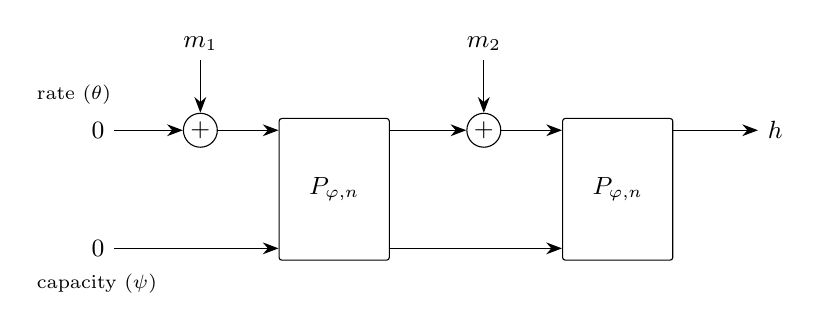
\begin{tikzpicture}[>={Stealth[length=2mm]}, font=\small,
  perm/.style={draw, rounded corners=1pt, minimum width=14mm, minimum height=18mm},
  add/.style={draw, circle, inner sep=1pt}]
  % initial state
  \node (r0) at (0, 1.5) {$0$};
  \node (c0) at (0, 0) {$0$};
  % absorb m1
  \node[add] (x1) at (1.3, 1.5) {$+$};
  \node (m1) at (1.3, 2.6) {$m_1$};
  % first permutation
  \node[perm] (p1) at (3.0, 0.75) {$P_{\varphi,n}$};
  % absorb m2
  \node[add] (x2) at (4.9, 1.5) {$+$};
  \node (m2) at (4.9, 2.6) {$m_2$};
  % second permutation
  \node[perm] (p2) at (6.6, 0.75) {$P_{\varphi,n}$};
  % output
  \node (hout) at (8.6, 1.5) {$h$};
  % rate wires
  \draw[->] (r0) -- (x1);
  \draw[->] (m1) -- (x1);
  \draw[->] (x1) -- (x1 -| p1.west);
  \draw[->] (p1.east |- x2) -- (x2);
  \draw[->] (m2) -- (x2);
  \draw[->] (x2) -- (x2 -| p2.west);
  \draw[->] (p2.east |- hout) -- (hout);
  % capacity wires
  \draw[->] (c0) -- (c0 -| p1.west);
  \draw[->] (p1.east |- c0) -- (c0 -| p2.west);
  % labels
  \node[anchor=west, font=\scriptsize] at (-0.9, 1.95) {rate ($\theta$)};
  \node[anchor=west, font=\scriptsize] at (-0.9, -0.45) {capacity ($\psi$)};
\end{tikzpicture}
\caption{The Mambo 2-to-1 sponge hash at $t = 2$ (rate~1,
capacity~1; Definition~\ref{def:sponge_hash}). The capacity lane is
never exposed: it is zero-initialised, passes only through the
permutation, and is discarded at squeeze time. At width $t \ge 3$
the rate lane carries $t-1$ cells, both message elements are
absorbed at once, and a single permutation call suffices.}
\label{fig:sponge}
\end{figure}

\begin{definition}[Mambo sponge hash]\label{def:sponge_hash}
Given messages $m_1, m_2 \in \Fp$:
\begin{enumerate}[nosep]
  \item Initialize: $(\theta, \psi) \gets (0, 0)$.
  \item Absorb $m_1$: $\theta \gets \theta + m_1$;
        $(\theta, \psi) \gets P_{\varphi,n}(\theta, \psi)$.
  \item Absorb $m_2$: $\theta \gets \theta + m_2$;
        $(\theta, \psi) \gets P_{\varphi,n}(\theta, \psi)$.
  \item Squeeze: output $\theta$.
\end{enumerate}
\end{definition}

R1CS cost depends on state width. At $t\!=\!2$ (rate 1, two permutation
calls per 2-to-1 hash), the theoretical count is $4n$; at the
recommended $n\!=\!82$ this is $328$~NL. At the $n\!=\!65$ minimum
cell, Circom 2.2.3 measures $259$ nonlinear constraints
(Table~\ref{tab:measured}), one below the theoretical $4n = 260$
because the capacity is zero-initialised, making the first
permutation call's round-1 squaring $\psi_0^2 = 0 \cdot 0$ a
constant that the compiler folds; the same structural fold applies at
every~$n$.
At wider state $t\!\ge\!3$ (rate $t\!-\!1$, single permutation call): $tn$.
Recommended 128-bit 2-to-1 hash costs: $165$~NL at $t\!=\!3, n\!=\!55$;
$172$~NL at $t\!=\!4, n\!=\!43$
(Table~\ref{tab:landscape}).



\subsection{PRNG Mode}\label{sec:inst:prng}

\begin{definition}[Mambo PRNG]\label{def:prng}
Given a secret seed $(\theta_0, \psi_0)$ and step parameter~$k$:
\begin{enumerate}[nosep]
  \item Apply $k$ Mambo steps.
  \item Extract: output $\theta_k + \psi_k \pmod{p}$.
  \item Repeat.
\end{enumerate}
R1CS cost: $2k$~NL per output. At $k=1$: 2~NL per output element.
\end{definition}

\paragraph{Security caveat.}
At $k=1$ with public output, additive extraction is broken
(Proposition~\ref{thm:k1attack}). The PRNG at $k=1$ is secure only when
output is a private ZK witness. For public output the analysis minimum
is $k \ge 65$ for 128-bit security; the recommended configuration is
$k = 82$ ($164$~NL per output), applying the margin rule of
Section~\ref{sec:security:parameters}.

\begin{conjecture}[Hidden Coupling Property]\label{conj:hcp}
For the Mambo PRNG with $k \ge 65$, the output sequence is computationally
indistinguishable from random over~$\Fp$.
\end{conjecture}

\begin{lemma}[HCP in the ideal-permutation model]\label{lem:hcp_from_prp}
Let $P_{\varphi,k}$ be the $k$-round Mambo permutation on $\Fp^2$ and
let $\mathrm{PRNG}_k$ be the Mambo PRNG of Definition~\ref{def:prng}
with step parameter~$k$. For any distinguisher~$\mathcal{D}$ making
$q$ output queries to $\mathrm{PRNG}_k$, there is a
permutation distinguisher~$\mathcal{B}$ of comparable running time
such that
\[
  \mathrm{Adv}^{\mathrm{HCP}}_{\mathcal{D}}(\lambda)
  \;\le\;
  \mathrm{Adv}^{\mathrm{perm}}_{\mathcal{B}}(\lambda)
  \;+\;
  \frac{q(q+1)}{2\,p^{2}},
\]
where $\mathrm{Adv}^{\mathrm{perm}}_{\mathcal{B}}$ denotes
$\mathcal{B}$'s advantage in distinguishing oracle access to
$P_{\varphi,k}$ from a uniformly random permutation on~$\Fp^2$. In
the ideal-permutation model the first term vanishes and the Mambo
PRNG output sequence is $\tfrac{q(q+1)}{2p^2}$-close to uniform
on~$\Fp$; for the concrete permutation, Design
Claim~\ref{claim:structural} asserts that the first term stays below
the target threshold at the recommended parameters with $k \ge 65$
(recommended $k = 82$; Section~\ref{sec:inst:prng}).
\end{lemma}

The proof is a standard three-hybrid argument (permutation switch,
birthday-plus-cycle-closure switch, exact uniformity of the sum
extraction) and is given in Appendix~\ref{app:structural}; the
second hybrid contributes $\binom{q}{2}/p^2$ for collisions plus
$q/p^2$ for the event that the random-permutation orbit of the seed
closes within $q$ steps.

\paragraph{Why the sum extraction.}
The reduction uses only that the extraction map
$f\!:\!\Fp^{2}\!\to\!\Fp,\;f(\theta,\psi)=\theta+\psi$ is balanced
(the pre-image of every output has size~$p$). Any balanced linear
extraction enjoys the same bound; the choice $f(\theta,\psi)=
\theta+\psi$ in Definition~\ref{def:prng} is for circuit economy
(the extraction is a linear combination and costs $0$ nonlinear
constraints; the $2k$~NL per output is the step cost alone), not
security.

The reduction in Lemma~\ref{lem:hcp_from_prp} extends verbatim to
Mambo-$t$ (Section~\ref{sec:inst:wider}): in the hybrid argument,
$\Fp^{2}$ is replaced by $\Fp^{t}$, the birthday term becomes
$q(q+1)/(2p^{t})$, and the sum-extraction balance argument
generalises to any balanced linear extraction $\Fp^{t}\to\Fp^{r}$
for rate $r\le t-1$. The lemma reduces HCP to a
permutation-distinguishing advantage without algebraic hypotheses on
the underlying permutation; the independent empirical evidence for
the structural plausibility of Design Claim~\ref{claim:structural}
and Conjecture~\ref{conj:cico}---the 34/34 and 62/62
eliminant-degree batteries---is collected in
Section~\ref{sec:security:evidence}.

\begin{corollary}[HCP redundancy]\label{cor:hcp_red}
Conjecture~\ref{conj:hcp} follows from
Lemma~\ref{lem:hcp_from_prp} in the ideal-permutation model and
need not be assumed independently.  The Mambo security argument
therefore rests on a single assumption
(Design Claim~\ref{claim:structural}, with falsifiable algebraic form
Conjecture~\ref{conj:cico}), occupying the same epistemic position
as the ideal-permutation assumptions underlying Keccak, Poseidon,
and Anemoi.
\end{corollary}




\subsection{Wider-State Variants ($t \ge 3$)}\label{sec:inst:wider}

The triangular coupling generalizes to any state width~$t \ge 2$.
Let $(x_1, \ldots, x_t) \in \Fp^t$. The Mambo-$t$ step applies
$t$ sequential squarings, each feeding into the next:
\begin{align*}
x_1' &= \varphi \cdot x_1 + x_t^2 + c_{r,1}, \\
x_i' &= \varphi \cdot x_i + (x_{i-1}')^2 + c_{r,i}
\quad \text{for } i = 2, \ldots, t.
\end{align*}

\begin{proposition}[ALFOM preservation under wider state]\label{prop:wider_alfom}
Mambo-$t$ achieves $\eta = \log_2(2^t)/t = 1.0$ for every $t \ge 2$.
Each step costs $t$~nonlinear constraints (one squaring per element)
while multiplying the algebraic degree by~$2^t$.
\end{proposition}

The non-telescoping property (Proposition~\ref{prop:nontelescoping})
extends directly to wider state.

\begin{corollary}[Non-telescoping at wider state]\label{cor:nontelescoping_wider}
For Mambo-$t$, $t \ge 2$, in the rate-1 sponge convention (capacity
zeroed at the input, first output coordinate fixed to~$\tau$) and with
$\varphi \ne 0$: the elimination ideal of the round system in the rate
input is principal, generated by an eliminant of degree exactly
$2^{t(n-1)} = D_I$ with leading coefficient $\varphi^{2^{t(n-1)}}$, and
parts (i)--(iii) of Proposition~\ref{prop:nontelescoping} hold verbatim
with these values.
\end{corollary}

\begin{proof}
The round system is triangular in the same variable order, so the
evaluation argument of Proposition~\ref{prop:nontelescoping}(i)
applies unchanged. For the degree and leading coefficient: in round~1
the chain of $t$ squarings from the zeroed capacity gives degrees
$1, 2, \ldots, 2^{t-1}$ and leading coefficients
$\varphi, \varphi^2, \ldots, \varphi^{2^{t-1}}$, and in every later
round each update has its top term from the single squaring
($2 \deg x_t^{(r-1)} = 2^{t(r-1)} > 2^{t(r-2)} = \deg x_1^{(r-1)}$ and
$2 \deg x_{i-1}^{(r)} > \deg x_i^{(r-1)}$ at every step), giving
$\deg x_1^{(n)} = 2^{t(n-1)}$ and
$\operatorname{lc}\, x_1^{(n)} = \varphi^{2^{t(n-1)}}$ by induction.
The discriminant argument of
Proposition~\ref{prop:nontelescoping}(iii) applies since
$p \nmid 2^{t(n-1)}$ for odd~$p$.
\end{proof}

\paragraph{Sponge CICO degree for wider state.}
For the sponge CICO problem with rate~$r=1$, capacity~$c=t-1$,
fixing $x_2(0) = \cdots = x_t(0) = 0$ and
$x_1(n) = \tau$, the univariate polynomial
$x_1(n)$ in the unknown $x_1(0)$ has formal degree
$D_I = 2^{t(n-1)}$ over the algebraic closure (the first round
consumes one factor of~$2^{(t-1)}$ because the initial capacity is
zero; subsequent rounds multiply by~$2^t$).
We verified $D_I = 2^{t(n-1)}$ computationally through $n = 5$ for
$t = 3, 4$ over $\F_{65521}$ and $\F_{1048573}$, with square-free
polynomial in all tested cases. Over $\Fp$ the effective bound is
$\min\!\bigl(2^{t(n-1)},\, p^{t}\bigr)$; the field-saturation
condition $t \log_2 p \ge \lambda$ determines which base fields admit
a given tier, as tabulated in Table~\ref{tab:field-applicability}.
The deployed capacity-1 hash surface at $t \ge 3$ additionally
admits the rate-specialization attack of
Section~\ref{sec:security:specialization}, which lowers the binding
eliminant degree to $D_{\mathrm{eff}} = 2^{t(n-1)-(t-2)}$; tier
sizing uses $D_{\mathrm{eff}}$, not the rate-1 figure above.

\paragraph{Rate--throughput summary.}
Mambo-$t$ at the recommended 128-bit cells (Table~\ref{tab:tiers})
achieves the following 2-to-1 sponge hash costs:
\begin{itemize}[nosep]
  \item $t\!=\!2, n\!=\!82$: rate $1$, two permutation calls, $328$~NL
        (at the minimum cell $n\!=\!65$: $260$~NL theoretical, $259$
        measured; Table~\ref{tab:measured}).
  \item $t\!=\!3, n\!=\!55$: rate $2$, one permutation call, $165$~NL.
  \item $t\!=\!4, n\!=\!43$: rate $3$, one permutation call, $172$~NL.
\end{itemize}
Each entry follows from $t$ nonlinear constraints per round times $n$ rounds
(Section~\ref{sec:map:r1cs}), multiplied by the number of permutation calls
required to absorb the two message elements at the given rate.



\subsection{Comparison Table}\label{sec:inst:comparison}

The constraint counts and figure of merit appear in
Table~\ref{tab:landscape} (Section~\ref{sec:intro:alfoms}).


%=============================================================================
\section{Implementation and Verification}\label{sec:implementation}
%=============================================================================

\subsection{Implementations}\label{sec:impl:systems}

Reference implementations are provided across the following back-ends.
All six produce bit-identical outputs against a common Python reference
on the test vectors of Appendix~\ref{app:testvectors}.

\begin{table}[h]
\centering
\caption{Reference implementations. All back-ends are tested,
cross-verified reference code; none has undergone an external
security audit, and ``tested'' should not be read as
production-hardened.}
\label{tab:implementations}
\small
\begin{tabular}{@{}llll@{}}
\toprule
Back-end & Field & Cost & Status \\
\midrule
Python (ref)        & multi             & ---                     & Specification \\
Circom (R1CS)~\cite{Circom}       & BN254             & $2n$                    & Constraint counting \\
Halo2 (Plonk/KZG)~\cite{PLONK,Halo2}   & BN254             & $2n$ custom gates       & Tested \\
Plonky3 (STARK/FRI)~\cite{Plonky3} & BB, KB, GL        & $2n$ AIR rows           & Tested \\
Noir / ACIR         & BN254             & $2n$ (custom gate: less) & Tested \\
Cairo~\cite{Cairo_Goldberg}               & Stark field       & $2n$                    & Tested \\
Stwo (Circle STARK) & Mersenne-31       & one perm / row          & Tested \\
\bottomrule
\end{tabular}
\smallskip

\footnotesize
BB = BabyBear, KB = KoalaBear, GL = Goldilocks. Plonky3 also supports a
one-permutation-per-row unrolled AIR variant.
\end{table}


\subsection{Performance}\label{sec:impl:performance}

The reference implementation produces the predicted constraint count
of Proposition~\ref{prop:cost} and runs at single-permutation cost
quoted below on commodity hardware. Comparison against existing
primitives at the design level (constraint count, ALFOM, R1CS cost)
is provided by Table~\ref{tab:landscape} in
Section~\ref{sec:intro:comparison}. The single-anchor number in
Table~\ref{tab:perf-anchor} fixes the predicted-cost match;
Appendix~\ref{app:extended-perf} reports the cross-system wall-clock
measurements at production proof depths, the UltraHonk custom-gate
arithmetisation, the Plonky3 recursive-verifier prove time across
round counts, and the Stwo Circle-STARK wider-state tier sweep.

\begin{table}[!htbp]
\centering
\caption{Reference single-permutation prove and verify time for Mambo
$t=2$ $n=65$ on Plonky3/FRI over BabyBear, release mode, reference
host. Configuration status: BabyBear fails the saturation condition
$t \log_2 p \ge \lambda$ at $t=2$
(Table~\ref{tab:field-applicability}), so this cell is not a
recommended tier; it is retained as the cross-system scaling anchor
because relative ratios across proof systems at matched $(t, n)$ are
the meaningful quantity, and absolute costs scale linearly in the
round count.}
\label{tab:perf-anchor}
\small
\begin{tabular}{@{}lrl@{}}
\toprule
Metric & Value & Unit \\
\midrule
Prove           & 12  & ms \\
Verify          & 1   & ms \\
NL constraints  & 130 & --- \\
\bottomrule
\end{tabular}
\smallskip

\footnotesize
Median of 11 runs on the reference Linux cloud VM (8-vCPU AMD, 16~GB
RAM); see Appendix~\ref{app:extended-perf} for the full cross-system
table and provenance. The constraint-count column matches
Proposition~\ref{prop:cost}.
\end{table}

\FloatBarrier


\subsection{Test Vectors and Cross-Verification}\label{sec:impl:testvectors}

Test vectors below are reproduced bit-identically by every back-end of
Section~\ref{sec:impl:systems}.

\begin{table}[h]
\centering
\caption{Step trace for $(\theta_0, \psi_0) = (1,1)$, $\varphi = 7$, BN254,
with round constants $c_i = d_i = 0$ (illustrative).}
\label{tab:steptrace}
\begin{tabular}{@{}rrl@{}}
\toprule
Step & $\theta_n$ & $\psi_n$ \\
\midrule
0 & 1 & 1 \\
1 & 8 & 71 \\
2 & 5\,097 & 25\,979\,906 \\
3 & 674\,955\,515\,804\,515 & 455\,564\,948\,314\,938\,897\,947\,876\,244\,567 \\
\bottomrule
\end{tabular}
\smallskip

\footnotesize
Production Mambo uses SHA-256-derived round constants
(Section~\ref{sec:map:constants}); test vectors with the production
constants are in Appendix~\ref{app:testvectors}.
\end{table}

Full 65-step test vectors for BN254, Goldilocks, and Mersenne-61 are
provided in Appendix~\ref{app:testvectors}.


\subsection{Measured Constraint Counts}\label{sec:impl:constraints}

\begin{table}[h]
\centering
\caption{Machine-measured R1CS constraint counts (Circom 2.2.3), at
the $t=2$ L1 minimum cell $n=65$ and $k=1$ PRNG; counts scale
linearly in the round count (e.g.\ $164/328$ at the recommended
$n=82$).}
\label{tab:measured}
\begin{tabular}{@{}lrrl@{}}
\toprule
Circuit & Theoretical & Measured & Status \\
\midrule
Permutation ($n=65$)  & 130 & 130 & Exact match \\
Sponge hash (2-to-1)  & 260 & 259 & One $0\!\cdot\!0$ squaring folded$^{\mathrm{f}}$ \\
PRNG (100 outputs)    & 200 & 200 & Exact match \\
\bottomrule
\end{tabular}
\smallskip

\footnotesize
$^{\mathrm{f}}$The deficit is exactly one constraint and is
structural: the sponge initialises the capacity to zero, so the
first permutation call's round-1 squaring $\psi_0 \cdot \psi_0$ is a
constant and Circom folds it. The count is identical at the default
and \texttt{-{}-O2} optimization levels. An earlier draft of this
table reported $255$, which we traced to a 2-to-1 sponge compiled at
$n = 64$ ($4 \cdot 64 - 1 = 255$); the figure above is the $n = 65$
measurement.
\end{table}


%=============================================================================
\section{Conclusion}\label{sec:conclusion}
%=============================================================================

We have introduced the Mambo map, a two-variable coupled quadratic
permutation over prime fields, and proved that its algebraic degree grows as
$4^n$ at R1CS cost~$2n$, matching the theoretical maximum
$\eta = 1.0$. Alongside Clotho ($\beta=2$) from~\cite{ALFOMs}, which was
introduced as a theoretical instance at this bound, Mambo is offered as
a complementary family accompanied by concrete instantiations and a
security study.

The core contribution is the exact algebraic characterization and its
proofs. The degree growth of~$4^n$ is a theorem
(Theorem~\ref{thm:degree}) with a constructive proof showing that no
cancellations occur at any step. This theorem and the $t=2$
closed-form regularity result $d_{\mathrm{reg}} = 2n$ are
machine-checked in Lean~4; the tier-floor Macaulay arithmetic is
kernel-verified, conditional on the measured $d_{\mathrm{reg}}$ at
$t \in \{3, 4\}$; the development is \texttt{sorry}-free, uses only
the three standard axioms (none for the floor computations), and is
provided as supplementary material. The formalisation verifies the
mathematics, not the attack-cost model. We have provided concrete
instantiations sized under the conservative cost model with a $25\%$
recommended round margin (sponge hash
at 165~NL at 128-bit with wider state $t\!=\!3$, $n\!=\!55$, or
172~NL at $t\!=\!4$, $n\!=\!43$; permutation at 164~NL for the
128-bit narrow state; PRNG at 2~NL per private-witness output) with
cross-verified
implementations in five proof systems.

The security of Mambo as a cryptographic primitive rests on a single
explicitly stated assumption: that the permutation admits no
structural distinguisher below the target cost at the recommended
parameters (Design Claim~\ref{claim:structural}), with the
CICO-hardness conjecture (Conjecture~\ref{conj:cico}) as its
falsifiable algebraic form. The conjecture is supported by the
explicit Gr\"obner-basis and eliminant analysis of
Section~\ref{sec:security}, differential analysis, and statistical
testing. We have self-disclosed the capacity-1 rate-specialization
attack, which costs $t-2$ bits at every wide state width and is
priced into every parameter row
(Section~\ref{sec:security:specialization}), self-disclosed a
polynomial-time attack on additive extraction at $k=1$
(Proposition~\ref{thm:k1attack}), disclosed all small-field
cryptanalysis results, and framed hash security via the BDPV08 sponge
indifferentiability theorem in the ideal-permutation model.

Several directions remain open. The relation
$d_{\mathrm{reg}} = 2n$ is now structurally established for all $n \ge 2$
(Theorem~\ref{thm:hilb_closed} in Appendix~\ref{app:dreg_proof}) via
an explicit Gr\"obner basis with pairwise coprime leading monomials
and Buchberger's first criterion; the value is one below the strict
semi-regularity prediction~$2n+1$, reflecting a single non-generic
syzygy in the CICO ideal that the proof identifies as the eliminated
$s_{n-1}$ relation. Reducing Conjecture~\ref{conj:cico} to a standard
computational assumption remains the most impactful open problem.

The question this paper raises is whether the algebraic efficiency
captured by $\eta = 1.0$ can coexist with cryptographic security. We
invite the community to investigate whether: (i)~Conjecture~\ref{conj:cico}
reduces to a standard computational assumption;
(ii)~the closed-form prediction of the higher Hilbert coefficients
beyond the first two---now \emph{resolved at $t = 4$}, where the
Hilbert series is $(1+z)^{4n-9} Q_4(z)$ with residue $Q_4 =
z^5 + 11 z^4 + 25 z^3 + 19 z^2 + 7 z + 1$ and $d_{\mathrm{reg}} = 4n-3$
for all $n \ge 4$ (Theorem~\ref{thm:t4_hilb}), the genericity of the
underlying leading-monomial set being certified by random
specialization---can be pushed to a fully deterministic
symbolic-constant confirmation, and whether the analogous
($n$-stable, septic) residue at widths $t \ge 5$ admits a closed form;
(iii)~further cryptanalysis of the coupled-quadratic structure reveals
any non-generic algebraic shortcut across the parameter ranges summarised
in Table~\ref{tab:landscape}; and (iv)~the $n \le t$ analysis gap can
be closed---regularity and specialization analysis at widths
$t \ge 5$---which is the named open problem whose resolution would
create the first recommended 128-bit configurations on 31-bit fields
(Section~\ref{sec:security:parameters}).

We close by restating the paper's framing as an explicit
cryptanalysis challenge, with the exact objects an attacker needs.
The falsification targets are the \emph{minimum} cells of
Table~\ref{tab:tiers} ($n = 65/44/34$ at $t = 2/3/4$ for
$\lambda = 128$), sized at exact analysis equality
$D_{\mathrm{eff}} = 2^{\lambda}$ with zero margin: any algebraic
solve of the capacity-1 CICO instance below
$\widetilde{O}(\min(D_{\mathrm{eff}}, p))$ at a minimum cell
falsifies Conjecture~\ref{conj:cico} outright, while the recommended
cells ($n = 82/55/43$) retain a $\ge 32$-bit buffer so that such a
result would not immediately translate to deployed parameters. The
attacker's toolkit is supplied in full: the explicit degrevlex
Gr\"obner basis of the CICO ideal (Appendix~\ref{app:dreg_proof}),
the closed-form Hilbert series and eliminant degrees
$D_I = 2^{t(n-1)}$ and $D_{\mathrm{eff}} = 2^{t(n-1)-(t-2)}$, the
SHA-256-derived round constants (Section~\ref{sec:map:constants}),
the reproducer scripts of the supplementary material, and the
self-disclosed attack surface (rate specialization, $k=1$
extraction, small-field artifacts). Sharper targets than a full
break are also stated: falsify the functional-indecomposability
hypothesis behind the monodromy certificates
(Section~\ref{sec:security:evidence}), beat the measured
$D_{\mathrm{eff}}$ specialization optimum at any cell, exhibit an
invariant structure escaping the classification of
Section~\ref{sec:security:spongelevel}, or close the multi-block
chaining-value question raised there in the attacker's favour. The
permutation, in short, is offered to the community with its
mathematics fully exposed and its weakest deliberate point marked.


%=============================================================================
\section*{Acknowledgments}
%=============================================================================

The author thanks Aur\'{e}lien Boeuf for feedback on fixed-point
structure, which motivated the introduction of per-round constants
(Section~\ref{sec:map:constants}); Pierre Briaud for the
correction of our initial $D_I$ estimate, which refined our security
analysis and clarified the applicability of the FreeLunch framework
(Section~\ref{sec:security:interpolation}); and H{\aa}vard Raddum for
the observation that the algebraic-degree argument must account for
finite-field saturation
(Section~\ref{sec:security:interpolation},
Table~\ref{tab:field-applicability}).

\section*{Intellectual Property Statement}

A provisional patent application covering the Mambo construction was
filed with the USPTO in March~2026 (patent pending). The reference
implementation, formal development, and reproduction scripts
accompanying this paper are released for research, academic
verification, and audit use; production and commercial use are
governed by the Business Source License~1.1 and the pending patent.
This statement is provided for transparency; nothing in it restricts the
reproduction or verification of the results reported here.


%=============================================================================
\appendix
%=============================================================================

\section{Reference Implementation}\label{app:reference}

The Mambo map in Python (reference):
\begin{verbatim}
import hashlib, struct

def derive_round_constants(n, p,
        seed=b"Mambo_round_constants"):
    vals = []
    for j in range(2 * n):
        h = hashlib.sha256(
            seed + j.to_bytes(4, "big")).digest()
        v = int.from_bytes(h, "big") % p
        vals.append(v if v != 0 else 1)
    return [(vals[i], vals[n + i])
            for i in range(n)]

def mambo_step(theta, psi, phi, c, d, p):
    theta_new = (phi * theta + psi * psi + c) % p
    psi_new   = (phi * psi
                 + theta_new * theta_new + d) % p
    return theta_new, psi_new

def mambo_permutation(theta, psi, phi, p, n=82):
    rc = derive_round_constants(n, p)
    for i in range(n):
        c_i, d_i = rc[i]
        theta, psi = mambo_step(
            theta, psi, phi, c_i, d_i, p)
    return theta, psi
\end{verbatim}

The sequential coupling is on line~17: \texttt{psi\_new} is a function of
\texttt{theta\_new}---the freshly computed~$\theta$---rather than of the input
\texttt{theta}. This is what forces the non-telescoping property
(Proposition~\ref{prop:nontelescoping}):
no round can be bypassed without solving both coupled constraints. Round constants are derived deterministically from
SHA-256 in counter mode.


\section{Extended Test Vectors}\label{app:testvectors}

All permutation test vectors below are pinned at $n = 65$ rounds (the
$t=2$ L1 minimum cell, the analysis anchor); pass \texttt{n=65}
explicitly when reproducing them. The recommended deployment round
count is $n = 82$ (Table~\ref{tab:tiers}).

\paragraph{BN254 scalar field.}
$\varphi = 7$. The BN254 scalar field prime is:

{\small
\begin{verbatim}
p = 2188824287183927522224640574525727508854836440
    0416034343698204186575808495617
\end{verbatim}
}

\noindent Permutation ($n = 65$, seed $(1, 1)$):

{\small
\begin{verbatim}
theta_65 = 1739473253535723036079722344930694285516
           1894228674458177983473076235044019007
psi_65   = 7276451156888393224863406760675751049923
           791015985763477840281348092940222991
\end{verbatim}
}

\paragraph{Goldilocks field.}
$p = 2^{64} - 2^{32} + 1 = 18446744069414584321$,
$\varphi = 7$.

\noindent Permutation ($n = 65$, seed $(1, 1)$):
\begin{align*}
\theta_{65} &= 14260991711422744827 \\
\psi_{65}   &= 4124660317069805710
\end{align*}


\section{R1CS Circuit for One Mambo Step}\label{app:r1cs}

A single Mambo step $(\theta_i, \psi_i) \to (\theta_{i+1}, \psi_{i+1})$
at round~$i$ with constants $(c_i, d_i)$:

Witness variables: $\theta_i, \psi_i, u_i, \theta_{i+1}, v_i, \psi_{i+1}$.

Constraints:
\begin{enumerate}[nosep]
  \item (Nonlinear)\quad $\psi_i \cdot \psi_i = u_i$
  \item (Linear)\quad $\varphi\cdot\theta_i + u_i + c_i = \theta_{i+1}$
  \item (Nonlinear)\quad $\theta_{i+1} \cdot \theta_{i+1} = v_i$
  \item (Linear)\quad $\varphi\cdot\psi_i + v_i + d_i = \psi_{i+1}$
\end{enumerate}

Total: 2~nonlinear constraints, 2~linear constraints. Only the nonlinear
constraints contribute to the cost~$C$. The round constants $c_i, d_i$
appear only in the linear constraints and add no nonlinear cost.


\section{Security Analysis Summary}\label{app:security_checklist}

Table~\ref{tab:security_checklist} summarizes all attack vectors analyzed
for the Mambo permutation and their current status.

\begin{table}[H]
\centering
\caption{Security analysis checklist for Mambo at the L1 minimum cell
($n=65$, $t=2$, BN254)---the falsification target of the cost model.
Every entry is monotone in the round count, so the recommended cell
($n=82$) inherits each status with margin.}
\label{tab:security_checklist}
\footnotesize
\begin{tabular}{@{}llll@{}}
\toprule
Attack Vector & Result & Section & Status \\
\midrule
Interpolation          & $D = 4^{65} \approx 2^{130}$ & \ref{sec:security:interpolation} & Secure \\
Gr\"obner basis (GB)   & basis explicit (free); Macaulay vs blind F4/F5 $> 2^{300}$ & \ref{sec:security:groebner} & See $D_I$ row \\
Ideal degree ($D_I$)   & $D_I = 4^{n-1} = 2^{128}$; univariate solve $\widetilde{O}(D_I)$ & \ref{sec:security:costmodel} & Secure \\
Higher-order diff.     & $\deg(\theta_{65}) = 2^{128}$ in sponge & \ref{sec:security:interpolation} & Secure at $n=65$ \\
Differential           & MDP $= 1/p$ per round (exact); trail $\le p^{-65}$ & \ref{sec:security:difflin} & Secure \\
Boomerang / BCT        & Max BCT $\le 6\times$ random; infeasible & \ref{sec:security:difflin} & Secure \\
Linear                 & Quadratic S-box, no high-bias trails & \ref{sec:security:difflin} & Secure \\
Slide attacks          & Round constants eliminate & \ref{sec:security:slide} & Secure \\
Invariant subspaces    & No invariant/trail lines at $t=2$ (complete); $t \ge 3$ partial & \ref{sec:security:spongelevel} & See section \\
Fixed points           & $\le 4$ per round; no common round fixed point & \ref{sec:security:spongelevel} & Analyzed \\
Multi-block CICO       & Chaining-value specialization unanalyzed & \ref{sec:security:spongelevel} & Open \\
$k=1$ additive attack  & Polynomial-time; recommended public-output $k = 82$ & \ref{sec:security:k1attack} & Disclosed \\
$c=1$ specialization ($t \ge 3$) & $D_{\mathrm{eff}} = 2^{t(n-1)-(t-2)}$; priced into tiers & \ref{sec:security:specialization} & Disclosed \\
Statistical tests      & PractRand 1\,TB, BigCrush 160/160 & \ref{sec:security:evidence} & Passed \\
\bottomrule
\end{tabular}
\end{table}


%=============================================================================
\section{Extended Performance Measurements}\label{app:extended-perf}
%=============================================================================

This appendix reports the proof-system-specific wall-clock and
proof-size data complementary to the single-anchor measurement of
Section~\ref{sec:impl:performance} (Table~\ref{tab:perf-anchor}).
All numbers are from the same reference Linux cloud VM (8-vCPU AMD,
16~GB RAM, Ubuntu 24.04) and the same bench harness; provenance,
commit hashes, and full p10/p50/p90 distributions are listed in the
supplementary materials.

\subsection{Single-permutation cost across proof systems}

\begin{table}[H]
\centering
\caption{Single-permutation Mambo performance at reference parameters,
release mode. Halo2 and Plonky3 figures are for the narrow $t=2$
$n=65$ permutation (the L1 minimum cell). UltraHonk gate counts are
for $t=4$ $n=18$
(the dense-FGLM-model L1 cell of Table~\ref{tab:tiers_fglm}; the
conservative L1 minimum cell at $t=4$ is $n=34$, recommended
$n=43$). KZG proof size is constant;
FRI grows with trace.}
\label{tab:perf-single}
\small
\begin{tabular}{@{}lrrrl@{}}
\toprule
Metric & Halo2/KZG & Plonky3/FRI & UltraHonk & Unit \\
\midrule
Prove         & 174 & 12  & --- & ms \\
Verify        & 13  & 1   & --- & ms \\
Proof size    & 960 & var & --- & B \\
Gates/perm    & --- & --- & 133 (std.) / \textbf{61} (custom) & gates \\
Trusted setup & Yes & No  & No  & --- \\
Post-quantum  & No  & Yes & No  & --- \\
\bottomrule
\end{tabular}
\end{table}

\paragraph{UltraHonk custom gate.}
A custom-gate extension to the UltraHonk arithmetisation reduces Mambo
$t=4$ $n=18$ to 61 UltraHonk gates per permutation, compared to 133 in
the default non-custom arithmetisation. The reduction is obtained by
consolidating the coupled-quadratic round into a single degree-2 gate
instance rather than separate squaring constraints.

\subsection{Halo2/KZG Merkle verifier prove time at production depths}

\begin{table}[H]
\centering
\caption{Halo2/KZG Merkle verifier prove time on BN254 at production
depths, Mambo $t=4$ $n=18$ (the dense-FGLM-model L1 cell of
Table~\ref{tab:tiers_fglm}). The local symbol
$\kappa$ denotes the KZG circuit-size parameter (trace domain size
$2^\kappa$); this is unrelated to the PRNG step parameter~$k$ of
Section~\ref{sec:inst:prng}.}
\label{tab:perf-merkle-halo2}
\small
\begin{tabular}{@{}rrr@{}}
\toprule
Depth & $\kappa$ & Prove (ms) \\
\midrule
10  & 9  & 367 \\
16  & 10 & 529 \\
20  & 10 & 596 \\
24  & 10 & 573 \\
64  & 12 & 908 \\
128 & 13 & 1313 \\
256 & 14 & 2411 \\
512 & 15 & 4300 \\
\bottomrule
\end{tabular}
\end{table}

\subsection{Plonky3/FRI production Merkle proof-size scaling}

\begin{table}[H]
\centering
\caption{Plonky3/FRI production Merkle verifier proof size for Mambo
$t=2$ $n=18$ (speed proxy). KoalaBear results within 2--5\% of BabyBear
at matched configuration. $n=18$ at $t=2$ is a speed-proxy
configuration for cross-depth scaling; the conservative 128-bit $t=2$
minimum cell is $n=65$, recommended $n=82$
(cf.\ Section~\ref{sec:security:parameters}). A
tier-secure wider-state Plonky3 Merkle verifier AIR is under
construction and will supersede this table when shipped.}
\label{tab:perf-plonky3-merkle}
\small
\begin{tabular}{@{}rrr@{}}
\toprule
Depth & Proof size (B) & Field \\
\midrule
2   &  27\,519 & BabyBear \\
4   &  30\,311 & BabyBear \\
8   &  39\,327 & BabyBear \\
16  &  51\,485 & BabyBear \\
64  &  85\,401 & BabyBear \\
128 & 107\,159 & BabyBear \\
512 & 160\,275 & BabyBear \\
\bottomrule
\end{tabular}
\end{table}

\subsection{Plonky3 recursive-verifier end-to-end prove time}

End-to-end recursive prove-time measurement on a Plonky3 FRI-only
recursive verifier at 32\,k rows on BabyBear, median of 11 trials with
p10 and p90 bands.

\begin{table}[H]
\centering
\caption{Plonky3 recursive verifier total prove time, Mambo. BabyBear
is sub-$L1$-secure at $t=2$ for any $n$; round counts shown are scaling
references. Empirical hash share of this FRI-only recursive verifier
on the tested round counts: 72--84\%, higher than typical
arithmetic-verifier-heavy recursive stacks because a pure FRI
recursive verifier is hash-dominated in its inner loop.}
\label{tab:perf-plonky3-recursive}
\small
\begin{tabular}{@{}lrr@{}}
\toprule
Configuration & Median (ms) & p10--p90 (ms) \\
\midrule
Mambo $t=4$ $n=18$  &  744 & 715--858 \\
Mambo $t=2$ $n=33$  &  715 & 687--785 \\
Mambo $t=2$ $n=49$  &  905 & 870--985 \\
Mambo $t=2$ $n=65$  & 1155 & 1120--1215 \\
\bottomrule
\end{tabular}
\end{table}

The recursive-verifier measurements are prove-cost measurements and
field-independent; they apply at any $t=2$-admissible field at the
same round counts. Tier-level security labels are omitted here
because the underlying field is BabyBear, for which the
field-saturation condition of
Section~\ref{sec:security:parameters} caps accessible security below
$L1$ at $t=2$ regardless of $n$.

\subsection{Stwo (Circle STARK, Mersenne-31)}

Mambo runs natively in the Circle STARK framework underlying Stwo at
all state widths tested ($t \in \{2, 16, 32\}$) because the
permutation has constraint degree exactly $2$ by construction. The
framework enforces a degree-$2$ upper bound on constraint polynomials
in its present form; primitives whose rounds have algebraic degree
above~$2$ require auxiliary witness columns to be represented under
this ceiling, while Mambo fits it natively.

\begin{table}[H]
\centering
\caption{Stwo prove time at $\log_n = 14$ (16\,384 parallel
permutations), median of five runs, reference host. The
$t \in \{16, 32\}$ widths are \emph{research configurations ---
insecure-until-analyzed}: they lie in the $n \le t$ regime for which
no regularity or specialization analysis exists
(Section~\ref{sec:security:parameters}), so no tier label or
security claim attaches to any row. Round counts were fixed purely
as reference points by the pre-specialization rule
$D_I = 2^{t(n-1)} \ge
2^{\lambda}$ for $\lambda \in \{128, 192, 256\}$: $n_{128} = 9$ at
$t=16$ and $n_{128} = 5$ at $t=32$;
$n_{192} = 13$ at $t=16$ and $n_{192} = 7$ at $t=32$;
$n_{256} = 17$ at $t=16$ and $n_{256} = 9$ at $t=32$. Under the
rate-specialization correction $D_{\mathrm{eff}} \ge 2^{\lambda}$
(Section~\ref{sec:security:specialization}) each reference round
count rises by exactly one ($t=16$: $n = 10/14/18$; $t=32$:
$n = 6/8/10$);
the measured times below are per-round-count references only,
and cross-configuration relative ratios are the meaningful quantity.}
\label{tab:perf-stwo}
\small
\begin{tabular}{@{}lrr@{}}
\toprule
Round count (reference only) & $t = 16$ (ms) & $t = 32$ (ms) \\
\midrule
$n_{128}$ & 453 & 806 \\
$n_{192}$ & 533 & 981 \\
$n_{256}$ & 794 & 882 \\
\bottomrule
\end{tabular}
\end{table}

Two scoping notes apply to these wide-width cells. First, sponge
collision resistance is bounded by $p^{c/2}$, so on a 31-bit field
the 128-bit collision level requires capacity
$c \ge \lceil 2 \cdot 128 / 31 \rceil = 9$ cells; the usable rate on
M31 is therefore $t - 9$, not $t - 1$ (rate $7$ at $t = 16$, rate
$23$ at $t = 32$). At the corrected reference round counts this gives
$160/7 \approx 22.9$ nonlinear constraints per absorbed element at
$t = 16$, $n = 10$, and $192/23 \approx 8.3$ at $t = 32$, $n = 6$; a
2-to-1 node over two 9-cell digests (18 cells) fits in a single
$t = 32$ permutation call ($192$ nonlinear constraints), while
$t = 16$ requires three calls. Second---the reason for the
research-configuration label---the wide-width cells lie in
the $n \le t$ regime, entirely outside the analyzed range of the
regularity and specialization measurements (the
$D_{\mathrm{eff}}$ closed form was measured at $t \in \{3, 4, 5\}$,
$n \in \{2, \ldots, 5\}$;
Section~\ref{sec:security:specialization}), and no recommended
128-bit configuration currently exists on 31-bit fields
(Section~\ref{sec:security:parameters}). We flag the
$t \in \{16, 32\}$ configurations as the priority target for further
cryptanalysis; closing the $n \le t$ analysis gap is the named open
problem of Section~\ref{sec:conclusion}.


%=============================================================================
\section{Structural Observations and Deferred Proofs}\label{app:structural}
%=============================================================================

\begin{remark}[First syzygy module is exactly Koszul]\label{rem:first_syz_koszul}
Computation of the minimal free resolution of the CICO ideal (via the
same \texttt{syzygy\_hunt\_sage} scripts) shows that the first syzygy
module coincides with the Koszul complex at every tested $n$: the
non-genericity reflected by Corollary~\ref{cor:hilbseries_closedform}
is not visible at the level of pairwise relations among the generators.
Homogenizing the ideal by introducing an auxiliary degree-$1$ variable
$h$ restores the semi-regular numerator $(1+z)^{2n}$ exactly, confirming
that the observed density gap is a purely affine phenomenon arising
from the interaction of the two degree-$1$ CICO endpoint constraints
with the $2n$ degree-$2$ propagation equations.
\end{remark}

\begin{remark}[Joint origin of the half-density and $1/p$ signals]\label{rem:joint_signal}
Two near-tight non-genericity observations on the Mambo round map admit a
common structural explanation:
\begin{enumerate}[nosep]
  \item Corollary~\ref{cor:hilbseries_closedform}:
    $\operatorname{hilb}(G,2) = (1+z)^{2n-1}$, one factor of $(1+z)$ shorter
    than the semi-regular baseline $(1+z)^{2n}$.
  \item Proposition~\ref{prop:mdp}: the maximum differential
    probability per round equals $1/p$, half the $2/p$ generic upper bound
    for a degree-$2$ permutation on~$\Fp^2$.
\end{enumerate}
Both observations are consistent with a single structural property of the
round map, which we term its \emph{bilinear-quadratic asymmetry}: the
output coordinate $\theta'$ depends on $\theta$ affinely and on $\psi$
quadratically, while $\psi'$ depends on $\psi$ affinely and on $\theta'$
quadratically. Each output coordinate depends on its ``own'' input
variable affinely and on the cross variable quadratically.

\emph{Algebraic side (signal 1).} Under homogenization, the leading forms
at infinity factor through one variable per equation: $\theta_{i+1} =
\psi_i^2$, $\psi_{i+1} = \theta_{i+1}^2$. The bilinear-quadratic asymmetry
is therefore present in the ideal of leading forms; the closed-form
factorization $(1+z)^{2n-1}$ of $\operatorname{hilb}(G,2)$ is empirically
observed for $n \in \{2,\dots,10\}$ (Corollary~\ref{cor:hilbseries_closedform})
and is consistent with this leading-form bilinearity. A formal derivation
of the factorization from the leading-form ideal is open work; we record
the structural connection here as the most parsimonious explanation
compatible with the data and the Koszul syzygy observation
(Remark~\ref{rem:first_syz_koszul}).

\emph{Differential side (signal 2).} The case analysis in the proof of
Proposition~\ref{prop:mdp} shows that every DDT row is either
concentrated in a single output column with $p$ preimages per cell
(input differences $(a, 0)$), or assigns $p$ preimages to exactly one
cell and one preimage to the rest (input differences with
$\Delta\psi \ne 0$). In both witness families the affine dependence on
the ``own'' variable is what forces the concentration, and the
quadratic dependence on the cross variable is what spreads the
remainder uniformly---the same asymmetry as on the algebraic side.

The bilinear-quadratic asymmetry is intentional: it minimizes nonlinear
constraint count (one squaring per output coordinate per round) and is
the source of the half-pack and quarter-pack circuit savings reported in
Section~\ref{sec:impl:performance}.
\end{remark}

\subsection*{Proof of Lemma~\ref{lem:hcp_from_prp}}\label{app:hcp_proof}

\begin{proof}
Let $(\theta_0,\psi_0)\sim\mathcal U(\Fp^{2})$ denote a uniformly random
seed and write the PRNG output $\sigma_i=\theta_{ki}+\psi_{ki}\pmod p$
where $(\theta_{ki},\psi_{ki})=P_{\varphi,k}^{\,i}(\theta_0,\psi_0)$ is
the $i$-th iterate of $P_{\varphi,k}$ on the seed.

\paragraph{Hybrids.}
Define three games, each producing a transcript
$(\sigma_1,\dots,\sigma_q)\in\Fp^{q}$:
\begin{itemize}[nosep]
  \item $\mathbf{H}_{0}$: real PRNG. Permutation $=P_{\varphi,k}$;
        $\sigma_i=(\theta_{ki}+\psi_{ki})$ as above.
  \item $\mathbf{H}_{1}$: $P_{\varphi,k}$ replaced by a uniform random
        permutation $\pi\!:\!\Fp^{2}\!\to\!\Fp^{2}$. Output
        $\sigma_i=a_i+b_i$ where $(a_i,b_i)=\pi^{i}(\theta_0,\psi_0)$.
  \item $\mathbf{H}_{2}$: $\pi$-orbit replaced by $q$ i.i.d.\ uniform
        samples $(u_i,v_i)\sim\mathcal U(\Fp^{2})$. Output
        $\sigma_i=u_i+v_i$.
\end{itemize}

\paragraph{Step 1: $\mathbf{H}_0\!\to\!\mathbf{H}_1$ (permutation switch).}
Given $\mathcal D$ distinguishing $\mathbf{H}_0$ from $\mathbf{H}_1$
with advantage~$\varepsilon_{01}$, build a permutation distinguisher
$\mathcal B$ as follows: $\mathcal B$ samples
$(\theta_0,\psi_0)\!\sim\!\mathcal U(\Fp^{2})$ and maintains a state
variable $s_0=(\theta_0,\psi_0)$.  For
$i=1,\dots,q$, $\mathcal B$ queries its permutation oracle on $s_{i-1}$ to
obtain $s_i$, records $\sigma_i$ as the sum of coordinates of $s_i$,
and feeds $\sigma_i$ to $\mathcal D$.  When $\mathcal D$ halts with a
guess, $\mathcal B$ outputs the same guess. If the oracle is
$P_{\varphi,k}$ (resp.\ a random permutation), $\mathcal B$ simulates
$\mathbf{H}_0$ (resp.\ $\mathbf{H}_1$) perfectly. Hence
$\varepsilon_{01}\le\mathrm{Adv}^{\mathrm{perm}}_{\mathcal B}(\lambda)$.
$\mathcal B$ runs in time $\mathrm{time}(\mathcal D)+q\cdot
\mathrm{cost}(\text{1 oracle query})$ and uses $q$ forward queries.

\paragraph{Step 2: $\mathbf{H}_1\!\to\!\mathbf{H}_2$ (birthday switch).}
Let $E$ be the event that the $\pi$-orbit of the seed closes within
the first $q$ steps, i.e.\ $\pi^{i}(\theta_0,\psi_0) =
(\theta_0,\psi_0)$ for some $1 \le i \le q$. Since the cycle length
of a uniformly random point under a uniformly random permutation of
a domain of size $p^2$ is uniform on $\{1, \ldots, p^2\}$,
$\Pr[E] \le q/p^{2}$. Conditioned on $\lnot E$, the orbit
$(a_1,b_1),\dots,(a_q,b_q)$ is
distributed as $q$ uniformly random \emph{distinct} points of
$\Fp^{2}$. The total variation distance between this distribution
and~$\mathcal U(\Fp^{2})^{q}$ (i.i.d.\ uniform samples) is bounded by
the probability of collision among~$q$ i.i.d.\ samples on a domain of
size~$p^{2}$. Adding the cycle-closure term,
\[
  \Delta\bigl(\mathbf H_1^{(a,b)},\,\mathbf H_2^{(a,b)}\bigr)
  \;\le\;\binom{q}{2}\Big/\,p^{2} \;+\; \frac{q}{p^{2}}
  \;=\;\frac{q(q+1)}{2\,p^{2}}.
\]
The transcript $(\sigma_i)_i$ is a deterministic post-processing of
$(a_i,b_i)_i$; by the data-processing inequality this bound transfers
to the distinguisher's view.

\paragraph{Step 3: $\mathbf{H}_2$ is uniform.}
For independent $u,v\!\sim\!\mathcal U(\Fp)$, the sum $u+v\bmod p$ is
distributed as~$\mathcal U(\Fp)$. The samples in~$\mathbf{H}_2$ are
mutually independent, so $\mathbf{H}_2$ produces $q$ i.i.d.\ uniform
elements of~$\Fp$.  Hence $\mathcal D$'s advantage in distinguishing
$\mathbf{H}_2$ from a uniform reference equals zero.

Combining the three steps via the triangle inequality yields the
claimed bound.
\end{proof}


%=============================================================================
\section{Structural Proof of $d_{\mathrm{reg}} = 2n$ via an Explicit Gr\"obner Basis}\label{app:dreg_proof}
%=============================================================================

This appendix upgrades the empirical observation $\operatorname{hilb}(G,2)
= (1+z)^{2n-1}$ (Corollary~\ref{cor:hilbseries_closedform}, verified
bit-exact through $n = 10$) to a theorem by exhibiting an explicit
Gr\"obner basis of the Mambo CICO ideal whose leading monomials are
pairwise coprime. The proof has two ingredients: (i) a
square-reduction lemma collapsing every free variable's square to a
linear polynomial in free variables; (ii) an explicit list of $2n+2$
ideal elements whose leading monomials are powers of distinct
variables, so Buchberger's first criterion gives the Gr\"obner basis
property without any explicit $S$-pair reduction. The standard
monomials read directly off the leading-monomial structure as the
squarefree monomials in a $(2n-1)$-element set, giving Hilbert series
$(1+z)^{2n-1}$ and $d_{\mathrm{reg}} = 2n$ for all $n \ge 2$.

Throughout this appendix we use the shorthand $t_i := \theta_i$ and
$s_i := \psi_i$ to match the variable-ordering convention of the
Singular reproducer
\texttt{analysis/mambo\_proof\_verify.sage}, which independently
verifies every algebraic identity below at $n \in \{2, 3, 4, 5, 6\}$
over $\F_{257}$.

\subsection{Setup}\label{app:dreg:setup}

Let $R = \F_p[t_0, t_1, \ldots, t_n, s_0, s_1, \ldots, s_n]$ with
$N = 2(n+1)$ variables. Let $I \subseteq R$ be the Mambo CICO ideal
at state width $t = 2$ and round count $n$, generated by the $2n+2$
polynomials
\begin{align*}
g_0  &:= t_0,
& g_{2n+1}  &:= t_n - \tau,\\
g_{2i+1} &:= t_{i+1} - \varphi t_i - s_i^2 - c_i,
& g_{2i+2} &:= s_{i+1} - \varphi s_i - t_{i+1}^2 - d_i,
\end{align*}
for $i = 0, 1, \ldots, n - 1$, where $\tau \in \F_p$ is the rate
output target, $\varphi \in \F_p^\ast$ is the multiplier, and
$(c_i, d_i)_{i = 0}^{n-1}$ are the round constants.

\subsection{Free variables and the candidate basis}\label{app:dreg:basis}

Define the \emph{free variable set}
\[
\mathcal{F}_n
:= \{ t_1, t_2, \ldots, t_{n-1} \}
\cup \{ s_0, s_1, \ldots, s_{n-2} \}
\cup \{ s_n \}
\]
and the \emph{fixed variable set}
$\mathcal{X}_n := \{ t_0, t_n, s_{n-1} \}$.
Note $|\mathcal{F}_n| = 2n - 1$ and $|\mathcal{X}_n| = 3$, so
$|\mathcal{F}_n| + |\mathcal{X}_n| = 2n + 2 = N$.

Let $\mathcal{B}_n$ denote the set of squarefree monomials in
$\mathcal{F}_n$:
\[
\mathcal{B}_n = \biggl\{ \prod_{x \in S} x \;:\; S \subseteq \mathcal{F}_n \biggr\},
\qquad
|\mathcal{B}_n| = 2^{|\mathcal{F}_n|} = 2^{2n-1}.
\]

\subsection{Reduction relations}\label{app:dreg:reductions}

Each fixed variable in $\mathcal{X}_n$ is reducible modulo the
generators of $I$:
\begin{align}
t_0       &\equiv 0 \pmod{I}, \tag{R1}\label{eq:appR1}\\
t_n       &\equiv \tau \pmod{I}, \tag{R2}\label{eq:appR2}\\
s_{n-1}   &\equiv \varphi^{-1} (s_n - \tau^2 - d_{n-1}) \pmod{I},
\tag{R3}\label{eq:appR3}
\end{align}
where (R3) is obtained from $g_{2n} = s_n - \varphi s_{n-1} - t_n^2 -
d_{n-1}$ combined with~\eqref{eq:appR2}.

\begin{lemma}[Square reduction]\label{lem:sq_reduction}
For every $x \in \mathcal{F}_n$, there exist scalars $a_y \in \F_p$
($y \in \mathcal{F}_n$) and $a_0 \in \F_p$ such that
\[
x^2 \equiv a_0 + \sum_{y \in \mathcal{F}_n} a_y \, y \pmod{I}.
\]
\end{lemma}

\begin{proof}
We treat the four cases.

\medskip
\noindent\emph{Case $x = s_i$, $i \in \{0, 1, \ldots, n-2\}$.}
Generator $g_{2i+1} = t_{i+1} - \varphi t_i - s_i^2 - c_i \in I$
gives $s_i^2 \equiv t_{i+1} - \varphi t_i - c_i \pmod{I}$. Both
$t_i$ and $t_{i+1}$ lie in $\mathcal{F}_n \cup \{t_0\}$; using
\eqref{eq:appR1} when $i = 0$, the right-hand side reduces to a linear
polynomial in $\mathcal{F}_n$.

\medskip
\noindent\emph{Case $x = t_i$, $i \in \{1, 2, \ldots, n-2\}$.}
The generator $g_{2i} = s_i - \varphi s_{i-1} - t_i^2 - d_{i-1} \in I$
gives $t_i^2 \equiv s_i - \varphi s_{i-1} - d_{i-1} \pmod{I}$. Both
$s_{i-1}$ and $s_i$ lie in $\mathcal{F}_n$ since $i - 1 \geq 0$ and
$i \leq n - 2$.

\medskip
\noindent\emph{Case $x = t_{n-1}$.}
The same generator $g_{2(n-1)} = s_{n-1} - \varphi s_{n-2} -
t_{n-1}^2 - d_{n-2}$ gives $t_{n-1}^2 \equiv s_{n-1} - \varphi
s_{n-2} - d_{n-2} \pmod{I}$. Now $s_{n-1} \in \mathcal{X}_n$, but
\eqref{eq:appR3} reduces $s_{n-1}$ to $\varphi^{-1} (s_n - \tau^2 -
d_{n-1})$, a linear polynomial in $\mathcal{F}_n$.

\medskip
\noindent\emph{Case $x = s_n$.}
Combine $g_{2n}$ with~\eqref{eq:appR2} to obtain
$s_{n-1} \equiv \varphi^{-1}(s_n - \tau^2 - d_{n-1}) \pmod{I}$.
Squaring,
$s_{n-1}^2 \equiv \varphi^{-2} (s_n - \tau^2 - d_{n-1})^2 \pmod{I}$.
Independently, $g_{2n-1} = t_n - \varphi t_{n-1} - s_{n-1}^2 - c_{n-1}$
combined with~\eqref{eq:appR2} gives
$s_{n-1}^2 \equiv \tau - \varphi t_{n-1} - c_{n-1} \pmod{I}$.
Equating the two expressions for $s_{n-1}^2$ and solving for $s_n^2$:
\[
s_n^2 \equiv 2(\tau^2 + d_{n-1}) s_n - \varphi^3 t_{n-1}
+ \bigl(\varphi^2(\tau - c_{n-1}) - (\tau^2 + d_{n-1})^2\bigr)
\pmod{I},
\]
which is linear in $\{s_n, t_{n-1}\} \subseteq \mathcal{F}_n$.
\end{proof}

\subsection{Spanning and linear independence}\label{app:dreg:basis_proof}

\begin{proposition}[$\mathcal{B}_n$ spans $R/I$]\label{prop:span}
The classes $\{\bar m : m \in \mathcal{B}_n\}$ span $R/I$ as an
$\F_p$-vector space.
\end{proposition}

\begin{proof}
Every monomial $m \in R$ is, by Lemma~\ref{lem:sq_reduction} and
relations \eqref{eq:appR1}--\eqref{eq:appR3}, congruent modulo $I$ to a
polynomial in the variables of $\mathcal{F}_n$ in which each variable
appears to power at most $1$. Such a polynomial is an
$\F_p$-linear combination of monomials in $\mathcal{B}_n$. Hence
$\mathcal{B}_n$ spans $R/I$.
\end{proof}

\begin{proposition}[$\mathcal{B}_n$ is linearly independent]\label{prop:indep}
The classes $\{\bar m : m \in \mathcal{B}_n\}$ are $\F_p$-linearly
independent in $R/I$.
\end{proposition}

\begin{proof}
We exhibit an explicit Gr\"obner basis $\mathcal{G}$ of $I$ under
the degrevlex order with variable ranking $t_0 > t_1 > \cdots >
t_n > s_0 > s_1 > \cdots > s_n$, and read off the standard monomials.

\medskip
\noindent\textbf{The candidate basis $\mathcal{G}$.} Define the
following $2n+2$ polynomials.
\begin{enumerate}[label=(G\arabic*),leftmargin=*]
\item    $\gamma_0 := t_0$.
    Leading monomial $t_0$.
\item    $\gamma_{2n+1} := t_n - \tau$.
    Leading monomial $t_n$.
\item $\rho := s_{n-1} - \varphi^{-1}(s_n - \tau^2 - d_{n-1})$.
    Leading monomial $s_{n-1}$.
\item For $i \in \{0, 1, \ldots, n-2\}$,
    $\eta_i := s_i^2 - (t_{i+1} - \varphi t_i - c_i)$.
    Leading monomial $s_i^2$.
\item For $i \in \{1, 2, \ldots, n-1\}$,
    $\kappa_i := t_i^2 - (s_i - \varphi s_{i-1} - d_{i-1})$.
    Leading monomial $t_i^2$.
\item  $\sigma :=
    s_n^2 - 2(\tau^2 + d_{n-1}) s_n + \varphi^3 t_{n-1}
    - \bigl(\varphi^2(\tau - c_{n-1}) - (\tau^2 + d_{n-1})^2\bigr)$.
    Leading monomial $s_n^2$.
\end{enumerate}
Set $\mathcal{G} := \{\gamma_0, \gamma_{2n+1}, \rho\} \cup
\{\eta_i\}_{i=0}^{n-2} \cup \{\kappa_i\}_{i=1}^{n-1} \cup
\{\sigma\}$. Then $|\mathcal{G}| = 3 + (n-1) + (n-1) + 1 = 2n + 2$.

\medskip
\noindent\textbf{Step 1: $\mathcal{G} \subseteq I$.}
$\gamma_0 = g_0 \in I$ and $\gamma_{2n+1} = g_{2n+1} \in I$ directly.
$\eta_i = -g_{2i+1} \in I$ for $i \leq n-2$. $\kappa_i = -g_{2i} \in I$
for $i = 1, \ldots, n-1$. For $\rho$: from $g_{2n} = s_n - \varphi s_{n-1}
- t_n^2 - d_{n-1}$ and $\gamma_{2n+1} = t_n - \tau$, we have
$\varphi \rho = -g_{2n} - (t_n + \tau) \gamma_{2n+1}$, so
$\varphi \rho \in I$, hence $\rho \in I$. For $\sigma$: by
Lemma~\ref{lem:sq_reduction} (case $x = s_n$), $s_n^2$ reduces to the
displayed linear polynomial in $\{s_n, t_{n-1}\}$ modulo $I$,
so $\sigma \in I$.

\medskip
\noindent\textbf{Step 2: $\mathcal{G}$ generates $I$.}
The original generators $\{g_0, g_{2n+1}\} \cup \{g_{2i+1}\}_{i=0}^{n-1}
\cup \{g_{2i+2}\}_{i=0}^{n-1}$ all lie in $\langle \mathcal{G} \rangle$:
$g_0 = \gamma_0$, $g_{2n+1} = \gamma_{2n+1}$, $g_{2i+1} = -\eta_i$ for
$i \leq n-2$, $g_{2i+2} = -\kappa_{i+1}$ for $i \leq n-2$. The
remaining two original generators, $g_{2n-1}$ and $g_{2n}$, follow:
$g_{2n} = -\varphi \rho - (t_n + \tau)\gamma_{2n+1}$ as above; and
$g_{2n-1}$ is recovered from $\sigma$, $\gamma_{2n+1}$, and $\rho$ by
the same closure derivation as in Lemma~\ref{lem:sq_reduction}. Hence
$\langle \mathcal{G} \rangle = I$.

\medskip
\noindent\textbf{Step 3: leading monomials of $\mathcal{G}$ are
pairwise coprime.}
The set of leading monomials is
\[
\mathrm{LM}(\mathcal{G}) = \{ t_0,\ t_n,\ s_{n-1} \} \cup
\{ s_i^2 \}_{i=0}^{n-2} \cup \{ t_i^2 \}_{i=1}^{n-1} \cup \{ s_n^2 \}.
\]
Each entry is supported on a single variable, and the variables are
distinct. Therefore $\gcd(m_1, m_2) = 1$ for every pair $m_1 \neq m_2$
in $\mathrm{LM}(\mathcal{G})$.

\medskip
\noindent\textbf{Step 4: $\mathcal{G}$ is a Gr\"obner basis of $I$.}
By Buchberger's first criterion (coprime leading monomials imply
trivial $S$-pair reduction; cf.\ Cox--Little--O'Shea
\emph{Ideals, Varieties, and Algorithms}, Thm.~3.6.4), pairwise coprime
leading monomials of generators that span $I$ imply that the
generators form a Gr\"obner basis of $I$. By Steps~1--3, $\mathcal{G}$
satisfies the hypotheses, hence $\mathcal{G}$ is a Gr\"obner basis of
$I$ under the chosen monomial order.

\medskip
\noindent\textbf{Step 5: standard monomials $= \mathcal{B}_n$.}
Macaulay's theorem identifies $R/I$ with the $\F_p$-vector space
spanned by monomials not divisible by any element of
$\mathrm{LM}(\mathcal{G})$. A monomial $m \in R$ avoids
$\mathrm{LM}(\mathcal{G})$ iff (a) $m$ is not divisible by $t_0$,
$t_n$, or $s_{n-1}$, and (b) $m$ is not divisible by any of
$s_0^2, \ldots, s_{n-2}^2, t_1^2, \ldots, t_{n-1}^2, s_n^2$. The first
condition restricts $m$ to monomials supported on
$\mathcal{F}_n = \{t_1, \ldots, t_{n-1}, s_0, \ldots, s_{n-2}, s_n\}$.
The second restricts those to squarefree monomials. The intersection
is exactly $\mathcal{B}_n$. The standard monomials are an $\F_p$-basis
of $R/I$, so the classes $\{\bar m : m \in \mathcal{B}_n\}$ are
linearly independent.
\end{proof}

\subsection*{The $t = 4$ residue: leading-monomial
classification}\label{app:dreg:t4}

The $t = 4$ closed form of Theorem~\ref{thm:t4_hilb} rests on an
explicit classification of the initial ideal. Unlike the $t = 2$ case,
the quotient is not a Boolean ring: the residue factor $Q_4(z) =
z^5 + 11 z^4 + 25 z^3 + 19 z^2 + 7 z + 1$ records a fixed finite set of
non-Boolean leading monomials that survive the Gr\"obner reduction.

\begin{lemma}[$t = 4$ leading-monomial classification, $n \ge 4$]\label{lem:t4_lm_classification}
For the rate-fixed CICO ideal $I$ at width $t = 4$ and every $n \ge 4$,
the degree-reverse-lex (round-major) initial ideal is exactly the
finite monomial certificate
$\operatorname{in}_<(I) = C$, where $C$ is generated by:
\begin{enumerate}[nosep]
  \item[(a)] six \emph{linear} monomials: the three input pins and the
    anti-diagonal linear chain $x_{n,0}, x_{n-1,1}, x_{n-2,2}$;
  \item[(b)] the \emph{Boolean square} $x^2$ of every other free
    variable;
  \item[(c)] a fixed finite \emph{non-Boolean certificate} of $57$
    monomials: the single tower $w^6$ with $w = x_{n,3}$, and $56$
    mixed monomials of the form $w^a \cdot u$ with $u$ a squarefree
    monomial on the nine-variable window of rounds $n-3, \ldots, n$.
\end{enumerate}
\end{lemma}

\begin{proof}
\emph{Window-local membership.} Define the four-round window subideal
$J_n \subseteq I$ generated by the round-map relations on rounds
$n-4 \to \cdots \to n$ together with the output pin; $J_n$ involves
only the state variables of those rounds. A direct (finite,
$n$-independent) computation verifies, at $n \in \{4,5,6,7\}$, that
every monomial of the certificate~(c) and every linear monomial
of~(a) is divisible by a leading monomial of a Gr\"obner basis of
$J_n$; hence for each certificate monomial $\mu$ there is $h \in J_n
\subseteq I$ with $\operatorname{LM}(h) \mid \mu$, so
$(\mu / \operatorname{LM}(h))\,h \in I$ has leading monomial exactly
$\mu$ and $\mu \in \operatorname{in}_<(I)$. The Boolean squares of~(b)
are leading monomials of the original round-map generators directly.
The window bound~$4$ is minimal: a three-round window fails to capture
the certificate monomials engaging round $n-3$.

\emph{$n$-uniformity.} In window coordinates the generators of $J_n$
are, for every $n$, the same polynomials up to the values of the
round constants, which the round-index shift merely re-indexes; the
monomial order restricts to the window with the relative order
preserved, so a window element with a given leading monomial maps under
the shift to one of $J_{n'}$ with the shifted leading monomial,
\emph{provided membership is independent of the constants}. We
establish constant-independence by upper-semicontinuity of the initial
ideal: regarding $J$ as a family over the parameter space of round
constants, $\operatorname{in}_<(J_v) \supseteq \operatorname{in}_{\mathrm{gen}}$
for every parameter value $v$, the generic initial ideal
$\operatorname{in}_{\mathrm{gen}}$ being attained on a dense open
stratum. Random specialization identifies
$\operatorname{in}_{\mathrm{gen}}$: $80$ parameter points across two
primes all return the bit-identical leading-monomial set, which covers
the certificate; by semicontinuity the certificate is then covered at
\emph{every} constant schedule, hence for all $n \ge 4$. The
certificate is moreover exactly round-shift invariant (the window
monomial set read off at $n = 5$ and $n = 6$ is bit-identical over
both primes). \emph{The fully deterministic symbolic-constant
block-order Gr\"obner computation---which would replace the
sampling-based identification of $\operatorname{in}_{\mathrm{gen}}$ by
a symbolic certificate---is beyond current compute; by
upper-semicontinuity it is a strengthening, not a logical necessity,
and constant-independence is therefore certified by sampling, not by a
deterministic symbolic Gr\"obner basis.}

\emph{Completeness.} The standard monomials of $C$ number $2^{4n - 3}$
exactly (inclusion--exclusion on~(a)--(c); $Q_4(1) = 64 = 2^6$). The
membership above gives $\operatorname{in}_<(I) \supseteq C$, hence
$\operatorname{colength}(I) \le 2^{4n - 3}$; the established wider-width
colength formula $\operatorname{colength}(I) = 2^{tn - (t-1)} = 2^{4n - 3}$
(following Proposition~\ref{prop:factor2}) forces equality, whence
$\operatorname{in}_<(I) = C$.
\end{proof}

%% --- t = 2 structural Hilbert series (narrow state) ---
\begin{theorem}[Closed-form Hilbert series, structural]\label{thm:hilb_closed}
The Hilbert series of the Mambo CICO quotient ring satisfies
\[
\operatorname{HS}_{R/I}(z) = (1 + z)^{2n - 1}
\]
for every $n \ge 2$, and consequently
$\dim_{\F_p}(R/I) = 2^{2n - 1}$ and $d_{\mathrm{reg}} = 2n$.
\end{theorem}

\begin{proof}
By Propositions~\ref{prop:span} and~\ref{prop:indep},
$\{\bar m : m \in \mathcal{B}_n\}$ is an $\F_p$-basis of $R/I$. Each
$m \in \mathcal{B}_n$ has total degree $|S|$ where $S \subseteq
\mathcal{F}_n$ is the support of $m$, and there are exactly
$\binom{2n - 1}{|S|}$ subsets of each size. Hence
\[
\operatorname{HS}_{R/I}(z) = \sum_{S \subseteq \mathcal{F}_n} z^{|S|}
= \sum_{k=0}^{2n-1} \binom{2n-1}{k} z^k = (1 + z)^{2n - 1}.
\]
The dimension is $\operatorname{HS}_{R/I}(1) = 2^{2n-1}$. The degree
of regularity equals $\deg \operatorname{HS}_{R/I} + 1 = (2n-1) + 1 = 2n$.
\end{proof}

\subsection{Computational support}\label{app:dreg:computational}

The unified verification script
\texttt{analysis/mambo\_proof\_verify.sage} confirms every step of the
above argument over the small prime field $\F_{257}$ at
$n \in \{2, 3, 4, 5, 6\}$, exhausting the explicit-basis identities
of Lemma~\ref{lem:sq_reduction} and
Propositions~\ref{prop:span}--\ref{prop:indep}:
$\dim_{\F_p}(R/I) = 2^{2n-1}$ exactly; Hilbert function
$H(d) = \binom{2n-1}{d}$ at every degree~$d$; Singular's
\texttt{kbase} returns exactly $2^{2n-1}$ monomials; every monomial
in \texttt{kbase} is squarefree in $\mathcal{F}_n$; and $x^2 \bmod I$
reduces to a linear polynomial in $\mathcal{F}_n$ for every
$x \in \mathcal{F}_n$.

The scope of this computational verification is intentionally narrower
than Table~\ref{tab:groebner} of Section~\ref{sec:security:groebner},
which reports the empirical regularity-degree observation
$d_{\mathrm{reg}} = 2n$ over the rationals at $n \in \{2, \ldots, 10\}$.
The two scopes are complementary: Table~\ref{tab:groebner} samples a
wider range over a different ring (rationals) to probe the
characteristic-independence of the relation, while the verification
here tightens the explicit-basis identities of the structural proof
over a fixed small prime where Singular's exact-arithmetic stack runs
fastest. Theorem~\ref{thm:hilb_closed} is independent of both
verification ranges.

\subsection*{Structural source of the half-density gap}\label{app:dreg:remarks}

The structural source of the $(1 + z)^{2n - 1}$ closed form is
twofold. First, the round-map structure forces an explicit quadratic
relation $x^2 \equiv \ell(x) \pmod I$ for every free variable, where
$\ell$ is linear (Lemma~\ref{lem:sq_reduction}); this collapses the
algebra to a Boolean ring on $|\mathcal{F}_n| = 2n - 1$ generators.
Second, the fixings $t_0 = 0$ and $t_n = \tau$, combined with the
last $\psi$-recurrence, place exactly three variables ($t_0$, $t_n$,
$s_{n-1}$) into the fixed set $\mathcal{X}_n$, leaving the remaining
$2n - 1$ variables in the free set $\mathcal{F}_n$. Those $2n-1$ free
variables span a Boolean algebra on $2^{2n-1}$ elements, identifying
$R/I$ with the squarefree monomial algebra on $\mathcal{F}_n$ as
graded vector spaces.
The factor of $2$ between $\operatorname{HS}_{R/I}(1) = 2^{2n-1}$ and
the naive Bezout bound $2^{2n}$ is precisely the contribution of the
eliminated $s_{n-1}$: were $s_{n-1}$ free, the basis would be
$2 \cdot 2^{2n-1} = 2^{2n}$. The half-density gap is structural,
not coincidental.


%=============================================================================
\begin{thebibliography}{99}
%=============================================================================

\bibitem{ALFOMs}
A.~Boeuf and L.~Perrin,
``ALFOMs and the Moirai: Quantifying the performance/security tradeoff
for ZK-friendly hash functions,''
Cryptology ePrint Archive, Report 2025/1920, 2025.

\bibitem{Poseidon}
L.~Grassi, D.~Khovratovich, C.~Rechberger, A.~Roy, and M.~Schofnegger,
``Poseidon: A new hash function for zero-knowledge proof systems,''
in \emph{USENIX Security Symposium}, 2021.

\bibitem{Poseidon2}
L.~Grassi, D.~Khovratovich, and M.~Schofnegger,
``Poseidon2: A faster version of the Poseidon hash function,''
Cryptology ePrint Archive, Report 2023/323, 2023.

\bibitem{Griffin}
L.~Grassi, Y.~Hao, C.~Rechberger, M.~Schofnegger, R.~Walch, and Q.~Wang,
``Horst meets Fluid-SPN: Griffin for zero-knowledge applications,''
in \emph{CRYPTO}, 2023.

\bibitem{Griffin_break}
A.~Bariant, A.~Boeuf, P.~Briaud, M.~Hostettler, M.~{\O}ygarden, and
H.~Raddum,
``Improved resultant attack against arithmetization-oriented
primitives,''
in \emph{CRYPTO}, 2025. Cryptology ePrint Archive, Report 2025/259.

\bibitem{Bariant_CICO}
A.~Bariant, C.~Bouvier, G.~Leurent, and L.~Perrin,
``Algebraic attacks against some arithmetization-oriented primitives,''
\emph{IACR Transactions on Symmetric Cryptology}, vol.~2022, no.~3,
pp.~73--101, 2022.

\bibitem{FreeLunch}
A.~Bariant, A.~Boeuf, A.~Lemoine, I.~Manterola~Ayala, M.~{\O}ygarden,
L.~Perrin, and H.~Raddum,
``The algebraic FreeLunch: Efficient Gr\"obner basis attacks against
arithmetization-oriented primitives,''
in \emph{CRYPTO}, 2024. Cryptology ePrint Archive, Report 2024/347.

\bibitem{CheapLunch}
A.~Bak, A.~Bariant, A.~Boeuf, P.~Briaud, M.~{\O}ygarden, and
A.~Phanse,
``The algebraic CheapLunch: Extending FreeLunch attacks on
arithmetization-oriented primitives beyond CICO-1,''
Cryptology ePrint Archive, Report 2025/2040, 2025.

\bibitem{Poseidon2Reeval}
L.~Grassi, K.~Koschatko, and C.~Rechberger,
``Reevaluation of the security of Poseidon, Poseidon2 and Neptune,''
\emph{IACR Trans. Symmetric Cryptol.}, vol.~2025, no.~2, pp.~34--86,
2025. Cryptology ePrint Archive, Report 2025/954.

\bibitem{ReinforcedConcrete}
L.~Grassi, D.~Khovratovich, R.~L\"uftenegger, C.~Rechberger,
M.~Schofnegger, and R.~Walch,
``Reinforced Concrete: A fast hash function for verifiable computation,''
in \emph{ACM CCS}, 2022. Cryptology ePrint Archive, Report 2021/1038.

\bibitem{Monolith}
L.~Grassi, D.~Khovratovich, R.~L\"uftenegger, C.~Rechberger,
M.~Schofnegger, and R.~Walch,
``Monolith: Circuit-friendly hash functions with new nonlinear layers
for fast and constant-time implementations,''
\emph{IACR Transactions on Symmetric Cryptology}, vol.~2024, no.~3,
pp.~44--83, 2024.

\bibitem{Tip5}
A.~Szepieniec, A.~Lemmens, J.~F.~Sauer, and B.~Threadbare,
``The Tip5 hash function for recursive STARKs,''
Cryptology ePrint Archive, Report 2023/107, 2023.

\bibitem{RPO}
T.~Ashur, A.~Kindi, W.~Meier, A.~Szepieniec, and B.~Threadbare,
``Rescue-Prime Optimized,''
Cryptology ePrint Archive, Report 2022/1577, 2022.

\bibitem{Arion}
A.~Roy, M.~J.~Steiner, and S.~Trevisani,
``Arion: Arithmetization-oriented permutation and hashing from
generalized triangular dynamical systems,''
arXiv:2303.04639, 2023.

\bibitem{GTDS}
A.~Roy and M.~J.~Steiner,
``Generalized triangular dynamical system: An algebraic system for
constructing cryptographic permutations over finite fields,''
in \emph{Selected Areas in Cryptography (SAC)}, 2024.

\bibitem{Skyscraper}
C.~Bouvier, L.~Grassi, D.~Khovratovich, K.~Koschatko, C.~Rechberger,
F.~Schmid, and M.~Schofnegger,
``Skyscraper: Fast hashing on big primes,''
\emph{IACR Transactions on Cryptographic Hardware and Embedded
Systems}, vol.~2025, no.~2, pp.~743--780, 2025. Revised design
Skyscraper-v2: Cryptology ePrint Archive, Report 2025/058.

\bibitem{Skyscraper_dist}
A.~Bak,
``A practical distinguisher on the full Skyscraper permutation,''
Cryptology ePrint Archive, Report 2025/102, 2025.

\bibitem{Skyscraper_break}
A.~Bak, G.~Jazeron, P.~Galissant, and L.~Perrin,
``Attacking split-and-lookup-based primitives using probabilistic
polynomial system solving: Applications to round-reduced Monolith and
full-round Skyscraper,''
\emph{IACR Transactions on Symmetric Cryptology}, vol.~2025, no.~3,
pp.~337--367, 2025.

\bibitem{Tip5_Monolith_collisions}
F.~Liu, K.~Koschatko, L.~Grassi, H.~Yan, S.~Chen, S.~Banik, and
W.~Meier,
``Opening the blackbox: Collision attacks on round-reduced Tip5, Tip4,
Tip4$'$ and Monolith,''
\emph{IACR Transactions on Symmetric Cryptology}, 2024. Cryptology
ePrint Archive, Report 2024/1900.

\bibitem{MiMC_fulldegree}
M.~Eichlseder, L.~Grassi, R.~L\"uftenegger, M.~{\O}ygarden,
C.~Rechberger, M.~Schofnegger, and Q.~Wang,
``An algebraic attack on ciphers with low-degree round functions:
Application to full MiMC,''
in \emph{ASIACRYPT}, 2020.

\bibitem{MiMC_exactdegree}
C.~Bouvier, A.~Canteaut, and L.~Perrin,
``On the algebraic degree of iterated power functions,''
\emph{Designs, Codes and Cryptography}, vol.~91, no.~3,
pp.~997--1033, 2023.

\bibitem{Cid_linlayer}
C.~Cid, L.~Grassi, A.~Gunsing, R.~L\"uftenegger, C.~Rechberger, and
M.~Schofnegger,
``Influence of the linear layer on the algebraic degree in
SP-networks,''
\emph{IACR Transactions on Symmetric Cryptology}, vol.~2022, no.~1,
pp.~110--137, 2022.

\bibitem{Jones2002}
G.~A.~Jones,
``Cyclic regular subgroups of primitive permutation groups,''
\emph{Journal of Group Theory}, vol.~5, no.~4, pp.~403--407, 2002.

\bibitem{Schur1933}
I.~Schur,
``Zur Theorie der einfach transitiven Permutationsgruppen,''
\emph{Sitzungsberichte der Preu{\ss}ischen Akademie der
Wissenschaften}, pp.~598--623, 1933.

\bibitem{Wielandt1964}
H.~Wielandt,
\emph{Finite Permutation Groups}.
New York: Academic Press, 1964.

\bibitem{FriedMacRae1969}
M.~Fried and R.~E.~MacRae,
``On the invariance of chains of fields,''
\emph{Illinois Journal of Mathematics}, vol.~13, pp.~165--171, 1969.

\bibitem{Anemoi}
C.~Bouvier, P.~Briaud, P.~Chaidos, L.~Perrin, R.~Salen, V.~Velichkov,
and D.~Willems,
``New design techniques for efficient arithmetization-oriented hash
functions: Anemoi permutations and Jive compression mode,''
in \emph{CRYPTO}, 2023.

\bibitem{Anemoi_attack}
L.~Campa and A.~Roy,
``Gr\"obner basis cryptanalysis of Anemoi,''
Cryptology ePrint Archive, Report 2025/814, 2025.

\bibitem{Graeffe_Poseidon_NTT}
Z.~Zhao, A.~Sanso, G.~Vitto, and J.~Ding,
``Graeffe-based attacks on Poseidon and NTT lower bounds,''
Cryptology ePrint Archive, Report 2025/1916, 2025.

\bibitem{Knudsen_Robshaw_1996}
L.~Knudsen and M.~Robshaw,
``Non-linear approximations in linear cryptanalysis,''
in \emph{EUROCRYPT}, 1996, pp.~224--236.

\bibitem{Faugere_F5}
J.-C.~Faug\`ere,
``A new efficient algorithm for computing Gr\"obner bases without reduction to zero ($F_5$),''
in \emph{ISSAC}, 2002, pp.~75--83.

\bibitem{Faugere_F4}
J.-C.~Faug\`ere,
``A new efficient algorithm for computing Gr\"obner bases ($F_4$),''
\emph{Journal of Pure and Applied Algebra}, vol.~139, pp.~61--88, 1999.

\bibitem{PLONK}
A.~Gabizon, Z.~J.~Williamson, and O.~Ciobotaru,
``PLONK: Permutations over Lagrange-bases for oecumenical noninteractive arguments of knowledge,''
Cryptology ePrint Archive, Report 2019/953, 2019.

\bibitem{Wagner_Boomerang}
D.~Wagner,
``The boomerang attack,''
in \emph{FSE}, 1999, pp.~156--170.

\bibitem{Knudsen_HOD}
L.~Knudsen,
``Truncated and higher order differentials,''
in \emph{FSE}, 1995, pp.~196--211.

\bibitem{Aly_Poseidon}
A.~Aly, T.~Ashur, E.~Ben-Sasson, S.~Dhooghe, and A.~Szepieniec,
``Design of symmetric-key primitives for advanced cryptographic protocols,''
\emph{IACR Transactions on Symmetric Cryptology}, 2020.

\bibitem{Cairo_Goldberg}
L.~Goldberg, S.~Papini, and M.~Riabzev,
``Cairo: A Turing-complete STARK-friendly CPU architecture,''
Cryptology ePrint Archive, Report 2021/1063, 2021.

\bibitem{FaugereMou2017}
J.-C.~Faug\`ere and C.~Mou,
``Sparse FGLM algorithms,''
\emph{J.~Symbolic Computation}, vol.~80, pp.~538--569, 2017.

\bibitem{GKZ1994}
I.~M.~Gelfand, M.~M.~Kapranov, and A.~V.~Zelevinsky,
\emph{Discriminants, Resultants, and Multidimensional Determinants}.
Boston: Birkh\"auser, 1994.

\bibitem{Rescue}
T.~Ashur, S.~Dhooghe, and A.~Szepieniec,
``Rescue-Prime: a standard specification (SoK),''
Cryptology ePrint Archive, Report 2020/1143, 2020.

\bibitem{MiMC}
M.~Albrecht, L.~Grassi, C.~Rechberger, A.~Roy, and T.~Tiessen,
``MiMC: Efficient encryption and cryptographic hashing with minimal
multiplicative complexity,''
in \emph{ASIACRYPT}, 2016.

\bibitem{BDPV08}
G.~Bertoni, J.~Daemen, M.~Peeters, and G.~Van~Assche,
``Sponge functions,''
in \emph{ECRYPT Hash Workshop}, 2007; \emph{J.\ Cryptology}, 2011.

\bibitem{Biryukov_Wagner}
A.~Biryukov and D.~Wagner,
``Slide attacks,''
in \emph{FSE}, 1999.

\bibitem{Halo2}
S.~Bowe, J.~Grigg, and D.~Hopwood,
``Halo~2,''
\url{https://zcash.github.io/halo2/}, 2020.

\bibitem{Plonky3}
Polygon Labs,
``Plonky3: A toolkit for building STARK provers,''
\url{https://github.com/Plonky3/Plonky3}, 2024.

\bibitem{Circom}
J.~Baylina and V.~Daza,
``Circom: A circuit compiler for zero-knowledge proofs,''
\url{https://github.com/iden3/circom}, 2021.

\end{thebibliography}

\end{document}
